\documentclass{article}
\usepackage{graphicx} % Required for inserting images
\usepackage{wrapfig}
\usepackage[table,xcdraw]{xcolor}
\usepackage{hyperref}
\usepackage[export]{adjustbox}
\usepackage{geometry}
\usepackage{listings}
\usepackage{caption}
\usepackage{subfigure}
\usepackage{tikz}
\usepackage{enumitem}
\usepackage{multirow}
\usetikzlibrary{shapes, arrows.meta, positioning, trees}
\usepackage{forest}
\usepackage[bottom]{footmisc}
\usepackage{amsmath}
\usepackage{longtable}
\setcounter{secnumdepth}{4}
\setcounter{tocdepth}{4}
\geometry{a4paper,
 total={150mm,257mm},
 left=15mm,
 right=15mm,
 top=20mm}

\begin{document}
\tableofcontents
\newpage
\section{Overview}
    \subsection{Computer Security Concepts}
        \paragraph{Essential network and Security Requirements}
           
            \subparagraph{C.I.A.}
                \begin{description}
                    \item[Definition by NIST]: \textit{Measures and controls that ensure confidentiality, integrity, and availability of information system assetsincluding hardware, software, firmware, and information being processed, stored, and communicated}

                \end{description}
            
                \begin{description}
                    \item[Confidentiality]  It can be divided into two kind : 
                            \begin{description}
                                \item[Data Confidentiality] Assures that private or confidential information is not made available or disclosed to unauthorized individuals.
                                \item[Privacy] Assures that individuals control how their information is stored, accessed and shared. 
                            \end{description}
                    \item[Integrity]  It has two subcategory: 
                           \begin{description}
                                \item[Data integrity] Assures that information and programs are changed only in a specified and authorized manner. 
                                \item[System integrity] Assures that a system perform its intended function in an unimpaired manner. 
                            \end{description}
                    
                    \item[Availability] Ensuring timely and reliable access to and use of information.
                           
                \end{description}

            \subparagraph{Authenticity \& Accountability}:
                    \begin{description}
                        \item[Authenticity]  The property of being genuine and being able to be verified and trusted. It regards the validity of a trasmission, a message, or message originator. This means verifying that users are who they say they are and that each input arriving at the systme came from a trusted source. 
                        \item[Accountability] Ability to uniquely trace the actions of an entity, this supports nonrepudiation, deterrence, fault isolation, intrusion detection and prevention, and after action recovery and legal action.  
                    \end{description}

        \paragraph{Levels of Impact}
                    \begin{description}
                        \item[Low] The loss could be expected to have a limited adverse effect on organizational operations, organizational assets, or individuals
                        \item[Moderate] The loss could be expected to have a serious adverse effect on organizational operations, organizational assets, or individuals
                        \item[High] The loss could be expected to have a severe or catastrophic adverse effect on organizational operations, organizational assets, or individuals
                    \end{description}
        \paragraph{Question \& Examples}
            \subparagraph{Question} \textit{GIVE EXAMPLES OF ASSETS OF LOW, MODERATE AND HIGH IMPACT FOR EACH SECURITY CONCEPT}
            \subparagraph{Answer} 
                        \begin{description}
                            \item[confidentiality]: \\
                            \begin{itemize}
                                \item \textbf{Low Impact}
                                \begin{itemize}
                                    \item Email addresses of a newsletter mailing list: Unauthorized disclosure of these email addresses might lead to spam but typically has limited consequences.
                                \end{itemize}
                            
                                \item \textbf{Moderate Impact}
                                \begin{itemize}
                                    \item Internal company memos: If disclosed, these might reveal business strategies or non-sensitive internal operations, leading to moderate damage.
                                \end{itemize}
                            
                                \item \textbf{High Impact}
                                \begin{itemize}
                                    \item Patient medical records: Unauthorized access could lead to severe privacy violations, legal consequences, and loss of trust in the healthcare provider.
                                \end{itemize} 
                            \end{itemize}    
                            \item[integrity]: \\
                            \begin{itemize}
                                \item \textbf{Low Impact}
                                \begin{itemize}
                                    \item Public website content: Minor, unauthorized changes might not significantly harm the organization but could affect its public image slightly.
                                \end{itemize}
                            
                                \item \textbf{Moderate Impact}
                                \begin{itemize}
                                    \item Employee payroll records: Unauthorized alterations could lead to incorrect payments, financial loss, and significant administrative burden to correct.
                                \end{itemize}
                            
                                \item \textbf{High Impact}
                                \begin{itemize}
                                    \item Financial transaction records of a bank: Any unauthorized changes could result in severe financial losses, regulatory penalties, and loss of customer trust.
                                \end{itemize}
                            \end{itemize}  
                            \item[availability]: \\  
                            \begin{itemize}
                                \item \textbf{Low Impact}
                                \begin{itemize}
                                    \item Archived digital marketing materials: Temporary unavailability might cause minor inconvenience but generally won't disrupt business operations.
                                \end{itemize}
                            
                                \item \textbf{Moderate Impact}
                                \begin{itemize}
                                    \item Corporate email system: If unavailable, it could disrupt daily operations, delay communications, and affect productivity moderately.
                                \end{itemize}
                            
                                \item \textbf{High Impact}
                                \begin{itemize}
                                    \item Core banking systems: Downtime could halt financial transactions, leading to significant financial loss, customer dissatisfaction, and potential regulatory issues.
                                \end{itemize}
                            \end{itemize}
                                      
                        \end{description}
                        
    \subsection{Computer Security Challenges}
                 \begin{enumerate}
                    \item [$0.$]Computer Security is no as simple as it might first appear to  the novice
                    \item In developing a particular security mechanism or algorithm, one must always consider potential attacks on those security features
                    \item Procedures used to provide particular services are often counterintuitive
                    \item Physical and logical placement of security mechanisms needs to be determined
                    \item Security mechanism typically based on some secret information: raises question about its creation, distribution, and protection.
                    \item Attackers only need to find a single weakness, while the designer must find and eliminate all weaknesses to achieve perfect security
                    \item Security often added as an extra feature once the design is complete ... need for the integration of security  in the design processed
                    \item Security requires regular and constant monitoring
                    \item There is a natural tendency on the part of users and system managers to perceive little benefit from security investment until a security failure occurs
                    \item Many users and even security administrators view strong security as an impediment to efficient and user-friendly operation of an information system or use of information
                \end{enumerate}
            \paragraph{Assets of a Computer System}
                \begin{itemize}
                    \item hardware
                    \item software
                    \item Data
                    \item communication facilities and networks
                    \item Even human resources and physical infrastructures
                \end{itemize}
            \paragraph{Computer Security Terminolgy}
                    \subparagraph{RFC 22828, Internet Security Glossary, May 2000}:\\

                    \begin{description}
                        \item[System Resource (Asset)] A major application, general support system, high impact program, physical plant, mission critical system, personnel, equipment, or a logically related group of systems.
                        \item[Adversary (threat agent)] individual, group, organization, or government that conducts or has the intent to conduct detrimental activities.
                        \item[Threat] Any circumstance or event with the potential to adversely impact  through an information system via unauthorized access, destruction, disclosure, modification of information, and/or denial of service

                                \begin{itemize}
                                    \item organizational operations (including mission, functions, image, or reputation)
                                    \item organizational assets 
                                    \item individuals
                                    \item other organizations
                                    \item or the Nation itself
                                \end{itemize}
                        \item[Risk] A measure of the extent to which an entity is threatened by a potential circumstance or event, and typically a function of 
                                \begin{enumerate}
                                    \item The adverse impacts that would arise if the circumstance or event occurs;
                                    \item the likelihood of occurrence.
                                \end{enumerate}   
                        \item[Attack] Any kind of malicious activity that attempts to collect, disrupt, deny, degrade, or destroy information system resources or the information itself
                        \item[Vulnerability] Weakness in an information system, system security procedures, internal controls, or implementation that could be exploited or triggered by a threat source.
                        \item[Security Policy] A set of criteria for the provision of security services. It defines and constrains the activities of a data processing facility in order to maintain a condition of security for systems and data.
                        \item[Countermeasure] A device or techniques that has as its objective :
                        \begin{itemize}
                            \item the impairment of the operational effectiveness of undesirable or adversarial activity.
                            \item the prevention of espionage, sabotage, theft, or unauthorized access to or use of sensitive information or information systems
                        \end{itemize}
                    \end{description}

                    \begin{figure}[ht]
                        \begin{center}
                        \includegraphics{../immagini/security_Concepts.png}
                        \caption{Security Concepts and Relationships}
                        \end{center}
                    \end{figure}
            
            \paragraph{Vulnerabilities, Threats and Attacks}
                    \begin{description}
                        \item[Categories of Vulnerabilities] the system may become \dots 
                            \begin{itemize}
                                \item Corrupted (loss of integrity)
                                \item Leaky (loss of confidentiality)
                                \item unavailable or very slow (loss of availability)
                            \end{itemize}
                        \item[Threats]
                            \begin{itemize}
                                \item Capable of exploiting Vulnerabilities
                                \item Represent potential security harm to an asset 
                            \end{itemize}
                        \item[Attacks] 
                            \begin{itemize}
                                \item Passive -\> attempt to learn or make use of information from the system that does not affect system resources
                                \item Active -\> attempt to alter system resources or affect their operation
                                \item Insider -\> initiated by an entity inside the security perimeter
                                \item Outsider -\> initiated from outside the perimeter
                            \end{itemize}
                    \end{description}

                    \paragraph{Countermeasure}
                            \begin{description}
                                \item[Means] used to deal with security attacks : \textbf{Prevent, Detect, Recover}
                                 \item [May] remain residual vulnerabilities
                                 \item [May] itself introduce new vulnerabilities 
                                 \item [Goal] is to minimize residual level of risk to the assets    
                            \end{description}
                    \paragraph{Question \& Examples}
                    \subparagraph{Question} \textit{CONSIDER AN ORGANIZATION MANAGING PUBLIC INFORMATION ON ITS
                    WEB SERVER.
                    ASSIGN A LOW, MODERATE, OR HIGH IMPACT LEVEL FOR THE LOSS OF
                    CONFIDENTIALITY, AVAILABILITY, AND INTEGRITY, RESPECTIVELY.
                    JUSTIFY YOUR ANSWER.}
                    \subparagraph{Answer}
                    \begin{description}
                         
                    
                    \item[Confidentiality: Low Impact]

                    \begin{itemize}
                        \item \textbf{Justification:} The information hosted on a public web server is intended for public access. Therefore, the loss of confidentiality would typically not result in significant harm to the organization since the information is already publicly accessible. Unauthorized access to public information does not compromise any private or sensitive data.
                    \end{itemize}

                  
                    \item[Integrity: Moderate Impact]

                    \begin{itemize}
                        \item \textbf{Justification:} Maintaining the accuracy and reliability of public information is important to ensure that users receive correct and trustworthy information. Unauthorized changes to the information could mislead the public, harm the organization's reputation, and potentially result in legal consequences if incorrect information causes significant harm. However, the impact might not be as severe as a high-integrity asset like financial records, hence it is considered moderate.
                    \end{itemize}
                    
                    \item[Availability: High Impact]

                    \begin{itemize}
                        \item \textbf{Justification:} The availability of the web server is crucial for the organization’s operation, especially if the server provides critical services or information to the public. Downtime can lead to loss of service, damage to reputation, and inconvenience to users relying on the information or services provided by the web server. In severe cases, it could also lead to financial losses and a decrease in public trust.
                    \end{itemize}

                    \end{description}
    \newpage
    \subsection{Threats, Attack and Assets}
            \subsubsection{Threat Consequences}
                    \paragraph{Unauthorized disclosure}
                        \begin{itemize}
                            \item It is a threat to \textbf{Confidentiality}
                            \item Occurs when an unauthorized entity gains access to data
                        \end{itemize}

                        \subparagraph{Attacks}
                            \begin{description}
                                \item[Exposure] Sesitive data are directly released to an unauthorized entity
                                \item[Interception] An unauthorized entity directly accesses sensitive data traveling between authorized sources and destinations
                                \item[Inference] An unauthorized entity indirectly accesses sensitive data (but not necessarily the data contained in the communication) by reasoning from characteristics or by-products of communications.
                                \item[Intrusion]  An unauthorized entity gains access to sensitive data by circumventing a system’s security protections.
                            \end{description}
                   \paragraph{Deception}
                        \begin{itemize}
                            \item It is a threat to either \textbf{system integrity} or \textbf{data integrity}
                            \item Occurs when an authorized entity receives false data and believe it is true
                        \end{itemize}
                        \subparagraph{Attacks}
                            \begin{description}
                                \item[Masquerade] An unauthorized entity gains access to a system or performs a malicious act by posing as an authorized entity.
                                \item[Falsification] False data deceive an authorized entity.
                                \item[Repudiation]   An entity deceives another by falsely denying responsibility for an act.
                            \end{description}
                    \paragraph{Disruption}
                        \begin{itemize}
                            \item  It is a threat to \textbf{availability} or \textbf{system integrity}
                            \item Occurs when the correct system functionality is interrupted or prevented
                        \end{itemize}
                        \subparagraph{Attacks}
                            \begin{description}
                                \item[Incapacitation]  Prevents or interrupts system operation by disabling a system component.
                                \item[Corruption]  Undesirably alters system operation by adversely modifying system functions or data.
                                \item[Obstruction]  A threat action that interrupts delivery of system services by hindering system operation.
                            \end{description}

                    \paragraph{Usurpation}
                            \begin{itemize}
                                \item It is a threat to \textbf{system integrity}
                                \item Occurs when an unauthorized entity gains control of system services or functions
                            \end{itemize}
                            \subparagraph{Attacks}
                                \begin{description}
                                    \item[Misappropriation]  An entity assumes unauthorized logical or physical control of a system resource.
                                    \item[Misuse]  Causes a system component to perform a function or service that is detrimental to system security.
                                \end{description}
            \newpage
            \subsubsection{Computer and Network Assets and Threats}
                    \begin{table}[h]
                    \begin{tabular}{|p{3cm}|p{4cm}|p{4cm}|p{4cm}|}
                    \hline
                    \rowcolor[HTML]{34CDF9} 
                                                    & \textbf{Availability}                                 & \textbf{Confidentiality} & \textbf{Integrity} \\ \hline
                    Hardware                         & Equipment is stolen or disabled thus denying service. & An unencrypted USB drive is stolen.&                    \\ \hline
                    Data                             & Files are encrypted or deleted, denying access to users. &    An unauthorized copy of software is made. & A working program is modified, either to cause it to fail during execution or to cause it to do some unintended task.                  \\ \hline
                    Software                         & Programs are deleted, denying access to users. & An unauthorized read of data is performed. An analysis of statistical data reveals underlying data. & Existing files are modified, or new files are fabricated                    \\ \hline
                    Communication lines and networks & Messages are destroyed or deleted. Communication lines or networks are rendered unavailable. & Messages are read. The traffic pattern of messages is observed & Messages are modified, delayed, reordered, or duplicated. False messages are fabricated.                   \\ \hline
                    \end{tabular}
                    \end{table}


                    \begin{figure}[h]
                        \begin{center}
                            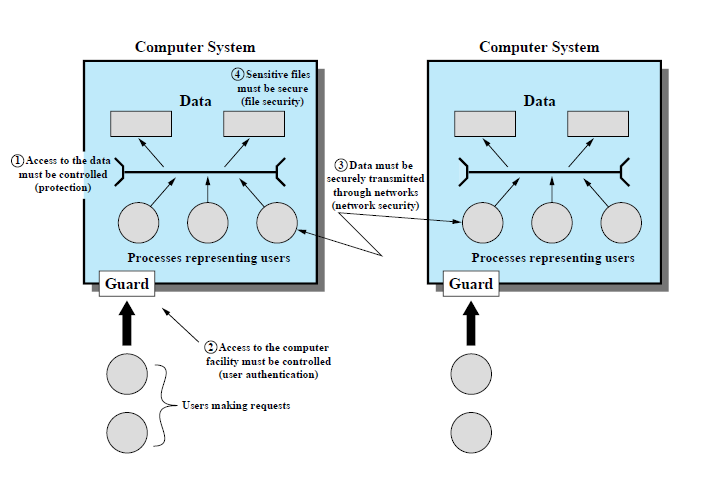
\includegraphics{../immagini/scope_computer_security.png}
                            \caption{Scope of computer security}\footnotemark
                        \end{center}
                    \end{figure}
                    \footnotetext{This figure depicts security concerns other than physical security, including controlling of access to computers systems, safeguarding of data transmitted over communications systems, and safeguarding of stored data}
            \newpage
            \subsubsection{Passive and Active attacks}
                    \paragraph{Passive attacks}
                    \begin{itemize}
                        \item Attempts to learn or make use of information from the system but does not affect system resources
                        \item Eavesdropping on, or monitoring of, transmissions
                        \item Goal of attacker is to obtain information that is being transmitted
                        \item Two types:
                        \begin{itemize}
                            \item Release of message contents
                            \item Traffic analysis
                        \end{itemize}
                    \end{itemize}
                    \paragraph{Active Attacks}
                        \begin{itemize}
                            \item Attempts to alter system resources or affect their operation
                            \item Involve some modification of the data stream or the creation of a false stream
                            \item Four categories:
                            \begin{itemize}
                                \item Replay
                                \item Masquerade
                                \item Modification of messages
                                \item Denial of service
                            \end{itemize}
                        \end{itemize}
            \subsubsection{Question \& Examples}
                    \subparagraph{Question} \textit{HOW WOULD YOU CLASSIFY THE FOLLOWING ATTACK?
                    UPON STEALING A BANK CUSTOMER'S COMMERCIAL IDENTITY (E.G., THEIR
                    CREDIT CARD OR ACCOUNT INFORMATION), THE ATTACKER PRESENTS
                    THOSE CREDENTIALS FOR THE MALICIOUS PURPOSE OF USING THE
                    CUSTOMER'S CREDIT LINE TO STEAL MONEY}
        \newpage
        \subsection{Functional requirements}
                \subsubsection{Classification of Contermeasures}
                Several classifications of countermeasures aimed at reducing vulnerabilities and dealing with threats. Classification according to functional requirements:      
                defined in FIPS 200 (Minimum Security Requirements for Federal Informationand Information Systems). 
                This standard enumerates 17 security-related areas: They encompass a wide range of countermeasures to security vulnerabilities and threats. Roughly, they can be divided into two categories: \textbf{technical measures} and \textbf{management issues}.
                \paragraph{Technical Measures}
                        \begin{description}
                            \item[Access Control] \textbf{Limit} information system access to authorized users and of processes that act on their behalf; \textbf{Limit} the types of transactions and functions that authorized users are permitted to exercise. 
                            \item[Identification and Authentication] \textbf{Identify} system users, processes acting on behalf of users, or devices; \textbf{Authenticate} (or verify) the identities of those users, processes, or devices, as a prerequisite to allowing access.
                            
                            \item[System and Communications Protection]: 
                            
                            \begin{itemize}
                                \item Monitor, control, and protect organizational communications (both transmitted and received) at the external boundaries and key internal boundaries of the information systems
                                \item Employ architectural designs, software development techniques, and systems engineering principles that promote effective information security within organizational information systems
                            \end{itemize}
                            \item [System and Information Integrity]:
                             
                            \begin{itemize}
                                \item Identify, report, and correct information and information system flaws in a timely manner
                                \item Provide protection from malicious code at appropriate locations within organizational information systems
                                \item Monitor information system security alerts and advisories and take appropriate actions in response
                            \end{itemize}
                            
                        \end{description}
                \paragraph{Management measures}
                        \begin{description}
                            \item[Systems and Services Acquisition]:
                            \begin{itemize}
                                \item Allocate sufficient resources to adequately protect organizational information systems
                                \item Employ system development life cycle processes that incorporate information security considerations
                                \item Employ software usage and installation restrictions
                                \item Ensure that third-party providers employ adequate security measures to protect information, applications, and/or services outsourced from the organization
                            \end{itemize}
                            \item[Awareness and Training]: 
                            \begin{itemize}
                                \item Address managers and users of organizational information systems
                                \item Make them aware of the security risks and of the applicable laws, regulations, and policies
                                \item Train all the personnel to carry out their duties according to the security protocols
                            \end{itemize}
                            \item[Audit and Accountability]:Create, protect, and retain information system audit records to enable the monitoring, analysis, investigation, and reporting of unlawful, unauthorized, or inappropriate information system activity. Ensure that the actions of individual users can be uniquely traced so they can be held accountable for their actions.
                            \item[Certification, Accreditation, and Security Assessments]:
                            \begin{itemize}
                                \item Periodically assess the security controls to determine their effectiveness
                                \item Develop and implement plans of action designed to correct deficiencies and reduce or eliminate vulnerabilities
                                \item Monitor information system security controls on an ongoing basis to ensure the continued effectiveness of the controls
                            \end{itemize}
                            \item[Contingency Planning]:  
                            \begin{itemize}
                                \item Establish, maintain, and implement plans for emergency response, backup operations, and post-disaster recovery
                                \item Ensure the availability of critical information resources and continuity of operations in emergency situations
                            \end{itemize}
                            \item[Maintenance]: 
                            \begin{itemize}
                                \item Perform periodic and timely maintenance on organizational information systems
                                \item Provide effective controls on the tools, techniques, mechanisms, and personnel used to conduct information system maintenance
                            \end{itemize}
                            \item [Physical and Environmental Protection]:
                            \begin{itemize}
                                \item Limit physical access to information systems, equipment, and the respective operating environments to authorized individuals
                                \item Protect the physical plant and support infrastructure for information systems
                                \item Provide supporting utilities for information systems
                                \item Protect information systems against environmental hazards
                                \item Provide appropriate environmental controls in facilities containing information systems
                            \end{itemize}
                            \item [Planning]:
                            \begin{itemize}
                                \item Develop, document, periodically update, and implement security plans
                                \item The security plans describe the security controls in place or planned for the information systems and the rules of behavior for individuals accessing the system
                            \end{itemize}
                            \item [Personnel Security]: 
                            \begin{itemize}
                                \item Ensure that individuals with positions of responsibility (including third-parties) are trustworthy and meet the security criteria for those positions
                                \item Ensure that organizational information and information systems are protected during and after personnel actions such as terminations and transfers
                                \item Employ formal sanctions for personnel failing to comply with organizational security policies and procedures
                            \end{itemize}
                            \item [Risk Assessment]:
                            \begin{itemize}
                                \item Periodically assess the risk to organizational operations (including mission, functions, image, or reputation), organizational assets, and individuals
                                \item Risks may result from the operation of organizational information systems and the associated processing, storage, or transmission of organizational information
                            \end{itemize}
                                                                            
                        \end{description}
            \paragraph{Overlap functional areas}
                        \begin{description}
                            \item[Configuration Management]: 
                            \begin{itemize}
                                \item Establish and maintain baseline configurations and inventories of organizational information systems (hardware, software, documents, etc.) throughout the respective system development life cycles
                                \item Establish and enforce security configuration settings for information technology products employed
                            \end{itemize}
                            \item [Incident Response]: 
                            \begin{itemize}
                                \item Establish an operational incident-handling capability (includes preparation, detection, analysis, containment, recovery, and user-response activities)
                                \item Track, document, and report incidents to appropriate organizational officials and/or authorities
                            \end{itemize}
                            \item [Media Protection]: 
                            \begin{itemize}
                                \item Protect information system media, both paper and digital
                                \item Limit access to information on information system media to authorized users
                                \item Sanitize or destroy information system media before disposal or release for reuse
                            \end{itemize}
                            
                        \end{description}
            \subsubsection{Fundamental Security Design Principles} 
            \begin{description}
                \item[Economy of Mechanism] Keep security measures simple and small to reduce vulnerabilities and maintenance efforts.
                \item[Fail-safe Default] Base access decisions on permission rather than exclusion to ensure a safer failure mode.
                \item[Complete Mediation] Check every access against the access control mechanism to prevent reliance on cached decisions.
                \item[Open Design] Design security mechanisms openly to allow for public scrutiny and confidence in their effectiveness.
                \item[Separation of Privilege] Use multiple privilege attributes to access restricted resources, mitigating potential damage from security attacks.
                \item[Least Privilege] Restrict processes and users to the minimum set of privileges required for their tasks to minimize risks.
                \item[Least Common Mechanism] Minimize shared functions between users to reduce unintended communication paths and security implications.
                \item[Psychological Acceptability] Ensure security mechanisms do not unduly interfere with user work and are transparent and intuitive.
                \item[Isolation] Isolate public access systems from critical resources and isolate processes and files of individual users to prevent unauthorized access.
                \item[Encapsulation] Protect data objects by encapsulating procedures and data objects within their own domain.
                \item[Modularity] Develop security functions as separate modules and use a modular architecture to support upgrades without redesigning the entire system.
                \item[Layering] Employ multiple, overlapping protection approaches to address people, technology, and operational aspects of information systems.
                \item[Least Astonishment] Ensure programs and user interfaces respond in a way that is least likely to astonish users, promoting intuitive understanding of security mechanisms.
            \end{description}
            \subsubsection{Question \& Examples}
                        \subparagraph{Question}: 
                        \begin{enumerate}
                            \item Encryption of the SSD of a laptop
                            \item Keeping the hash of executable files of the OS in a CD
                            \item Uninstallation from the system of unused applications
                        \end{enumerate}
                        \subparagraph{Answer}:
                            \begin{enumerate}
                                \item Media Protection
                                \item System and Information integrity
                                \item Configuration Management
                            \end{enumerate}
                        \subparagraph{Question}:\\
                        Consider the following general code for allowing access to a resource:
                            \begin{lstlisting}
                                DWORD dwRet= IsAccessAllowed(...);

                                
                                if (dwRet== ERROR_ACCESS_DENIED) {
                                    // Security check failed.
                                    // Inform user that access is denied.
                                } else {
                                    // Security check OK.
                                }
                            \end{lstlisting}
                            \begin{itemize}
                                \item Explain the security flaw in this program.
                                \item Rewrite the code to avoid the flaw.
                            \end{itemize}
                        \subparagraph{Answer}
                        Chiedere a lezione ...
        \subsection{Attack surfaces and security strategies}
             \subsubsection{Attack surfaces}
             Consist of the reachable and exploitable vulnerabilities in a system
             Examples:\\
             \begin{itemize}
                \item Open ports on outward facing Web and other servers, and code listening on those ports
                \item Services available on the inside of a firewall
                \item Code that processes incoming data, email, XML, office documents, and industry-specific custom data exchange formats
                \item Interfaces, SQL, and Web forms
                \item An employee with access to sensitive information vulnerable to a social engineering attack
            \end{itemize}
                \paragraph{Categories}
                    \subparagraph{Network Attack Surface}
                    \begin{itemize}
                        \item Vulnerabilities over an enterprise network, wide-area network, or the Internet
                        \item Network protocol vulnerabilities (e.g., those used for DoS attacks)
                        \item Disruption of communications links
                        \item Various forms of intruder attacks
                    \end{itemize}
                    
                    \subparagraph{Software Attack Surface}
                    \begin{itemize}
                        \item Vulnerabilities in application, utility, or operating system code
                        \item Particular focus on Web server software
                    \end{itemize}
                    
                    \subparagraph{Human Attack Surface}
                    \begin{itemize}
                        \item Vulnerabilities created by personnel or outsiders, such as social engineering, Human error, Trusted insiders
                    \end{itemize}
                \newpage
                \paragraph{Analysis}
                    \subparagraph{To assess the scale and severity of threats to a system:}
                    \begin{itemize}
                        \item Identifies the points of vulnerability
                        \item Identifies the most appropriate security mechanisms and their deployment
                      \end{itemize}
                    \subparagraph{Uses:}
                        \begin{itemize}
                            \item Makes developers and security analysts aware of where security mechanisms are required.
                            \item Designers may be able to find ways to make the surface smaller, thus making the task of the adversary more difficult.
                            \item It also provides guidance on setting priorities for testing, strengthening security measures, or modifying the service or application.
                        \end{itemize}
                    
                    \begin{figure}[h]
                        \begin{center}
                        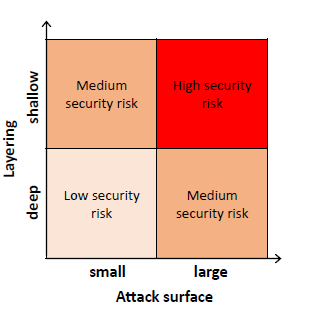
\includegraphics{../immagini/Defense_in_depth.png}
                        \end{center}
                    \end{figure}
                \paragraph{Trees}
               
                \subparagraph{An attack tree is a branching, hierarchical data structure that represents a set of potential techniques for exploiting security vulnerabilities:}
                \begin{itemize}
                    \item The root of the tree is the security incident (the goal of the attack).
                    \item The branches and subnodes of the tree are the ways that an attacker could reach that goal.
                    \item Each subnode defines a subgoal, and each subgoal may have its own set of further subgoals, etc.
                    \item The leaf nodes represent different ways to initiate an attack. 
                \end{itemize}

                \subparagraph{Each node other than a leaf is either an AND-node or an OR-node:}
                    \begin{itemize}
                        \item To achieve the goal represented by an AND-node, the subgoals represented by all of that node’s subnodes must be achieved.
                        \item For an OR-node, at least one of the subgoals must be achieved.
                    \end{itemize}

                \subparagraph{Branches can be labeled with values representing difficulty, cost, or other attack attributes, so that alternative attacks can be compared.}
                \subparagraph{Attack trees allow analysis of attack patterns:}
                    \begin{itemize}
                        \item To build a body of knowledge about both attack strategies and patterns.
                        \item To document security attacks in a structured form that reveals key vulnerabilities.
                        \item To guide the design of systems and applications, and the choice and strength of countermeasures.
                    \end{itemize}
                \begin{figure}
                    \begin{center}
                    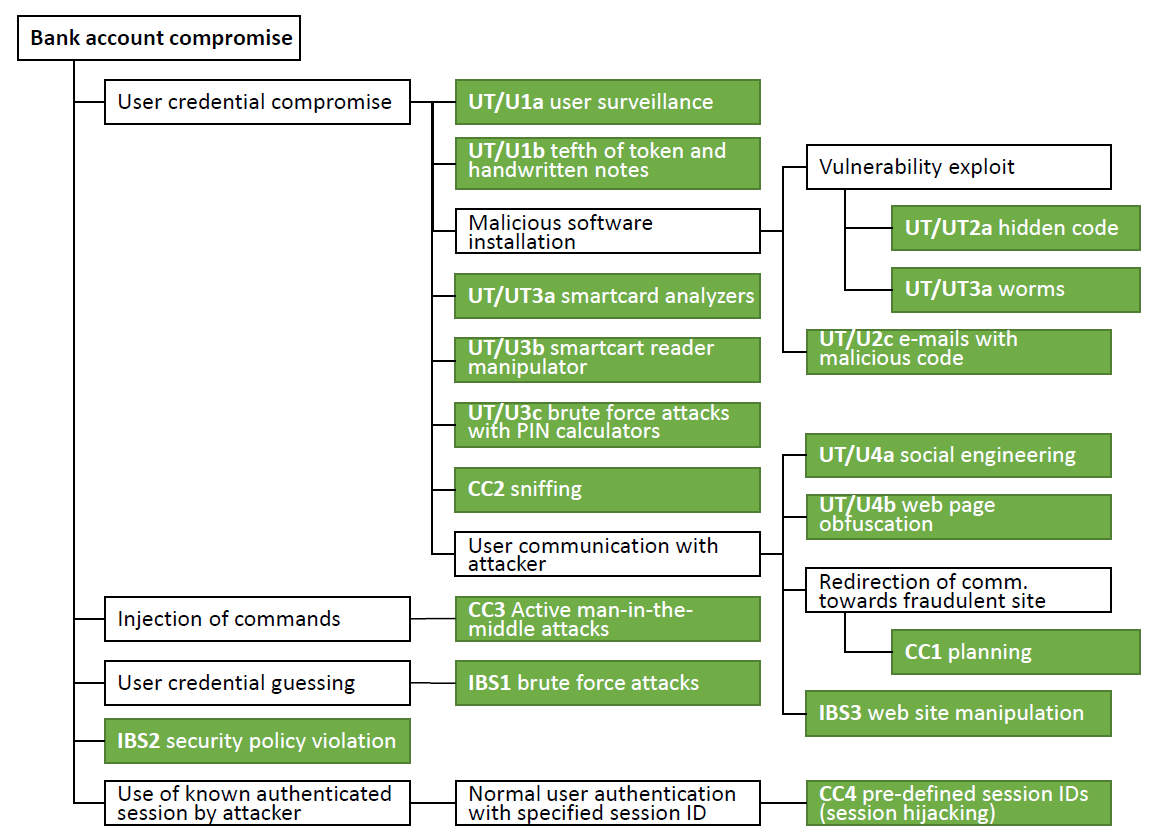
\includegraphics[scale=0.5]{../immagini/Example_attack_tree.png}
                    \caption{An attack tree for internet banking authentication}
                    \end{center}
                \end{figure}


                \paragraph{Question \& Examples}
                    \textbf{Q:} CAN YOU MAKE AN EXAMPLE OF SOMETHING THAT MAY ENLARGE THE
                    ATTACK SURFACE ON YOUR PC?
                    \textbf{A:}
                    Example of Enlarging the Attack Surface on Your PC
                    One example of something that may enlarge the attack surface on your PC is installing unnecessary software or applications. Each piece of software you install can introduce new vulnerabilities that attackers might exploit. Here is a detailed breakdown of how this can happen:

                            \subparagraph{Increased Number of Potential Vulnerabilities}
                            \begin{itemize}
                                \item Each installed application has its own codebase and, potentially, its own vulnerabilities. By adding more software, you increase the total number of vulnerabilities that might exist on your system.
                                \item \textbf{Example:} Installing a new media player that has a known buffer overflow vulnerability.
                            \end{itemize}

                            \subparagraph{Additional Network Services}
                            \begin{itemize}
                                \item Some software might install additional network services or open network ports, which could be exploited by attackers.
                                \item \textbf{Example:} A file-sharing application that opens new ports and can be accessed remotely.
                            \end{itemize}

                            \subparagraph{Expanded Attack Vectors}
                            \begin{itemize}
                                \item New software can introduce new attack vectors. For instance, a program that integrates with your browser might create opportunities for drive-by download attacks or malicious extensions.
                                \item \textbf{Example:} Installing a browser toolbar that inadvertently allows cross-site scripting (XSS) attacks.
                            \end{itemize}

                            \subparagraph{Third-Party Software Dependencies}
                            \begin{itemize}
                                \item Many applications rely on third-party libraries or components. These dependencies might not be updated as frequently and could contain vulnerabilities.
                                \item \textbf{Example:} An outdated version of a library used by a photo editing software.
                            \end{itemize}

                            \subparagraph{Increased Complexity}
                            \begin{itemize}
                                \item The more software you have, the more complex your system becomes. This increased complexity can make it harder to manage and secure your system effectively.
                                \item \textbf{Example:} Multiple security tools installed that may conflict with each other, reducing overall security effectiveness.
                            \end{itemize}
                    \newpage
                    \textbf{Q:}
                    DRAW AN ATTACK TREE FOR GAINING ACCESS TO THE CONTENT OF A
                    PHYSICAL SAFE\\
                    \textbf{A:}
                    
                
                      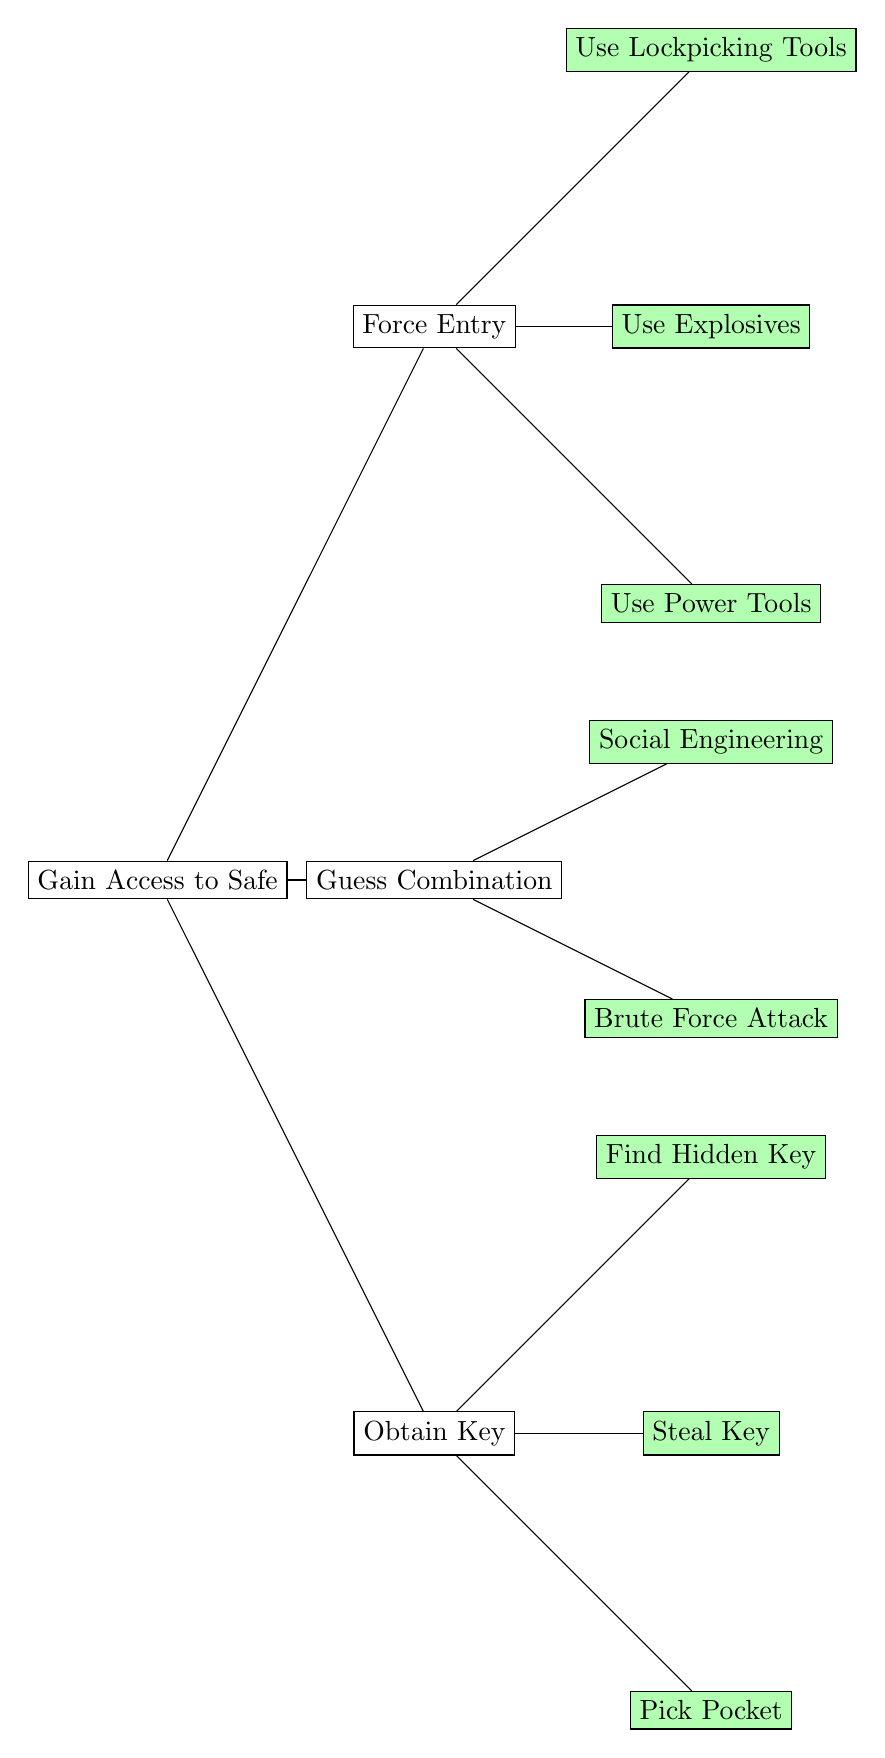
\begin{tikzpicture}[
                        edge from parent/.style={draw, -},
                        every node/.style={rectangle, draw, align=center},
                        grow=east,
                        sibling distance=12em,
                        level distance=10em,
                        level 1/.style={sibling distance=20em},
                        level 2/.style={sibling distance=10em}
                        ]
                      
                        \node {Gain Access to Safe}
                          child {node {Obtain Key}
                            child {node [fill=green!30] {Pick Pocket}}
                            child {node [fill=green!30] {Steal Key}}
                            child {node [fill=green!30] {Find Hidden Key}}
                          }
                          child {node {Guess Combination}
                            child {node [fill=green!30] {Brute Force Attack}}
                            child {node [fill=green!30] {Social Engineering}}
                          }
                          child {node {Force Entry}
                            child {node [fill=green!30] {Use Power Tools}}
                            child {node [fill=green!30] {Use Explosives}}
                            child {node [fill=green!30] {Use Lockpicking Tools}}
                          };
                      \end{tikzpicture}
            \newpage
            \subsubsection{Security strategies}
                      \paragraph{Security Policy}
                        \subparagraph{Several factors to be considered in the development of a security policy:}
                            \begin{itemize}
                                \item The value of the assets being protected
                                \item The vulnerabilities of the system
                                \item Potential threats and the likelihood of attacks
                            \end{itemize}
                        \subparagraph{Relevant tradeoffs:}
                          \begin{itemize}
                              \item Ease of use versus security
                              \item Cost of security versus cost of failure and recovery
                          \end{itemize}
                        \subparagraph{The security policy is a business decision, possibly influenced by legal requirements.}
                    \paragraph{Security implementation}
                    \begin{description}
                        \item[Prevention:] An ideal security scheme is one in which no attack is successful…
                        \begin{itemize}
                            \item Example: transmission of encrypted data
                        \end{itemize}
                        
                        \item[Detection:] Absolute protection is often not feasible, but it is practical to detect security attacks.
                        \begin{itemize}
                            \item Example: intrusion detection systems designed to detect the presence of unauthorized individuals logged onto a system.
                        \end{itemize}
                        
                        \item[Response:] If security mechanisms detect an ongoing attack, the system may be able to respond in such a way as to halt the attack and prevent further damage.
                        
                        \item[Recovery:] An example of recovery is the use of backup systems, so that if data integrity is compromised, a prior, correct copy of the data can be reloaded.
                    \end{description}
                            \paragraph{Assurance and Evaluation}
                            
                            \begin{description}
                                \item[Assurance] is an attribute of a system that provides confidence that the system operates such that the system’s security policy is enforced.
                                \begin{itemize}
                                    \item Encompasses both system design and implementation.
                                    \item Deals with the questions:
                                    \begin{itemize}
                                        \item “Does the security system design meet its requirements?”
                                        \item “Does the security system implementation meet its specifications?”
                                    \end{itemize}
                                    \item It is expressed as a degree of confidence, not in terms of a formal proof that a design or implementation is correct.
                                    \item Absolute proofs not possible at the state of the art.
                                \end{itemize}
                                
                                \item[Evaluation] is the process of examining a computer product or system with respect to certain criteria.
                                \begin{itemize}
                                    \item Involves testing, formal analytic, or mathematical techniques.
                                \end{itemize}
                            \end{description}
                        \subsection{Standards}

                        \begin{description}
                            \item[National Institute of Standards and Technology (NIST):] NIST is a U.S. federal agency that deals with measurement science, standards, and technology related to U.S. government use and to the promotion of U.S. private sector innovation.
                            
                            \item[Internet Society (ISOC):] ISOC is a professional membership society that provides leadership in addressing issues that confront the future of the Internet, and is the organization home for the groups responsible for Internet infrastructure standards.
                            
                            \item[International Telecommunication Union (ITU-T):] ITU is a United Nations agency in which governments and the private sector coordinate global telecom networks and services.
                            
                            \item[International Organization for Standardization (ISO):] ISO is a nongovernmental organization whose work results in international agreements that are published as International Standards.
                        \end{description}

                        \subsection{Questions \& Examples}
                        \subparagraph{Question}
                        CONSIDER AN INFORMATION SYSTEM OF A SMART CITY IN WHICH CITIZENS
                        PROVIDE AN ID NUMBER AND A E-DOCUMENT FOR ACCOUNT ACCESS
                        THROUGH AUTOMATIC MACHINES.
                        GIVE EXAMPLES OF CONFIDENTIALITY, INTEGRITY, AND AVAILABILITY
                        REQUIREMENTS ASSOCIATED WITH THE SYSTEM. IN EACH CASE, INDICATE
                        THE DEGREE OF THE IMPORTANCE OF THE REQUIREMENT.
                        \subparagraph{Answer}
                        \begin{itemize}
                            \item  \textbf{Confidentiality Requirements:}
                            \begin{itemize}
                                \item The ID number and e-document provided by citizens should be encrypted during transmission and storage to prevent unauthorized access.
                                \item Importance : High. Ensuring confidentiality is crucial to protect citizens' sensitive personal information from unauthorized disclosure or misuse.
                            \end{itemize}
                            \item   \textbf{Integrity Requirements:}
                            \begin{itemize}
                                \item The information system should have mechanisms to detect unauthorized modification or tampering with citizens' ID numbers or e-documents.
                                \item Importance: High. Maintaining the integrity of the data is essential to ensure that citizens can trust the accuracy and reliability of the information provided by the system.
                            \end{itemize}
                            \item  \textbf{Availability Requirements:}
                            \begin{itemize}
                                \item The automatic machines should be operational and accessible to citizens 24/7, with minimal downtime for maintenance or repairs.
                                \item Importance: High. The availability of the system is critical to ensure that citizens can access the services they need at any time, especially in emergency situations.
                            \end{itemize}    
                        \end{itemize}
                        \subparagraph{Question}
                        CONSIDER A LAW ENFORCEMENT ORGANIZATION MANAGING EXTREMELY
                        SENSITIVE INVESTIGATIVE INFORMATION.
                        ASSIGN A LOW, MODERATE, OR HIGH IMPACT LEVEL FOR THE LOSS OF
                        CONFIDENTIALITY, AVAILABILITY, AND INTEGRITY, RESPECTIVELY.
                        JUSTIFY YOUR ANSWER.
                        \subparagraph{Answer}
                        \begin{description}
                            \item[Confidentiality Impact:]
                        \begin{itemize}
                            \item Loss of confidentiality: High
                            \begin{itemize}
                                \item Justification: The loss of confidentiality of sensitive investigative information could compromise ongoing investigations, reveal the identities of informants or undercover agents, and jeopardize national security or public safety.
                            \end{itemize}
                        \end{itemize}

                        \item[Availability Impact:]
                        \begin{itemize}
                            \item Loss of availability: Moderate
                            \begin{itemize}
                                \item Justification: While the loss of availability could disrupt access to critical information during investigations or operations, law enforcement organizations often have backup systems and procedures in place to mitigate the impact of temporary downtime.
                            \end{itemize}
                        \end{itemize}

                        \item[Integrity Impact:]
                        \begin{itemize}
                            \item Loss of integrity: High
                            \begin{itemize}
                                \item Justification: The loss of integrity could result in the manipulation or alteration of investigative data, leading to false evidence, wrongful convictions, or the compromise of the integrity of legal proceedings, undermining the trust in the justice system.
                            \end{itemize}
                        \end{itemize}

                    \end{description}
        \newpage
\section{Cryptogrphic tools}
                    \subsection{Symmetric Encryption}
                    The universal technique for providing confidentiality for
                    transmitted or stored data also referred to as conventional encryption or single-key
                    encryption. Two requirements for secure use: 
                    \begin{itemize}
                        \item Need a strong encryption algorithm
                        \item  Sender and receiver must have obtained copies of the
                        secret key in a secure fashion and must keep the key
                        secure
                    \end{itemize}

                    \begin{figure}[h]
                        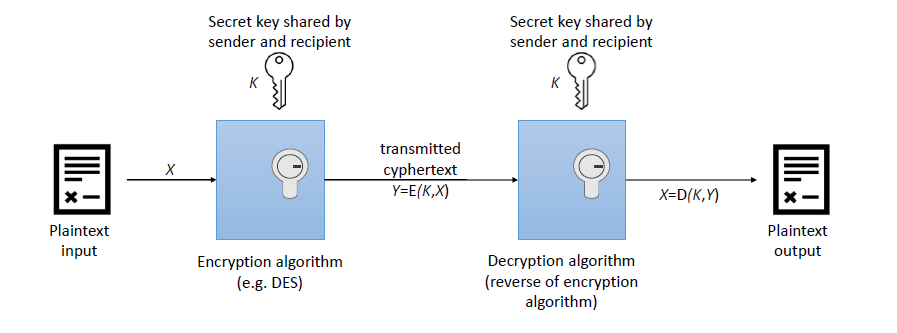
\includegraphics{../immagini/model_symmetric_security.png}
                        \caption{Simplified model of symmetric Encryption}
                    \end{figure}
                    
                        \subsubsection{Attacking symmetric encryption}
                            \paragraph{Cryptoanalytic attacks}
                            \begin{itemize}
                                \item Rely on:
                                \begin{itemize}
                                    \item Nature of the algorithm
                                    \item Some knowledge of the general characteristics of the plaintext
                                    \item Some sample plaintext-ciphertext pairs
                                \end{itemize}
                            \item Exploits the characteristics of the algorithm to attempt to deduce a specific plaintext or the key being used
                                \begin{itemize}
                                      
                                    \item If successful, all future and past messages encrypted with that key are compromised
                                \end{itemize}
                            \end{itemize}
                            \paragraph{Brute force attacks}
                            \begin{itemize}
                            \item Try all possible keys on some ciphertext until an intelligible translation into plaintext is obtained
                            \begin{itemize}
                                \item On average half of all possible keys must be tried to achieve success
                            \end{itemize}

                            
                        \end{itemize}
                  
                        
                                 \newpage   
                     
                        \subsubsection{Algorithm}
                                \begin{table}[h]
                                    \begin{center}
                                    \begin{tabular}{llll}
                                            \rowcolor[HTML]{34CDF9} 
                                                                        & DES & Triple DES & AES             \\
                                            Plaintext block size (bits)  & 64  & 64         & 128             \\
                                            \rowcolor[HTML]{96FFFB} 
                                            Ciphertext block size (bits) & 64  & 64         & 128             \\
                                            Key size (bits)              & 56  & 112 or 168 & 128,192, or 256
                                    \end{tabular}
                                \end{center}
                                    \caption{Comparison of Three Popular Symmetric Encryption Algorithms}
                                \end{table}
                            \paragraph{DES: Data Encryption Standard}
                                        \begin{itemize}
                                            \item Until recently was the most widely used encryption scheme
                                            \begin{itemize}
                                                \item FIPS PUB 46 (January 1977)
                                                \item Referred to as the Data Encryption Algorithm (DEA)
                                                \item Uses 64 bit plaintext block and 56 bit key to produce a 64 bit ciphertext block
                                            \end{itemize}
                                            \item Strength concerns:
                                            \begin{itemize}
                                                \item Concerns about the algorithm itself
                                                \begin{itemize}
                                                    \item DES is the most studied encryption algorithm in existence
                                                \end{itemize}
                                                \item Concerns about the use of a 56-bit key
                                                \begin{itemize}
                                                    \item The speed of commercial off-the-shelf processors makes this key length woefully inadequate
                                                \end{itemize}
                                            \end{itemize}
                                        \end{itemize}
                            \paragraph{Triple DES: 3DES}
                                        \begin{itemize}
                                            \item Repeats basic DES algorithm three times using either two or three unique keys
                                            \item First standardized for use in financial applications in ANSI standard X9.17 in 1985
                                            \item Attractions:
                                            \begin{itemize}
                                                \item 168-bit key length overcomes the vulnerability to brute-force attack of DES
                                                \item Underlying encryption algorithm is the same as in DES
                                            \end{itemize}
                                            \item Drawbacks:
                                            \begin{itemize}
                                                \item Algorithm is sluggish in software
                                                \item Uses a 64-bit block size
                                            \end{itemize}
                                        \end{itemize}
                            \paragraph{AES: Advanced Encryption Standard}
                                        \begin{itemize}
                                            \item Needed a replacement for 3DES
                                            \begin{itemize}
                                                \item Should have a security strength equal to or better than 3DES
                                                \item Significantly improved efficiency
                                                \item Symmetric block cipher
                                                \item 128-bit data and 128/192/256-bit keys
                                            \end{itemize}
                                            \item NIST called for proposals for a new AES in 1997
                                            \begin{itemize}
                                                \item Published as FIPS 197
                                                \item Selected Rijndael in November
                                            \end{itemize}
                                        \end{itemize}
                            \paragraph{Pratical Security Issues}
                            \begin{itemize}
                                \item Typically symmetric encryption is applied to a unit of data larger than a single 64-bit or 128-bit block
                                \item Electronic codebook (ECB) mode is the simplest approach to multiple-block encryption
                                \begin{itemize}
                                    \item Each block of plaintext is encrypted using the same key
                                    \item Cryptanalysts may be able to exploit regularities in the plaintext
                                \end{itemize}
                                \item Modes of operation
                                \begin{itemize}
                                    \item Alternative techniques developed to increase the security of symmetric block encryption for large sequences
                                    \item Overcomes the weaknesses of ECB
                                \end{itemize}
                            \end{itemize}        
                        \subsubsection{Types of symmetric encryption}
                            
                            \begin{figure}[h]
                                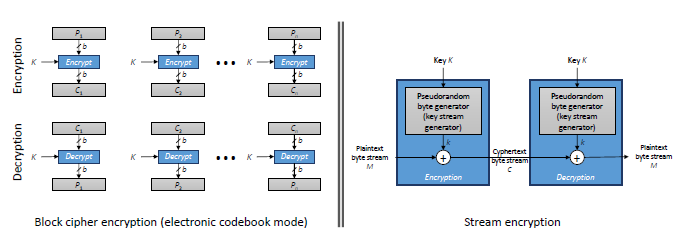
\includegraphics{../immagini/Types_of_symmetric_encryption.png}
                            \end{figure}
                            \paragraph{Block cyphers}
                                    \begin{itemize}
                                        \item With the Electronic Codebook (ECB) mode:
                                        \begin{itemize}
                                            \item A plaintext of length nb is divided into n b-bit blocks (P1, P2, ..., Pn).
                                            \item Each block is encrypted using the same algorithm and the same encryption key, to produce a sequence of n b-bit blocks of ciphertext (C1, C2, ..., Cn).
                                        \end{itemize}
                                        \item Security concerns:
                                        \begin{itemize}
                                            \item A cryptanalyst may exploit regularities in the plaintext to ease the task of decryption.
                                            \item For example, if it is known that the message always starts out with certain predefined fields, then the cryptanalyst may have a number of known plaintext-ciphertext pairs to work with.
                                        \end{itemize}
                                    \end{itemize}
                            \paragraph{Stream cyphers}
                            \begin{itemize}
                                \item The key is input to a pseudorandom bit generator that produces a stream of numbers that are apparently random.
                                \begin{itemize}
                                    \item A pseudorandom stream is unpredictable without knowledge of the input key.
                                \end{itemize}    
                                \item The output of the generator, called a keystream, is combined one byte at a time with the plaintext stream using the bitwise exclusive-OR (XOR) operation.
                                \item A stream cipher can also operate on one bit at a time or on units larger than a byte at a time.
                                \item A stream cipher can be as secure as a block cipher of comparable key length.
                                \begin{itemize}
                                    \item With a properly designed pseudorandom number generator.
                                \end{itemize}
                                \item Stream ciphers are typically faster and use far less code than block ciphers.
                                \item However, with a block cipher the keys can be reused.
                                \item Stream ciphers are good for encryption/decryption of data streams.
                                \begin{itemize}
                                    \item Data communications channel or a browser/Web link.
                                \end{itemize}
                                \item Block ciphers are good for file encryption, e-mail, databases etc.
                                \item However, both can be used in virtually any application.
                            \end{itemize}

                            \begin{table}[h]
                                \begin{center}

                            \begin{tabular}{|p{6cm}|p{6cm}|}
                                \hline
                                \textbf{Block Cipher} & \textbf{Stream Cipher} \\
                                \hline
                                \begin{itemize}
                                  \item Processes the input one block of elements at a time
                                  \item Produces an output block for each input block
                                  \item Can reuse keys
                                  \item More common
                                \end{itemize}
                                &
                                \begin{itemize}
                                  \item Processes the input elements continuously
                                  \item Produces output one element at a time
                                  \item Primary advantage is that they are almost always faster and use far less code
                                  \item Encrypts plaintext one byte at a time
                                  \item Pseudorandom stream is one that is unpredictable without knowledge of the input key
                                \end{itemize} \\
                                \hline
                              
                                \end{tabular}
                            \end{center}
                                \caption{Difference}
                            \end{table}
                        
                        \subsubsection{Questions \& Examples}
                            \subparagraph{Question}
                            HOW IS CRYPTANALYSIS
                            DIFFERENT FROM BRUTEFORCE
                            ATTACK?
                            \subparagraph{Answer} 
                           
                       


                            \begin{itemize}
                                \item \textbf{Approach}:
                                \begin{itemize}
                                    \item \textbf{Cryptanalysis}: Involves understanding and exploiting weaknesses in the encryption algorithm or its implementation.
                                    \item \textbf{Brute-Force Attacks}: Involve trying every possible key to decrypt the ciphertext.
                                \end{itemize}

                                \item \textbf{Knowledge Requirement}:
                                \begin{itemize}
                                    \item \textbf{Cryptanalysis}: Often requires specialized knowledge of mathematics, statistics, or the specific encryption algorithm.
                                    \item \textbf{Brute-Force Attacks}: Do not require specific knowledge beyond the ability to generate keys and test them.
                                \end{itemize}

                                \item \textbf{Speed}:
                                \begin{itemize}
                                    \item \textbf{Cryptanalysis}: Can potentially be faster than brute-force attacks if effective vulnerabilities are identified, especially for large key sizes where brute-force becomes impractical.
                                \end{itemize}
                            \end{itemize}

                            \subparagraph{Question}
                            WHAT ARE THE (TWO) PRINCIPAL
                            REQUIREMENTS FOR THE SECURE
                            USE OF SYMMETRIC ENCRYPTION?
                            \subparagraph{Answer}
                            \begin{enumerate}
                                \item \textbf{Key Management}:
                                \begin{itemize}
                                    \item Secure generation of keys: Keys should be generated using a secure random number generator.
                                    \item Distribution of keys: Keys must be securely distributed to authorized parties without interception by unauthorized entities.
                                    \item Key storage: Keys should be stored securely to prevent unauthorized access.
                                    \item Key update and rotation: Regular updates of keys and periodic rotation are essential to mitigate the risk of compromise.
                                \end{itemize}
                                
                                \item \textbf{Algorithm Selection and Implementation}:
                                \begin{itemize}
                                    \item Choosing strong algorithms: Use of well-established and cryptographically strong algorithms (e.g., AES-256) that are resistant to known attacks.
                                    \item Secure implementation: Implementation of the encryption algorithm must follow best practices and standards to avoid vulnerabilities such as side-channel attacks or implementation flaws.
                                    \item Regular security audits: Periodic security audits and evaluations of the encryption implementation to ensure it meets current security standards and practices.
                                \end{itemize}
                            \end{enumerate}
                    \subsection{Message authentication and hash functions}
                            \subsubsection{Message authentication}
                                \paragraph{Message authentication without confidentiality:}
                                        Message encryption by itself does not provide a secure form of authentication. It is possible to combine authentication and confidentiality in a single algorithm by encrypting a message along with its authentication tag. Typically, message authentication is provided as a separate function from message encryption.
                                        Situations in which message authentication without confidentiality
                                        may be preferable include:
                                        \begin{enumerate}
                                            \item There are a number of applications in which the same message is broadcast to a number of destinations.
                                            \item An exchange in which one side has a heavy load and cannot afford the time to decrypt all incoming messages.
                                            \item Authentication of a computer program in plaintext is an attractive service.
                                        \end{enumerate}
                                        Thus, there is a place for both authentication and encryption in
                                        meeting security requirements
                                \paragraph{MAC: Message Authentication Code}
                                A small block of data (the message authentication code –
                                MAC) is appended to the message to be authenticated
                                 MAC generated by means of a secret key: 
                                    \[
                                    \text{MAC} = \text{Func}(\text{Key}, \text{Message})
                                    \]
                                    The secret key is shared between the two communicating
                                    parties

                                    \begin{figure}[h]
                                        \begin{center}
                                            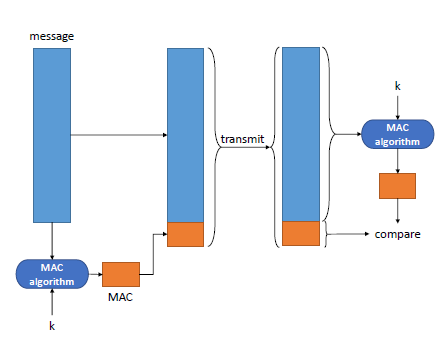
\includegraphics{../immagini/MAC.png}
                                        \end{center}
                                        \caption{Message
                                        authentication
                                        using a MAC}
                                    \end{figure}
                                    \subparagraph{Properties}
                                    \begin{enumerate}
                                        \item \textbf{Message Integrity}
                                        \begin{itemize}
                                            \item The receiver is assured that the message has not been altered.
                                            \item If an attacker alters the message but does not alter the code, then the receiver’s calculation of the code will differ from the received code.
                                            \item Because the attacker is assumed not to know the secret key, the attacker cannot alter the code to correspond to the alterations in the message.
                                        \end{itemize}
                                        \item \textbf{Message Authentication}
                                        \begin{itemize}
                                            \item The receiver is assured that the message is from the alleged sender.
                                            \item Because no one else knows the secret key, no one else could prepare a message with a proper code.
                                        \end{itemize}
                                        \item \textbf{Proper Sequence Assurance}
                                        \begin{itemize}
                                            \item The receiver is assured of the proper sequence if the message includes a sequence number.
                                            \item As in X.25, HDLC, and TCP.
                                            \item The attacker cannot successfully alter the sequence number.
                                        \end{itemize}
                                    \end{enumerate}
                            \subsubsection{One-way hash functions}
                                    \paragraph{Propreties}
                                    \begin{enumerate}
                                        \item It can be applied to data blocks of any size.
                                        \item It produces a fixed length output.
                                        \item It is easy to compute (making both software or hardware implementations practical).
                                        \item It is one way: it is computationally infeasible to find \( x \) such that \( H(x) = h \).
                                        \item It is weak collision resistant: given \( x \) it is computationally infeasible to find \( y \) such that \( H(x) = H(y) \).
                                        \item It is collision resistant: it is computationally infeasible to find a pair \( x, y \) such that \( H(x) = H(y) \).
                                    \end{enumerate}
                                    \begin{figure}
                                        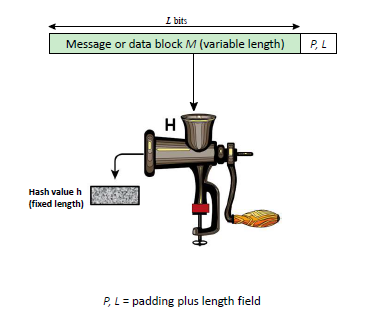
\includegraphics{../immagini/hash function.png}
                                    \end{figure}
                                    \paragraph{Message authentication with one-way hash functions}
                                    The hash function takes a variable-size message \( M \) and produces a fixed-size message digest \( H(M) \). Typically, the message is padded out to an integer multiple of some fixed length (e.g., 1024 bits). The padding includes the value of the length of the original message in bits. The length field is a security measure to increase the difficulty for an attacker to produce an alternative message with the same hash value. Unlike encryption algorithms, the hash function does not need a secret key.
                            \subsubsection{Alternative way of authenticating a message}
                                \begin{figure}[h]
                                    \begin{center}
                                    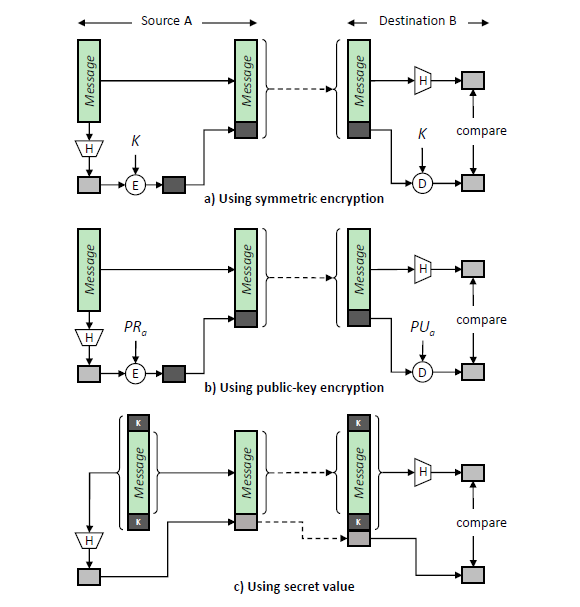
\includegraphics[scale=0.6]{../immagini/alternative.png}
                                    \end{center}
                                    \caption{Alternative way}
                                \end{figure}
                                \begin{enumerate}[label=\alph*]
                                    \item The message digest is encrypted using symmetric encryption.
                                    \begin{itemize}
                                        \item Only the sender and receiver know the encryption key.
                                        \item Assures the authenticity of the digest.
                                    \end{itemize}
                                    \item The message digest is encrypted using public-key encryption.
                                    \begin{itemize}
                                        \item Provides a digital signature as well as message authentication.
                                        \item Does not require the distribution of keys to communicating parties.
                                    \end{itemize}
                                    \item The method avoids encryption!
                                    \begin{itemize}
                                        \item \textbf{Advantages:}
                                        \begin{itemize}
                                            \item Software encryption is rather slow (even if the message is short, there may be several messages).
                                            \item Hardware encryption has costs and it is optimized for large data sizes.
                                            \item The encryption algorithm may be patented (and thus subject to royalties).
                                        \end{itemize}
                                        \item \textbf{Method based on the keyed hash MAC technique:}
                                        \begin{itemize}
                                            \item Assumes that two communicating parties, say A and B, share a common secret key \( K \).
                                            \item As long as \( K \) is secret, there’s no way for the attacker to modify the message or to generate a false message.
                                            \item Using \( K \) at the beginning and at the end makes the scheme more secure.
                                        \end{itemize}
                                    \end{itemize}
                                \end{enumerate}
                            \newpage
                            \subsubsection{Hash function for message authentication}
                                \paragraph{Proprieties}
                                \begin{itemize}
                                    \item Can be applied to a block of data of any size.
                                    \item Produces a fixed-length output.
                                    \item \( H(x) \) is relatively easy to compute for any given \( x \).
                                    \item One-way or pre-image resistant(In case (c), if this was not true it would be
                                    possible to find the secret key k! ):
                                    \begin{itemize}
                                        \item Given \( h \), it is computationally infeasible to find \( x \) such that \( H(x) = h \).
                                    \end{itemize}
                                    \item Given \( x \), it is computationally infeasible to find \( y \neq x \) such that \( H(y) = H(x) \).
                                          (Necessary to prevent forgery in cases (a), (b)
                                          and (c))
                                    \item Collision resistant or strong collision resistance:
                                         Computationally infeasible to find any pair \( (x,y) \) such that \( H(x) = H(y) \).
                                        \begin{itemize}
                                            \item Protects against an attack in which one party generates a message for another party to sign.
                                            \item For example:
                                            \begin{itemize}
                                                \item Suppose Bob gets to write an "I Owe You" message, sends it to Alice, and she signs it.
                                                \item Bob forges two messages with the same hash:
                                                \begin{itemize}
                                                    \item One message requires Alice to pay a small amount.
                                                    \item Another message requires Alice to pay a large amount.
                                                \end{itemize}
                                                \item Alice signs the first message, and Bob is then able to claim that the second message is authentic.
                                            \end{itemize}
                                        \end{itemize}
                                    
                                \end{itemize}
                                \begin{figure}[h]
                                    \begin{center}
                                        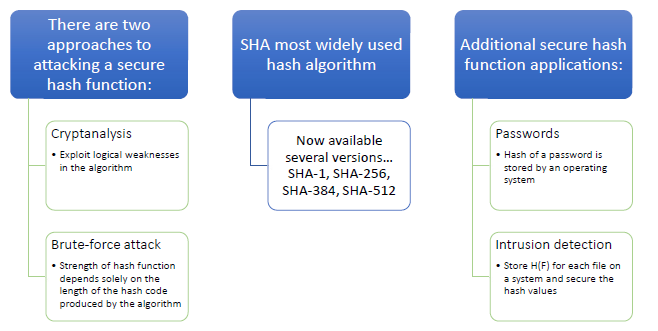
\includegraphics{../immagini/security_hash.png}
                                    \end{center}
                                    \caption{Security of hash functions}
                                \end{figure}

                                \subparagraph{Further
                                applications of
                                secure hash
                                functions}
                                \begin{itemize}
                                    \item \textbf{Passwords:}
                                    \begin{itemize}
                                        \item Some Operating Systems store hashes rather than passwords.
                                        \item When a user enters a password, the hash of that password is compared to the stored hash value for verification.
                                        \item The actual password is not retrievable even when accessing the password file.
                                    \end{itemize}
                                    \item \textbf{Intrusion detection:}
                                    \begin{itemize}
                                        \item Store \( H(F) \) for each file on a system and keep the hash values secure (e.g., on a CD-R that is kept secure).
                                        \item One can later determine if a file has been modified by recomputing \( H(F) \).
                                        \item An intruder would need to change \( F \) without changing \( H(F) \), which is not computationally feasible.
                                    \end{itemize}
                                \end{itemize}
                        \subsubsection{Question \& Examples}
                        \subparagraph{Question} WHICH ONE OF THE PREVIOUS
                        SCHEMAS GUARANTEES THE NONREPUDIATION
                        PROPERTY? (About Figure 6 )
                        \subparagraph{Answer}
                        The schema that guarantees the non-repudiation property is:

                        \begin{enumerate}
                            \item The message digest is encrypted using public-key encryption.
                            \begin{itemize}
                                \item Provides a digital signature as well as message authentication.
                                \item Does not require the distribution of keys to communicating parties.
                            \end{itemize}
                        \end{enumerate}
                        
                        This method provides a digital signature, which is crucial for non-repudiation. It ensures that the sender cannot deny having sent the message because the public-key encryption provides a verifiable proof of the sender's identity.
                        \subparagraph{Question}
                        WHY DOES THE HASH FUNCTION  NEED TO BE ONE-WAY?
                        \subparagraph{Answer}
                        The hash function needs to be one-way primarily for security reasons. This property ensures that given the output (hash value), it is computationally infeasible to determine the original input (message or data) that produced that hash.
                \subsection{Public-key encryption}
                            \subsubsection{Public-key encryption scheme}
                                \paragraph{Public key}
                                    \begin{figure}
                                        \begin{center}
                                            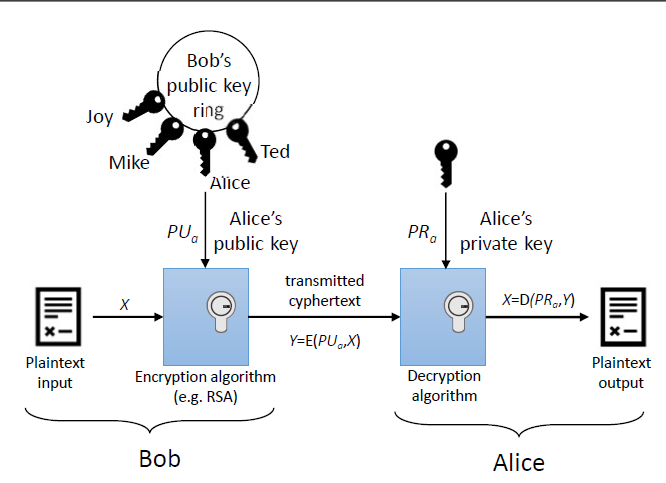
\includegraphics{../immagini/public_key.png}
                                        \end{center}
                                    \end{figure}
                                    \begin{description}
                                        \item[Plaintext] Readable message or data that is fed into the algorithm as input
                                        \item[Encryption algorithm] Performs transformations on the plaintext
                                        \item[Public and private key] Pair of keys, one for encryption, one for decryption
                                        \item[Ciphertext] Scrambled message produced as output
                                        \item[Decryption key] Produces the original plaintext
                                    \end{description}
                                \paragraph{Private key}
                                    \begin{figure}
                                        \begin{center}
                                            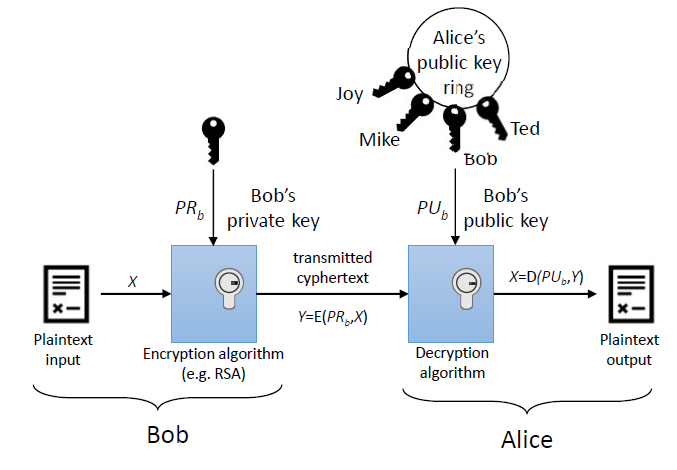
\includegraphics{../immagini/private_key.png}
                                        \end{center}
                                    \end{figure}
                                    \begin{itemize}
                                        \item User encrypts data using his or her own private key
                                        \item Anyone who knows the corresponding public key will be able to decrypt the message
                                    \end{itemize}
                            \subsubsection{Public-key Cryptosystems}
                                    \paragraph{Requirements}
                                    \begin{itemize}
                                        \item Computationally easy to create key pairs
                                        \item Useful if either key can be used for Requirements each role
                                        \item Computationally easy for sender knowing public key to encrypt messages
                                        \item Computationally infeasible for opponent to determine private key from public key
                                        \item Computationally easy for receiver knowing private key to decrypt ciphertext
                                        \item Computationally infeasible for opponent to otherwise recover original message
                                    \end{itemize}
                                    \newpage
                                    \paragraph{Algorithms}
                                    \begin{itemize}
                                        \item RSA (Rivest, Shamir, Adleman)
                                        \begin{itemize}
                                            \item Developed in 1977
                                            \item Most widely accepted and implemented approach to public-key encryption
                                            \item Block cipher in which the plaintext and ciphertext are integers between 0 and \(n-1\) for some \(n\)
                                        \end{itemize}
                                        \item Diffie-Hellman key exchange algorithm
                                        \begin{itemize}
                                            \item Enables two users to securely reach agreement about a shared secret that can be used as a secret key for subsequent symmetric encryption of messages
                                            \item Limited to the exchange of the keys
                                        \end{itemize}
                                        \item Digital Signature Standard (DSS)
                                        \begin{itemize}
                                            \item Provides only a digital signature function with SHA-1
                                            \item Cannot be used for encryption or key exchange
                                        \end{itemize}
                                        \item Elliptic curve cryptography (ECC)
                                        \begin{itemize}
                                            \item Security like RSA, but with much smaller keys
                                        \end{itemize}
                                    \end{itemize}

                                    \begin{table}[h]
                                        \begin{center}
                                            \begin{tabular}{| m{3cm} | m{3cm} | m{3cm} | m{3cm} |}
                                                \hline
                                                \textbf{Algorithm} & \textbf{Digital signature} & \textbf{Symmetric key distribution} & \textbf{Encryption of secret keys} \\
                                                \hline
                                                RSA & Yes & Yes & Yes \\
                                                \hline
                                                Diffie-Hellman & No & Yes & No \\
                                                \hline
                                                DSS & Yes & No & No \\
                                                \hline
                                                Elliptic Curve & Yes & Yes & Yes \\
                                                \hline
                                                \end{tabular}
                                        \end{center}
                                    \end{table}

                            \subsubsection{Digital Signatures}
                            NIST FIPS PUB 186-4 defines a digital signature as:
                                ”\textit{The result of a cryptographic transformation of data that,
                                when properly implemented, provides a mechanism for
                                verifying origin authentication, data integrity and signatory
                                non-repudiation.}” Thus, a digital signature is a data-dependent bit pattern, generated
                                by an agent as a function of a file, message, or other form of data
                                block FIPS 186-4 specifies the use of one of three digital signature
                                algorithms: 
                                \begin{description}
                                    \item[DSA] Digital Signature Algorithm  
                                    \item[RSA ] Digital Signature Algorithm
                                    \item[ ECDSA]Elliptic Curve Digital Signature Algorithm
                                \end{description}
                                \newpage
                                \begin{figure}
                                    \begin{center}
                                        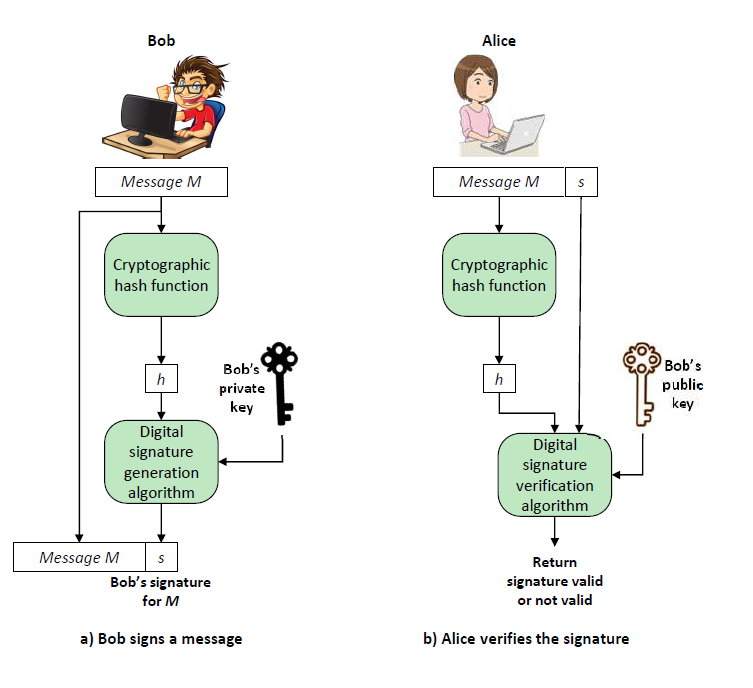
\includegraphics[scale=0.5]{../immagini/signature_process.png}
                                    \end{center}
                                    \caption{Essential
                                    elements of a
                                    digital signature
                                    process}
                                \end{figure}
                                \begin{figure}
                                    \begin{center}
                                        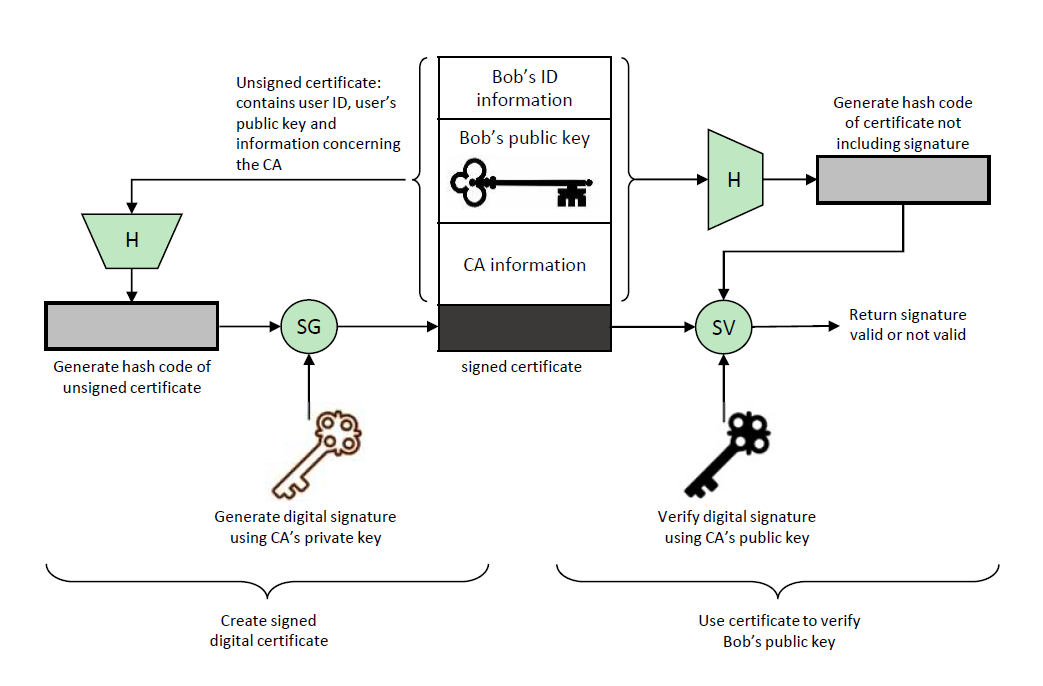
\includegraphics[scale=0.5]{../immagini/CA.png}
                                    \end{center}
                                    \caption{CA}\footnotemark
                                \end{figure}
                                \footnotetext{CA: certificate authority that is trusted by the user community
                           
                             government agency, financial institution, …}
                            \newpage
                             \paragraph{Digital envelopes}
                            A way to encrypt a message without
                            needing to first arrange for sender and
                            receiver to have the same secret key
                            \begin{figure}[h]
                                \begin{center}
                                    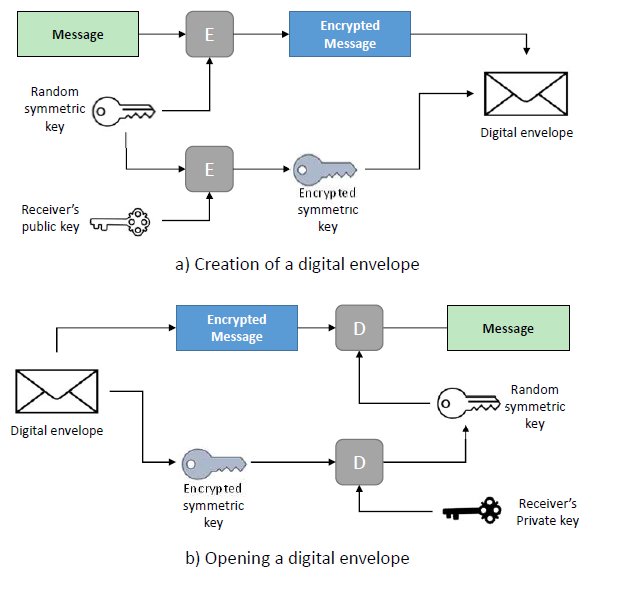
\includegraphics[scale=0.8]{../immagini/digital_envelope.png}
                                \end{center}
                                \caption{}
                            \end{figure}
        \newpage
        \subsection{Random numbers}
                            \subsubsection{Uses of
                            random
                            numbers uses}
                            \begin{itemize}
                                \item Keys for public-key algorithms
                                \item Stream key for symmetric stream cipher
                                \item Symmetric key for use as a temporary session key or in creating a digital envelope
                                \item Handshaking to prevent replay attacks
                                \item Session key
                            \end{itemize}

                            \subsubsection{Random number requirements}
                            \begin{itemize}
                                \item Randomness
                                \begin{itemize}
                                    \item Criteria:
                                    \begin{itemize}
                                        \item Uniform distribution
                                        \begin{itemize}
                                            \item Frequency of occurrence of each of the numbers should be approximately the same
                                        \end{itemize}
                        
                                        
                                        \item Independence
                                        \begin{itemize}
                                            \item No one value in the sequence can be inferred from the others
                                        \end{itemize}
                                    \end{itemize}
                                \end{itemize}
                                \item Unpredictability
                                        \begin{itemize}
                                            \item Each number is statistically independent of other numbers in the sequence
                                            \item Opponent should not be able to predict future elements of the sequence on the basis of earlier elements
                                        \end{itemize}
                                    \end{itemize}
                            \subsubsection{Random Vs Pseudorandom}
                            \begin{itemize}
                                \item Cryptographic applications typically make use of algorithms for random number generation
                                \begin{itemize}
                                    \item Algorithms are deterministic
                                    \item Produce sequences of numbers that are not statistically random
                                \end{itemize}
                                \item Pseudorandom numbers are:
                                \begin{itemize}
                                    \item Sequences produced that satisfy statistical randomness tests
                                    \item Likely to be predictable
                                \end{itemize}
                                \item True random number generator (TRNG):
                                \begin{itemize}
                                    \item Uses a nondeterministic source to produce randomness
                                    \item Most operate by measuring unpredictable natural processes (radiation, gas discharge, leaky capacitors)
                                    \item Increasingly provided on modern processors
                                \end{itemize}
                            \end{itemize}
                        \subsection{Question \& Examples}
                        \subparagraph{Questions}
                        The schema in figure 8 : 
                        \begin{enumerate}
                            \item provides confidentiality?
                            \item is Alice sure the message is from Bob?
                            \item is Alice sure the message has not been altered?
                        \end{enumerate}
                        \subparagraph{Answers} Da vedere
                        \subparagraph{Problem} THE SCHEMA (DIGITAL
                        ENVELOPE) IN FIGURE 10 DOES NOT GUARANTEE
                        THE AUTHENTICATION OF THE
                        SENDER.
                        CAN YOU IMPROVE THE SCHEMA
                        TO INCLUDE AUTHENTICATION?
                    \subsection{Exercise}
                                \subsubsection{Exercise 1}
                                    \subparagraph{Question}
                                    Draw an attack tree for gaining access to a (physical) office.
                                    \subparagraph{Answer}
                                    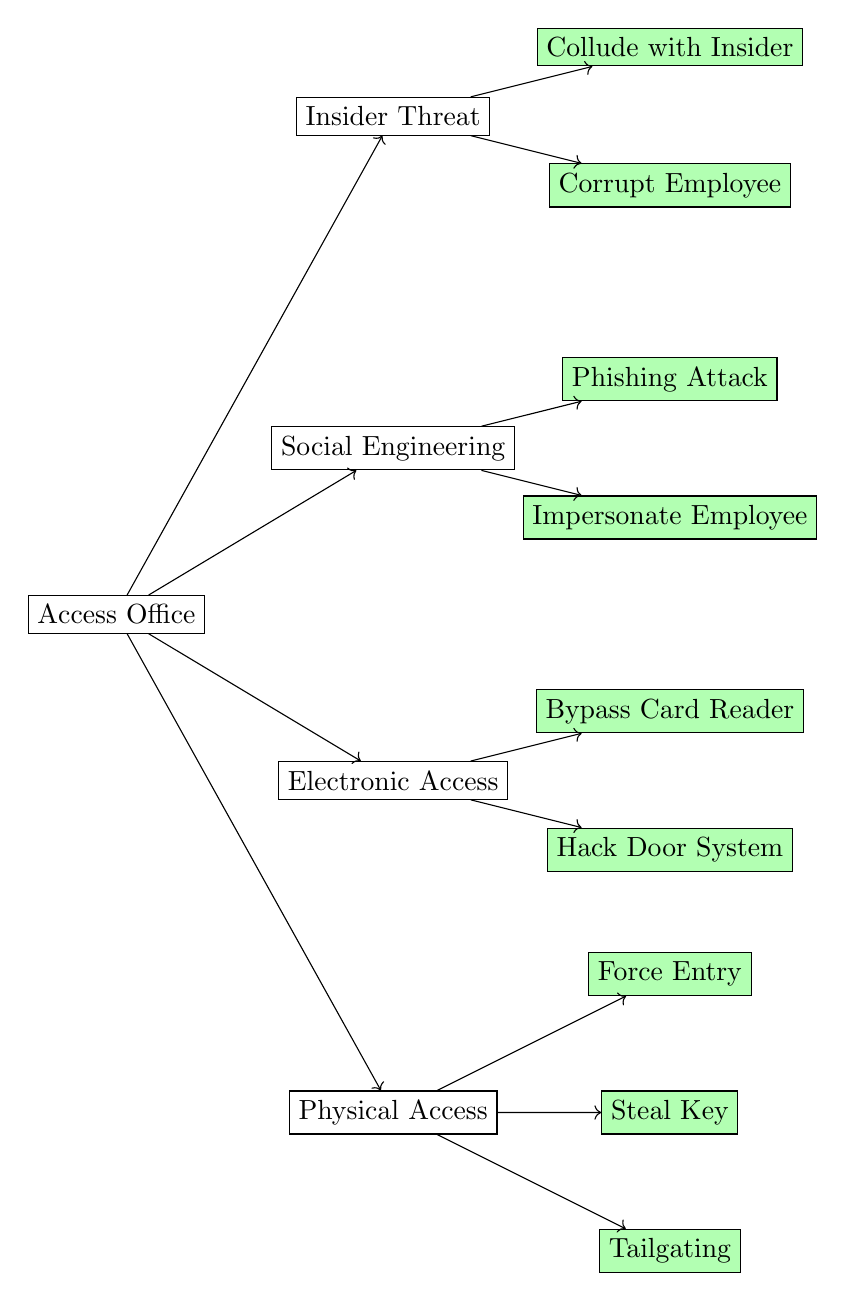
\begin{tikzpicture}[
                                        every node/.style={draw, rectangle, align=center},
                                        grow=east,
                                        sibling distance=12em,
                                        level distance=10em,
                                        level 2/.style={sibling distance=5em},
                                        level 3/.style={sibling distance=2em},
                                        edge from parent/.style={->, draw},
                                        leaf/.style={fill=green!30}
                                        ]
                                      
                                        \node {Access Office}
                                          child { node {Physical Access}
                                            child { node[leaf] {Tailgating} }
                                            child { node[leaf] {Steal Key} }
                                            child { node[leaf] {Force Entry} }
                                          }
                                          child { node {Electronic Access}
                                            child { node[leaf] {Hack Door System} }
                                            child { node[leaf] {Bypass Card Reader} }
                                          }
                                          child { node {Social Engineering}
                                            child { node[leaf] {Impersonate Employee} }
                                            child { node[leaf] {Phishing Attack} }
                                          }
                                          child { node {Insider Threat}
                                            child { node[leaf] {Corrupt Employee} }
                                            child { node[leaf] {Collude with Insider} }
                                          };
                                      
                                      \end{tikzpicture}
                            \subsubsection{Exercise 2}
                            \subparagraph{Question}

                                \( H() \) is a cryptographic hash function that maps a message of an arbitrary bit length onto a 20-bit hash value.

                                \begin{enumerate}
                                    \item[(a)] How many random messages would be required to find two different messages \( M \) and \( M' \) such that \( H(M) = H(M') \)?
                                    \item[(b)] What is the probability that none of \( n \) randomly generated messages collide?
                                \end{enumerate}

                            \subparagraph{Answer}
                            Given that \( H \) is a cryptographic hash function that maps messages to a 20-bit hash value, we have the following points to consider:

                            1. \textbf{Size of the hash output}: A 20-bit hash value means there are \( 2^{20} \) possible hash values.
                            2. \textbf{Birthday problem context}: To find the number of random messages required to find two different messages \( M \) and \( M' \) such that \( H(M) = H(M') \), we can use the birthday paradox.
                            
                             Part (a): Number of random messages required to find a collision
                            
                            The birthday paradox states that for a hash function producing \( n \) possible values, the approximate number of messages \( k \) required to find a collision (i.e., two messages with the same hash value) can be estimated by:
                            
                            \[ k \approx \sqrt{2n} \]
                            
                            For our 20-bit hash function, \( n = 2^{20} \). Plugging this value in:
                            
                            \[ k \approx \sqrt{2 \times 2^{20}} = \sqrt{2^{21}} = 2^{10.5} \approx 2^{10} \times \sqrt{2} \approx 1024 \times 1.414 \approx 1448 \]
                            
                            So, approximately \textbf{1448} random messages would be required to find a collision.
                            
                            Part (b): Probability that none of \( n \) randomly generated messages collide
                            
                            To find the probability that none of \( n \) randomly generated messages collide, we need to calculate the probability that all \( n \) hash values are unique.
                            
                            The total number of possible hash values is \( 2^{20} \).
                            
                            For the first message, there are \( 2^{20} \) possible hash values, and the probability of it being unique is 1 (since there are no other messages yet).
                            
                            For the second message, there are \( 2^{20} - 1 \) possible unique hash values left. Therefore, the probability that the second message does not collide with the first one is:
                            
                            \[ \frac{2^{20} - 1}{2^{20}} \]
                            
                            For the third message, there are \( 2^{20} - 2 \) possible unique hash values left. The probability that the third message does not collide with the first two is:
                            
                            \[ \frac{2^{20} - 2}{2^{20}} \]
                            
                            Continuing this pattern, the probability that none of the \( n \) messages collide is:
                            
                            \[ P(\text{no collisions}) = \frac{2^{20}}{2^{20}} \times \frac{2^{20} - 1}{2^{20}} \times \frac{2^{20} - 2}{2^{20}} \times \ldots \times \frac{2^{20} - (n - 1)}{2^{20}} \]
                            
                            This can be simplified as:
                            
                            \[ P(\text{no collisions}) = \prod_{i=0}^{n-1} \left(1 - \frac{i}{2^{20}}\right) \]
                            
                            For large \( n \), this product can be approximated using the exponential function \( e \):
                            
                            \[ P(\text{no collisions}) \approx \exp\left(-\frac{n(n-1)}{2 \times 2^{20}}\right) \]
                            
                            This approximation is derived from the fact that:
                            
                            \[ \prod_{i=0}^{n-1} \left(1 - \frac{i}{2^{20}}\right) \approx \exp\left(-\sum_{i=0}^{n-1} \frac{i}{2^{20}}\right) \]
                            
                            And the sum of the first \( n-1 \) integers is approximately \( \frac{n(n-1)}{2} \).
                            
                            So, the probability that none of the \( n \) messages collide is:
                            
                            \[ P(\text{no collisions}) \approx \exp\left(-\frac{n^2}{2 \times 2^{20}}\right) \]

                            \subsubsection{Exercise 3}
                                \subparagraph{Question}
                                Alice and Bob are organizing a dinner. Alice is cooking at home and Bob is buying food. To enforce the security in her communications, Alice is appending to her messages a MAC.
                                However, Alice doesn’t expect that her messages can be overheard and tampered with by Eve.
                                Alice sends Bob the message \( M = \text{``buy a gallon of water''} \), with the message authentication code MAC(K,M).
                                
                                \begin{enumerate}
                                    \item Eve intercepts the message and sends to Bob a copy of the same message. How much water will Bob buy? Explain why.
                                    \item Eve intercepts the message and changes ``water'' with ``wine''… will Alice and Bob get drunk tonight?
                                    \item Bob likes beer very much, so he buys beer instead of water and he pretends that the message was \( M' = \text{``buy a gallon of beer''} \). Is Alice able to prove that the message has been forged by Bob?
                                \end{enumerate}
                                
                                \subparagraph{Answer}
                                \begin{enumerate}
                                    \item Bob will buy a gallon of water, because Eve has sent same message so it hasn't been altered.
                                    \item No, they won't get drunk because if Eve has changed the message also MAC is changed so Bob can check it.
                                    \item No, Alice can prove only that the message has been altered, but not who has modified it.  
                                \end{enumerate}
                            \subsubsection{Exercise 4}
                                \subparagraph{Question}
                                Same as before, but this time Alice is using a digital signature:

                                Alice and Bob are organizing a dinner. Alice is cooking at home and Bob is buying food. To enforce the security in her communications, Alice is appending to her messages her digital signature computed with her private key \( K_A \).
                                However, Alice doesn’t expect that her messages can be overheard and tampered with by Eve.
                                Alice sends Bob the message \( M = \text{``buy a gallon of water''} \), with the digital signature \( DS(M,K_A) \).
                                
                                \begin{enumerate}
                                    \item Eve intercepts the message and sends to Bob a copy of the same message. How much water will Bob buy? Explain why.
                                    \item Eve intercepts the message and changes ``water'' with ``wine''… will Alice and Bob get drunk tonight?
                                    \item Bob likes beer very much, so he buys beer instead of water and he pretends that the message was \( M' = \text{``buy a gallon of beer''} \). Is Alice able to prove that the message has/has not been forged by Bob?
                                \end{enumerate}
                                \subparagraph{Answer}
                                 \begin{enumerate}
                                    \item Bob will buy a gallon of water, because Eve has sent same message so it hasn't been altered.
                                    \item No, they won't get drunk because Bob is able to check that who has sent the message isn't Alice and this checking the digital signature which isn't the same of orginal message. 
                                    \item Yes, Alice can prove that the new message has been forged by Bob, because if the signature has been created by Bob, he would have used his own private key, and it will not match Alice's digital signature. 
                                 \end{enumerate}
                                 \newpage
\section{User Identification}
        \subsection{Introduction}
                \subsubsection{Two functions for user authentication}
                \begin{enumerate}
                    \item User identification
                    \begin{itemize}
                        \item by means of a credential or an ID provided by the user to the system
                    \end{itemize}
                    \item User verification
                    \begin{itemize}
                        \item by the exchange of authentication information
                        \item establishes the validity of the claim
                    \end{itemize}
                \end{enumerate}
                \paragraph{Digital
                Authentication
                Guideline} NIST SP 800-63-3 defines digital user
                authentication as (October 2016) :
                “\textit{The process of establishing confidence in user
                identities that are presented electronically to an
                information system.}”
                \paragraph{Identification
                and
                authentication
                security
                requirements}

                \subparagraph{Basic Security Requirements (NIST SP 800-171):}
                \begin{enumerate}
                    \item Identify users, processes acting on behalf of users, or devices.
                    \item Authenticate (or verify) the identities of those users, processes, or devices
                    \begin{itemize}
                        \item prerequisite to allowing access to organizational information systems.
                    \end{itemize}
                \end{enumerate}

                \subparagraph{Derived Security Requirements:}
                \begin{enumerate}
                    \item Use multifactor authentication for local and network access to privileged accounts and for network access to non-privileged accounts.
                    \item Employ replay-resistant authentication mechanisms for network access to all accounts.
                    \item Prevent reuse of identifiers for a defined period.
                    \item Disable identifiers after a defined period of inactivity.
                    \item Enforce a minimum password complexity and change of characters when new passwords are created.
                    \item Prohibit password reuse for a specified number of generations.
                    \item Allow temporary password use for system logons with an immediate change to a permanent password.
                    \item Store and transmit only cryptographically-protected passwords.
                    \item Obscure feedback of authentication information.
                \end{enumerate}

                \begin{figure}[h]
                    \begin{center}
                        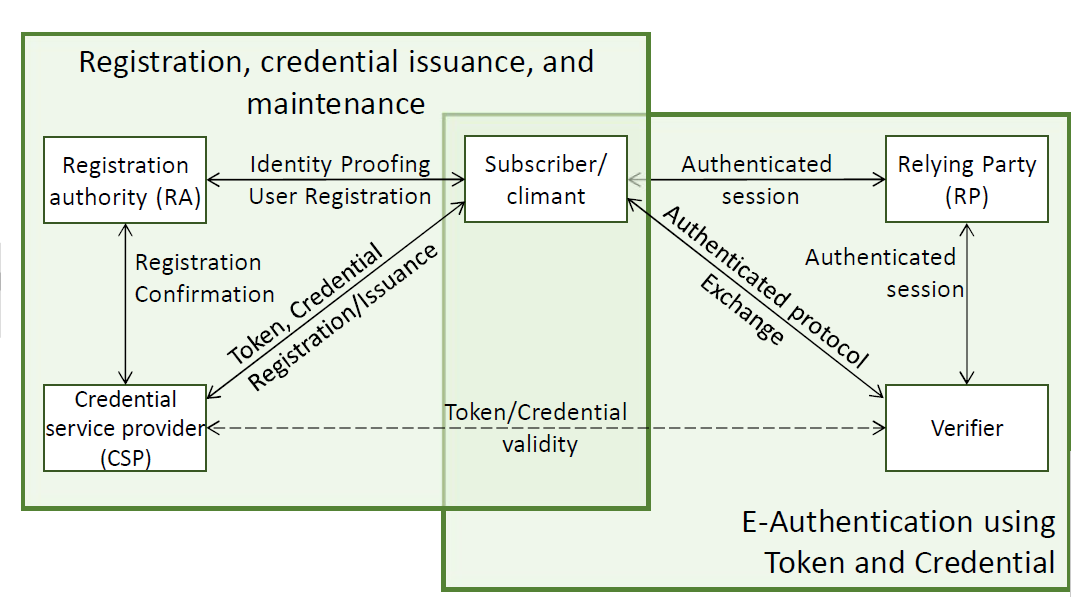
\includegraphics[scale=0.5]{../immagini/Authentication_Model.png}
                    \end{center}
                    \caption{The NIST SP 800-63-3 E-authentication architectural model}
                \end{figure}

                
                \paragraph{Four means of authenticating user identity}
                \begin{itemize}
                    \item Something the individual knows
                    \begin{itemize}
                        \item Password, PIN, answers to prearranged questions
                    \end{itemize}
                    \item Something the individual possesses (token)
                    \begin{itemize}
                        \item Smartcard, electronic keycard, physical key
                    \end{itemize}
                    \item Something the individual is (static biometrics)
                    \begin{itemize}
                        \item Fingerprint, retina, face
                    \end{itemize}
                    \item Something the individual does (dynamic biometrics)
                    \begin{itemize}
                        \item Voice pattern, handwriting, typing rhythm
                    \end{itemize}
                \end{itemize}
                
                \begin{figure}[h]
                    \begin{center}
                        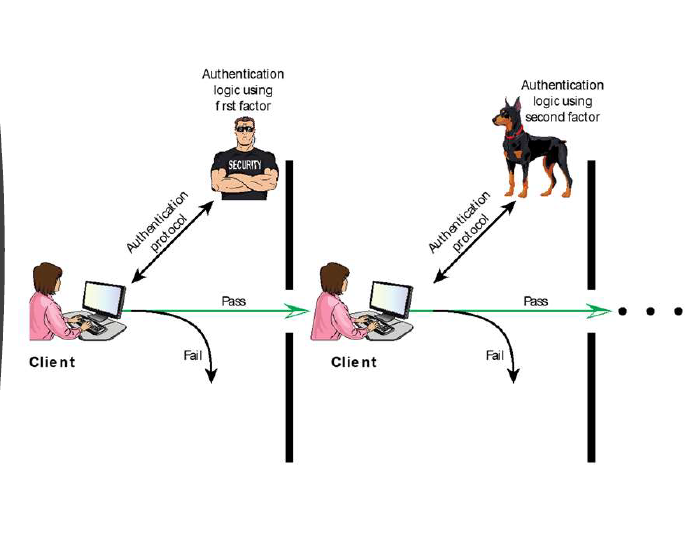
\includegraphics[scale=0.8]{../immagini/Multifactor_Authentication.png}
                    \end{center}
                    \caption{Multifactor
                    authentication}
                \end{figure}
            
                \paragraph{Risk
                assessment
                for user
                authentication}
                    \subparagraph{Assurance level}
                    Describes an
                    organization’s
                    degree of
                    certainty that a
                    user has
                    presented a
                    credential that
                    refers to his or
                    her identity. \\
                    This degree is defined as:
                        \begin{itemize}
                            \item The degree of confidence in the vetting process used to establish the identity of the individual to whom the credential was issued
                            \item The degree of confidence that the individual who uses the credential is the individual to whom the credential was issued
                        \end{itemize}

                    \subparagraph{Potential
                    impact}

                    FIPS 199 defines three levels of potential
                    impact on organizations or individuals should
                    there be a breach of security:

                    \begin{itemize}
                        \item Low
                        \begin{itemize}
                            \item An authentication error could be expected to have a limited adverse effect on organizational operations, organizational assets, or individuals
                        \end{itemize}
                        \item Moderate
                        \begin{itemize}
                            \item An authentication error could be expected to have a serious adverse effect
                        \end{itemize}
                        \item High
                        \begin{itemize}
                            \item An authentication error could be expected to have a severe or catastrophic adverse effect
                        \end{itemize}
                    \end{itemize}
                    \subparagraph{Areas of risk}
                    Maximum potential impact for each   assurance level
                        \begin{table}[h!]
                            \centering
                            \begin{tabular}{|m{7cm}|c|c|c|c|}
                                \hline
                                                                                                & \multicolumn{4}{|c|}{Assurance Level Impact Profiles}\\
                                \hline
                                \textbf{Potential Impact Categories for Authentication Errors} & \textbf{1} & \textbf{2} & \textbf{3} & \textbf{4} \\
                                \hline
                                Inconvenience, distress, or damage to standing or reputation & Low & Mod & Mod & High \\
                                \hline
                                Financial loss or organization liability & Low & Mod & Mod & High \\
                                \hline
                                Harm to organization programs or interests & None & Low & Mod & High \\
                                \hline
                                Unauthorized release of sensitive information & None & Low & Mod & High \\
                                \hline
                                Personal safety & None & None & Low & Mod/High \\
                                \hline
                                Civil or criminal violations & None & Low & Mod & High \\
                                \hline
                            \end{tabular}
                            \caption{Assurance Level Impact Profiles}
                    \end{table}
                    \newpage
                \subsubsection{Question \& Example}
                    \subparagraph{Question:}
                    REFERRING TO THE NIST SP 800-63-3 MODEL, DID YOU EVER
                    EXPERIENCE A CASE OF AUTHENTICATION THAT FOLLOWS THAT
                    MODEL?
                    DESCRIBE THAT AUTHENTICATION SYSTEM FROM THE USER
                    PERSPECTIVE.
                    \subparagraph{Answers:}
                    Yes, I have experienced an authentication system that follows the NIST SP 800-63-3 model. The system is designed to ensure secure and reliable authentication processes. Below is a description of the authentication system from the user's perspective:

                    \begin{itemize}
                        \item \textbf{Initial Registration:}
                        \begin{itemize}
                            \item The user begins by visiting the service's registration page.
                            \item The user is required to provide personal information, such as full name, email address, and phone number.
                            \item The user sets a password that meets the specified complexity requirements.
                            \item The system sends a verification email to the provided email address. The user must click on the link in the email to verify their email address.
                            \item Optionally, the user may be asked to provide additional identity proofing documents or answer knowledge-based questions for higher assurance levels.
                        \end{itemize}
                        
                        \item \textbf{Authentication:}
                        \begin{itemize}
                            \item The user navigates to the login page of the service.
                            \item The user enters their username (or email) and password.
                            \item For multi-factor authentication (MFA), the user is prompted to enter a code sent to their registered phone number via SMS, or to approve the login attempt using an authentication app.
                            \item Upon successful verification of the provided factors, the user is granted access to their account.
                        \end{itemize}
                        
                        \item \textbf{Session Management:}
                        \begin{itemize}
                            \item Once authenticated, the user can manage their session and perform actions within their account.
                            \item The system may prompt the user to re-authenticate for sensitive actions, such as changing account settings or accessing personal data.
                        \end{itemize}
                        
                        \item \textbf{Account Recovery:}
                        \begin{itemize}
                            \item If the user forgets their password, they can initiate a password recovery process.
                            \item The system sends a password reset link to the user's registered email address.
                            \item The user clicks the link and follows the instructions to set a new password.
                            \item Additional verification steps, such as answering security questions or using MFA, may be required to complete the password reset process.
                        \end{itemize}
                        
                        \item \textbf{Periodic Verification:}
                        \begin{itemize}
                            \item Periodically, the system may prompt the user to re-verify their email address and phone number to ensure the information is current.
                            \item The user may also be required to review and update their security settings.
                        \end{itemize}
                    \end{itemize}
                    
                    This multi-layered approach to authentication, incorporating both knowledge-based and possession-based factors, aligns with the NIST SP 800-63-3 guidelines to provide a high level of assurance in the authentication process.
        \subsection{Password-Based Authentication}
        \begin{itemize}
            \item Widely used line of defense against intruders
            \begin{itemize}
                \item User provides name/login and password
                \item System compares password with the one stored for that specified login
            \end{itemize}
            \item The user ID:
                \begin{itemize}
                    \item Determines that the user is authorized to access the system
                    \item Determines the user’s privileges
                    \item Is used in discretionary access control
                \end{itemize}          
        \end{itemize}

        \begin{figure}[h]
            \begin{center}
                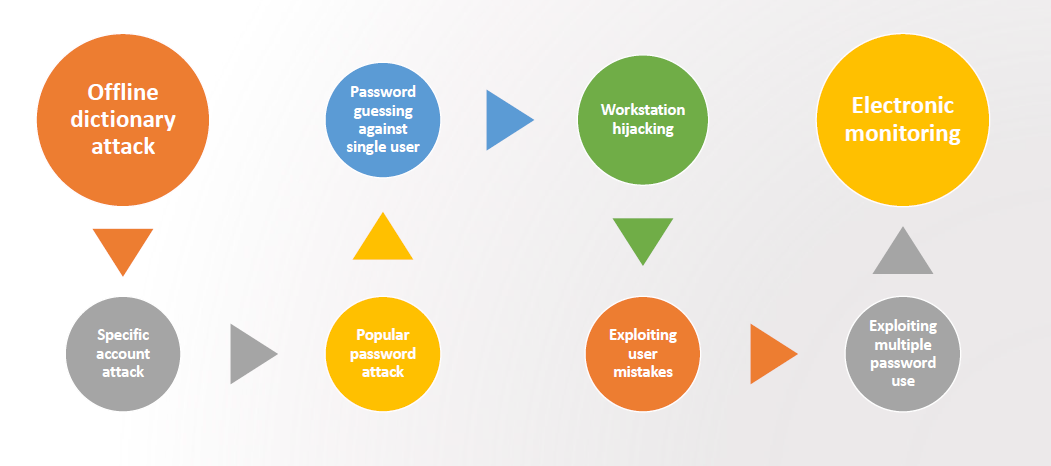
\includegraphics[scale=0.6]{../immagini/password_vulnerabelities.png}
            \end{center}
            \caption{Password Vulnerabilities}
        \end{figure}
        
        \subsubsection{Unix Implementation}
        \begin{figure}[h]
            \begin{center}
                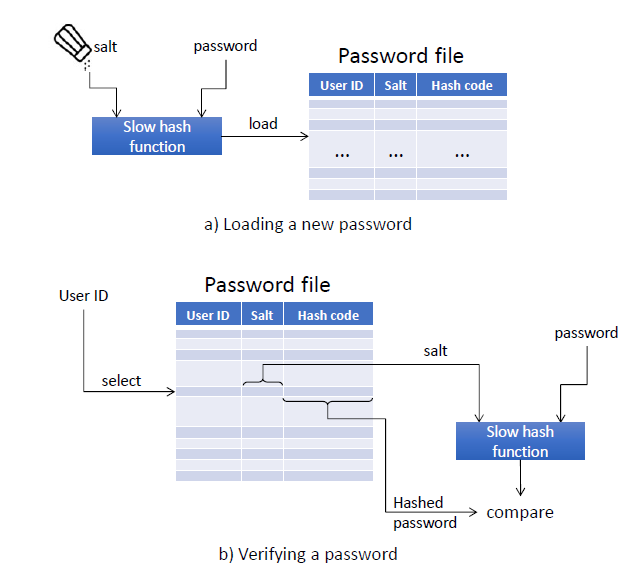
\includegraphics{../immagini/unix_scheme.png}
            \end{center}
            \caption{Unix Scheme}
        \end{figure}

        
         The salt serves three purposes:
            \begin{itemize}
                \item It prevents duplicate passwords from being visible in the password file.
                \item It becomes nearly impossible to find out whether a person with passwords on two or more systems has used the same password on all of them.
                \item It greatly increases the difficulty of offline dictionary attacks.
                \begin{itemize}
                    \item Say the attacker obtains a copy of the password file and salt is not used
                    \begin{itemize}
                        \item … and its goal is to guess a single password of any user.
                    \end{itemize}    
                    \item The attacker may submit a large number of likely passwords to the hashing function:
                        \begin{itemize}
                            \item If any of the guesses matches one of the hashes in the file, then the attacker has found a password that is in the file.
                        \end{itemize}
                    \item Using salt instead, the attacker must take each guess and submit it to the hash function once for each salt value in the dictionary file, multiplying the number of guesses that must be checked.

                \end{itemize}
            \end{itemize}

            \paragraph{Implementation}
                \subparagraph{Original Scheme}
                \begin{itemize}
                    \item Up to eight printable characters in length
                    \item 12-bit salt used to modify DES encryption into a one-way hash function
                    \item Repeatedly encrypted 25 times
                    \item Output translated to 11 character sequence
                \end{itemize}

                Now regarded as inadequate still often required for compatibility with
                existing account management software or
                multivendor environments
                \subparagraph{Improved implementations}

                    \begin{enumerate}
                        \item Much stronger hash/salt schemes available for Unix
                        \item Recommended hash function is based on MD5
                        \begin{itemize}
                            \item Salt of up to 48-bits
                            \item Password length is unlimited
                            \item Produces 128-bit hash
                            \item Uses an inner loop with 1000 iterations to achieve slowdown
                        \end{itemize}
                        \item OpenBSD uses Blowfish block cipher-based hash algorithm called Bcrypt
                            \begin{itemize}
                                \item Most secure version of Unix hash/salt scheme
                                \item Uses 128-bit salt to create 192-bit hash value
                            \end{itemize}
                       
                    \end{enumerate}
        \subsubsection{Password Cracking}
        \begin{itemize}
            \item Dictionary attacks
            \begin{itemize}
                \item Develop a large dictionary of possible passwords and try each against the password file
                \item Each password must be hashed using each salt value and then compared to stored hash values
            \end{itemize}
            \item Rainbow table attacks
            \begin{itemize}
                \item Pre-compute tables of hash values of passwords in dictionary for all salts
                \item A mammoth table of hash values
                \item Can be countered by using a sufficiently large salt value and a sufficiently large hash length
            \end{itemize}
            \item Password crackers exploit the fact that people choose easily guessable passwords
            \begin{itemize}
                \item Shorter password lengths are also easier to crack
            \end{itemize}
            \item John the Ripper
            \begin{itemize}
                \item Open-source password cracker first developed in 1996
                \item Uses a combination of brute-force and dictionary techniques
            \end{itemize}
        \end{itemize}

            \paragraph{Modern Approaches}
            \begin{itemize}
                \item Complex password policy
                \begin{itemize}
                    \item Forcing users to pick stronger passwords
                \end{itemize}
                \item However, password-cracking techniques have also improved
                \begin{itemize}
                   \item The processing capacity available for password cracking has increased dramatically
                    \item The use of sophisticated algorithms to generate potential passwords
                    \item Studying examples and structures of actual passwords in use
                \end{itemize}
            \end{itemize}
            
            \begin{figure}[h]
                \begin{center}
                    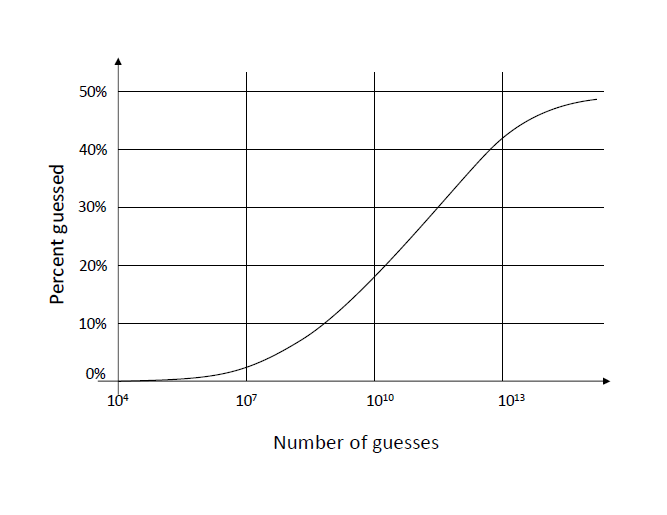
\includegraphics{../immagini/percentage1.png}
                \end{center}
                \caption{Percentage of
                passwords
                guess after a
                given number
                of guesses}
            \end{figure}

            \paragraph{Password file
            access control}
                    Can block offline guessing attacks by denying access to
                    encrypted passwords
                    \begin{itemize}
                        \item Make available only to privileged users
                        \item Shadow Password File
                    \end{itemize}

                    \subparagraph{Vulnerabilities}
                    \begin{itemize}
                        \item Weakness in the OS that allows access to the file
                        \item Accident with permissions making it readable
                        \item Users with same password on other systems
                        \item Access from backup media
                        \item Sniff passwords in network traffic
                    \end{itemize}
            \paragraph{Password selection strategies}
                    
                        \begin{enumerate}
                            \item User education:
                            \begin{itemize}
                                \item Users can be told the importance of using hard to guess passwords and can be provided with guidelines for selecting strong passwords.
                            \end{itemize}
                            \item Computer generated passwords:
                            \begin{itemize}
                                \item Users have trouble remembering them.
                            \end{itemize}
                            \item Reactive password checking:
                            \begin{itemize}
                                \item System periodically runs its own password cracker to find guessable passwords.
                            \end{itemize}
                            \item Complex password policy:
                            \begin{itemize}
                                \item User is allowed to select his own password, but the system checks if the password is allowable. If not, rejects it.
                                \item Goal is to eliminate guessable passwords while allowing the user to select a password easy to remember.
                            \end{itemize}
                        \end{enumerate}
            \paragraph{Proactive password checking}
                    \begin{enumerate}
                        \item Rule enforcement:
                        \begin{itemize}
                            \item Specific rules that passwords must adhere to
                        \end{itemize}    
                        \item Password checker
                            \begin{itemize}
                                \item Compile a large dictionary of “bad” passwords not to use
                            \end{itemize}
                        \item But how to make a fast password check?
                            \begin{itemize}
                                \item Bloom filter, used to implement password checkers
                            \begin{itemize}
                                \item Exploits k hash functions to build tables of hash values
                                \item Check desired password against this table
                                \item It’s a probabilistic, efficient way to check if a password is in the dictionary of forbidden passwords
                            \end{itemize} 
                            \end{itemize}
                            
                        
                    \end{enumerate}
                    \subparagraph{Bloom filter password checker:}
                    Bloom filter constructed over a dictionary \( \mathcal{D} \) of passwords... say that:
                    \begin{itemize}
                        \item \( \mathcal{D} = \{ d_1, d_2, \ldots, d_m \} \)
                        \item \( h_1, h_2, \ldots, h_k \) are hash functions, where \( h_i: \mathcal{D} \to [0, n-1] \)
                        \item Bloom filter \( \mathcal{B} \) is an array of \( n \) bits
                    \end{itemize}
                    
                    Bloom filter constructed as:
                  
                   \[
                    \begin{aligned}
                    & \text{Let } \mathcal{B}[i] = 0 \text{ for each } i \in 0, 1, \ldots, n-1:\\                
                    & \text{For each } x \in \mathcal{D}:\\
                    & \qquad \text{For each } j \in 1, 2, \ldots, k: \quad \mathcal{B}[h_j(x)] = 1
                    \end{aligned}
                    \]

                    To check a password \( y \) with the Bloom filter:
             
                                            
                    \[
                    \begin{aligned}
                    & \text{if } \mathcal{B}[h_j(y)] = 0 \text{ for some } j \in 1, 2, \ldots, k: \\
                    & \qquad \text{return } \text{valid} \quad // \text{password } y \text{ is not in } \mathcal{D} \\
                    & \text{else:} \\
                    & \qquad \text{return } \text{rejected} \quad // \text{password } y \text{ may be in } \mathcal{D}
                    \end{aligned}
                    \]


                    The Bloom filter does not have false negatives:
                   
                        \textit{If \textbf{valid}, then \( y \) is not present in \( \mathcal{D} \)}
                    

                    The Bloom filter may have false positives:
                    
                        \textit{If \textbf{rejected}, then \( y \) may still not be in \( \mathcal{D} \)}
                       
                        \subparagraph{Example:} \( \mathcal{D} = \{ \text{Stefano}, \text{Paolo} \} \)

                        Say that:
                        \[
                        h_1(\text{Stefano}) = 10; \quad h_2(\text{Stefano}) = 7; \quad h_3(\text{Stefano}) = 3
                        \]
                        \[
                        h_1(\text{Paolo}) = 7; \quad h_2(\text{Paolo}) = 12; \quad h_3(\text{Paolo}) = 1
                        \]
                        
                        Hence \( \mathcal{B} = \)
                        \vspace{10pt}
                        \begin{tabular}{|*{13}{c|}}
                            \hline
                            0 & 1 & 2 & 3 & 4 & 5 & 6 & 7 & 8 & 9 & 10 & 11 & 12 \\
                            \hline
                            0 & 1 & 0 & 1 & 0 & 0 & 0 & 1 & 0 & 0 & 1 & 0 & 1 \\
                            \hline
                        \end{tabular}\\
                        \vspace{10pt}
                            Now, consider passwords \( \text{Rita} \) and \( \text{Sofia} \), and that:
                            \[
                            h_1(\text{Rita}) = 3; \quad h_2(\text{Rita}) = 12; \quad h_3(\text{Rita}) = 1
                            \]
                            \[
                            h_1(\text{Sofia}) = 2; \quad h_2(\text{Sofia}) = 9; \quad h_3(\text{Sofia}) = 7
                            \]
                            Then:
                            \begin{itemize}
                                \item \( \text{Rita} \) is rejected
                                \item \( \text{Sofia} \) is valid
                            \end{itemize}

                            \vspace*{10pt}
                            Need to find a proper configuration of the parameters (values of k, m, n), else the mechanism may be unusable
                            it may give too many false positives
                \subsubsection{Question \& Examples}
                            \subparagraph{Question:}
                                                        AN ADVERSARY PERFORMS A BRUTE
                            FORCE ATTACK AND IN 1 YEAR TESTS
                            EXHAUSTIVELY ALL THE POTENTIAL
                            PINS OF A USER.
                            IF THE PINS ARE OF 6 DIGITS, EACH IN
                            AN ALPHABET OF 10 SYMBOLS, HOW
                            LONG IT TAKES TO TEST ONE PIN?
                            \subparagraph{Answer:}
                            \begin{itemize}
                                \item Each PIN is 6 digits long.
                                \item The alphabet for each digit consists of 10 symbols (0-9).
                                \item Therefore, the total number of possible PINs is:
                                \[
                                10^6 = 1,000,000
                                \]
                                \item The adversary tests all 1,000,000 possible PINs in 1 year.
                            
                            \item The duration of 1 year can be converted to seconds as follows:
                                \begin{align*}
                                \text{1 year} &= 365 \, \text{days} \\
                                &= 365 \times 24 \, \text{hours} \\
                                &= 365 \times 24 \times 60 \, \text{minutes} \\
                                &= 365 \times 24 \times 60 \times 60 \, \text{seconds} \\
                                &= 31,536,000 \, \text{seconds}
                                \end{align*}
                            
                            \item The time taken to test one PIN can be calculated by dividing the total time by the number of PINs:
                                \[
                                \text{Time per PIN} = \frac{\text{Total time in seconds}}{\text{Total number of PINs}}
                                \]
                            
                                \[
                                \text{Time per PIN} = \frac{31,536,000 \, \text{seconds}}{1,000,000} \approx 31.536 \, \text{seconds per PIN}
                                \]
                            
                            \end{itemize}
                            
                            Thus, it takes approximately 31.536 seconds to test one PIN.
                  \subsubsection{Question \& Examples}
                            \subparagraph{Question} Comments on the Suitability of Passwords
                            \subparagraph{Answer}:    
                                       
                        \begin{itemize}
                            \item \textbf{Back\#To\#Black\#} \\
                            This password contains a mix of uppercase and lowercase letters, special characters (\#), and has a relatively good length. It is generally considered a strong password due to its complexity and length. However, the repeated pattern of special characters might make it slightly predictable. Overall, it is still a good choice.

                            \item \textbf{09876} \\
                            This password is entirely numeric and only 5 characters long. It is very weak as it can be easily guessed or cracked using brute force attacks. Short numeric passwords are generally not recommended due to their low entropy.

                            \item \textbf{viaFermi3} \\
                            This password contains lowercase letters and a digit, making it moderately strong. It has a reasonable length and includes a mix of characters. However, adding uppercase letters and special characters could further improve its strength.

                            \item \textbf{ketchup} \\
                            This password is a common word and entirely lowercase, making it weak. It lacks complexity and is susceptible to dictionary attacks. Passwords based on common words are not recommended.

                            \item \textbf{onafetS} \\
                            This password contains only letters but has a mix of uppercase and lowercase characters. It is relatively short and could be stronger with the inclusion of digits and special characters. Additionally, it might be a reversal of a common word, which could make it more predictable.

                            \item \textbf{S0Ll3van7e} \\
                            This password is strong as it includes uppercase and lowercase letters, digits, and has a good length. The mix of different character types and its length contribute to higher entropy, making it a good choice for a secure password.
                        \end{itemize}

                    \subparagraph{Question}
                        THE SALT IN THE UNIX PASSWORD SCHEME INCREASES THE
                    DIFFICULTY OF GUESSING BY A FACTOR OF 4096.
                    \begin{enumerate}
                        \item  HOW MANY BITS IS THE SALT?
                        \item  THE SALT IS STORED IN PLAINTEXT IN THE SAME ENTRY AS
                        THE CORRESPONDING CIPHERTEXT PASSWORD.
                        THEREFORE, IT IS KNOWN TO THE ATTACKER AND NEED
                        NOT BE GUESSED. WHY IS IT ASSERTED THAT THE SALT
                        INCREASES SECURITY?
                    \end{enumerate}
                    \subparagraph{Answer}
                    \begin{enumerate}
                        \item The salt is made by 12 bit, that is saved with User ID and Ciphertext Password, that permit to hash result to be more random.
                        \item The salt increases security because ,by changing it , allowed to have different hash result also if password used is the same. 
                    \end{enumerate}
                    \subparagraph{Question}
                    STILL ABOUT SALT:
                    WOULDN’T IT BE POSSIBLE TO THWART COMPLETELY ALL
                    PASSWORD CRACKERS BY DRAMATICALLY INCREASING THE SALT
                    SIZE TO, SAY, 24 OR 48 BITS?
                    \subparagraph{Answer}
                    Increasing the salt size, surelly, we raise password's security, but to thwart completely all password cracker is impossible because there are many techniques that permit to semply also brute force as Dictionary.  
        
        \subsection{Token-Based authentication}
                     Objects that a user possesses for the purpose
                     of user authentication are called tokens: 
                     \begin{itemize}
                      \item  Memory cards
                      \item  Smart tokens/cards
                     \end{itemize}
                    
                 
                        \begin{table}[h]
                            \begin{center}
                                
                            \begin{tabular}{|l|l|l|}
                            \hline
                            \textbf{Card Type}                                                                            & \textbf{Defining Feature}                                                                                                                                                & \textbf{Example}                   \\ \hline
                            Embossed                                                                                      & Raised characters only, on front                                                                                                                                         & Old credit card                    \\ \hline
                            Memory                                                                                        & Electronic memory inside                                                                                                                                                 & Prepaid phone card                 \\ \hline
                            \multirow{3}{*}{\begin{tabular}[c]{@{}l@{}}Smart tokens\\ Contact\\ Contactless\end{tabular}} & \multirow{3}{*}{\begin{tabular}[c]{@{}l@{}}Electronic memory and processor inside\\ Electrical contacts exposed on surface\\ Radio antenna embedded inside\end{tabular}} & \multirow{3}{*}{Biometric ID card} \\
                                                                                                                        &                                                                                                                                                                          &                                    \\
                                                                                                                        &                                                                                                                                                                          &                                    \\ \hline
                            \end{tabular}
                               \end{center}

                            \caption{
                            Types of cards used as tokens}
                            \end{table}

                        \begin{figure}[h]
                            \begin{center}
                                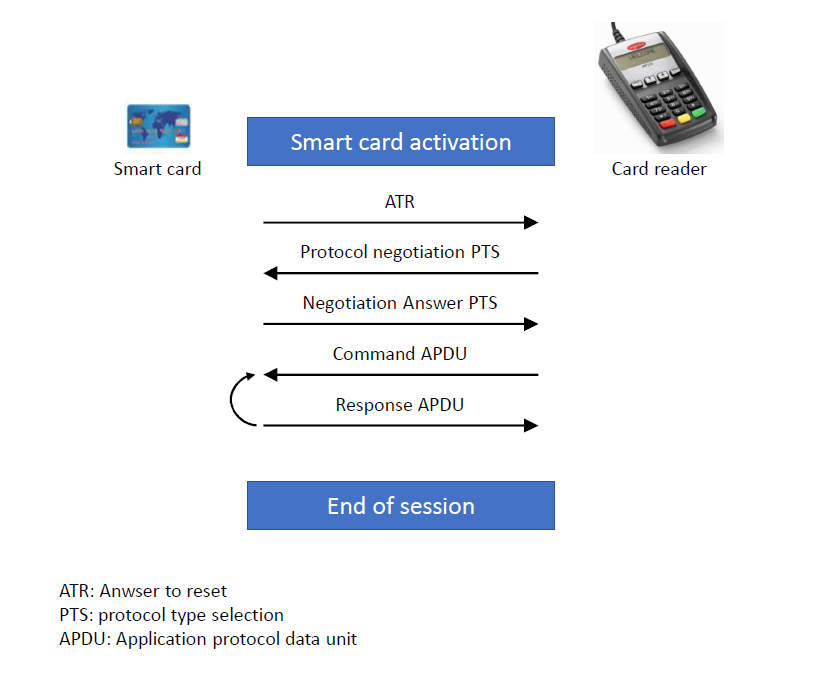
\includegraphics[scale=0.7]{../immagini/smart_card_funciton.png}
                            \end{center}
                            \caption{Smart cart /
                            reader
                            exchange}
                        \end{figure}

                        \subsubsection{Application}
                        \paragraph{Electronic Identity Cards (eID)}
                        Use of a smart card as a national identity card for
                        citizens.
                        Can serve the same purposes as other national ID cards, and
                        similar cards such as a driver’s license, for access to government
                        and commercial services.
                        Can provide stronger proof of identity and can be used in a wider
                        variety of applications.
                        In effect, is a smart card that has been verified by the national
                        government as valid and authentic. An example is the German card neuer
                        Personalausweis. Has human-readable data printed on its surface
                        \begin{itemize}
                            \item Personal data
                            \item Document number
                            \item Card access number (CAN)
                            \item Machine readable zone (MRZ)
                        \end{itemize}



                        \begin{table}[h]
                            \centering
                            \resizebox{\columnwidth}{!}{%
                            \begin{tabular}{|c|c|c|c|c|}
                            \hline
                            \multicolumn{1}{|l|}{\textbf{Function}} &
                            \multicolumn{1}{l|}{\textbf{Purpose}} &
                            \multicolumn{1}{l|}{\textbf{\begin{tabular}[c]{@{}l@{}}PACE\\ Password\end{tabular}}} &
                            \multicolumn{1}{l|}{\textbf{Data}} &
                            \multicolumn{1}{l|}{\textbf{Users}} \\ \hline
                            \begin{tabular}[c]{@{}c@{}}ePass\\ (mandatory)\end{tabular} &
                            \begin{tabular}[c]{@{}c@{}}Authorized offline\\ inspection systems read\\ the data\end{tabular} &
                            CAN or MRZ &
                            \begin{tabular}[c]{@{}c@{}}Face image; two\\ fingerprint images\\ (optional); MRZ data\end{tabular} &
                            \begin{tabular}[c]{@{}c@{}}Offline biometric identity\\ verification reserved for\\ government access\end{tabular} \\ \hline
                            \multirow{2}{*}{\begin{tabular}[c]{@{}c@{}}eID\\ (activation\\ optional)\end{tabular}} &
                            \begin{tabular}[c]{@{}c@{}}Online applications read\\ the data or access\\ functions as authorized.\end{tabular} &
                            eID PIN &
                            \multirow{2}{*}{\begin{tabular}[c]{@{}c@{}}Family and given\\ names; artistic name\\ and doctoral degree:\\ date and place of\\ birth; address and community ID;\\ expiration date\end{tabular}} &
                            \multirow{2}{*}{\begin{tabular}[c]{@{}c@{}}Identification; age\\ verification; community\\ ID verification; restricted\\ identification (pseudonym); revocation\\ query Offline inspection\\ systems read the\end{tabular}} \\ \cline{2-3}
                            &
                            \begin{tabular}[c]{@{}c@{}}Offline inspection\\ systems read the data\\ and update the address\\ and community ID.\end{tabular} &
                            CAN or MRZ &
                            &
                            \\ \hline
                            \multirow{2}{*}{\begin{tabular}[c]{@{}c@{}}eSign\\ (certificate\\ optional)\end{tabular}} &
                            \begin{tabular}[c]{@{}c@{}}A certification authority\\ installs the signature\\ certificate online.\end{tabular} &
                            eID PIN &
                            \multirow{2}{*}{\begin{tabular}[c]{@{}c@{}}Signature key; X.509\\ certificate\end{tabular}} &
                            \multirow{2}{*}{\begin{tabular}[c]{@{}c@{}}Electronic signature\\ Citizens make signature creation\end{tabular}} \\ \cline{2-3}
                            &
                            \begin{tabular}[c]{@{}c@{}}Citizens make signature creation\\ creation electronic\\ signature with eSign PIN.\end{tabular} &
                            CAN &
                            &
                            \\ \hline
                            \end{tabular}%
                            }
                            \caption{Electronic
                            functions for
                            eID cards}
                            \end{table}

                            \begin{description}
                                \item[CAN] card access number
                                \item[MRZ] machine readable zone
                                \item[PACE] password authenticated connection establishment
                                \item[PIN] personal identification number
                            \end{description}


                            \begin{figure}
                                \begin{center}
                                    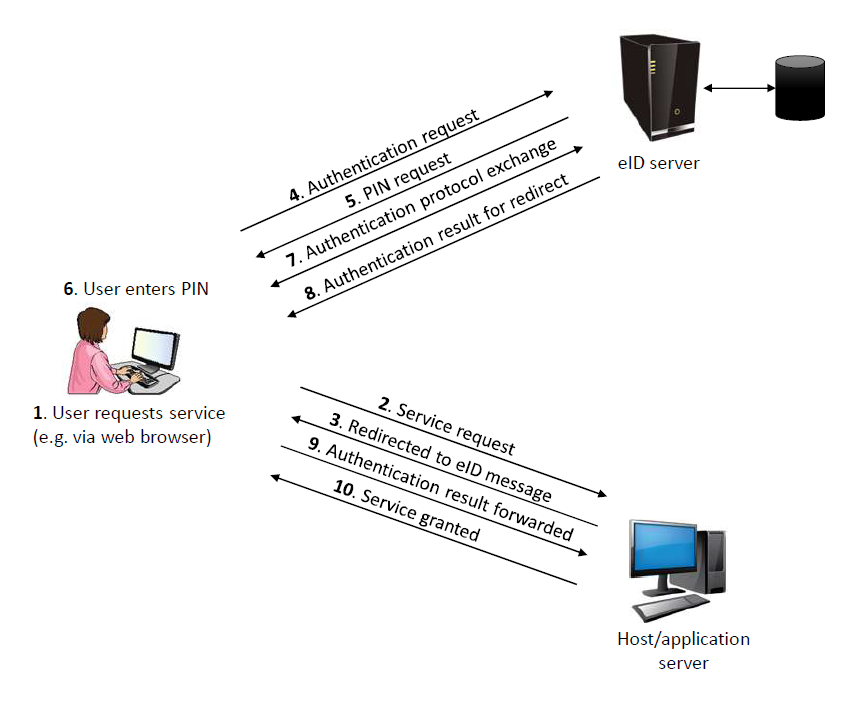
\includegraphics[scale=0.6]{../immagini/user_authentication.png}
                                \end{center}
                                \caption{User
                                authentication
                                with eID}
                            \end{figure}
                            
                            \paragraph{Password Authenticated Connection Establishment}

                            The eID card has a contactless RF chip that is protected by access control measures to ensure it cannot be read without proper authorization.

                            \begin{itemize}
                                \item \textbf{Online applications}: The user must enter a 6-digit PIN, which should only be known to the cardholder.
                                \item \textbf{Offline applications}: Access is granted using either the MRZ (machine-readable zone) printed on the back of the card or the CAN (card access number) printed on the front.
                            \end{itemize}
                            \vspace{10pt}
                            \subparagraph{Explanation:}
                            \begin{itemize}
                                \item \textbf{Contactless RF Chip Protection}: The eID card contains a contactless radio frequency (RF) chip. To protect the data on this chip, explicit access control mechanisms are in place. This means the chip cannot be read unless the correct access protocols are followed.
                                
                                \item \textbf{Online Applications}: When using the eID card for online purposes, the user needs to enter a 6-digit personal identification number (PIN). This PIN acts as a security measure, ensuring that only the person who knows the PIN (presumably the cardholder) can use the card.
                                
                                \item \textbf{Offline Applications}: In scenarios where the eID card is used offline (e.g., at a physical terminal), access to the card's data can be gained by using either:
                                \begin{itemize}
                                    \item The \textbf{MRZ} (machine-readable zone), which is a string of characters printed on the back of the card that can be read by a machine.
                                    \item The \textbf{CAN} (card access number), which is a specific number printed on the front of the card.
                                \end{itemize}
                            \end{itemize}
                \subsection{Biometric Authentication}
                Attempts to authenticate an individual based
                on unique physical characteristics, it is based on pattern recognition and is technically complex and expensive when
                compared to passwords and tokens
                \textbf{Physical characteristics usde include:}
                \begin{itemize}
                    \item Facial characteristics
                    \item Fingerprints
                    \item Hand geometry
                    \item Retinal pattern
                    \item Iris
                    \item Signature
                    \item Voice
                \end{itemize}

                \begin{figure}[h]
                    \begin{center}
                        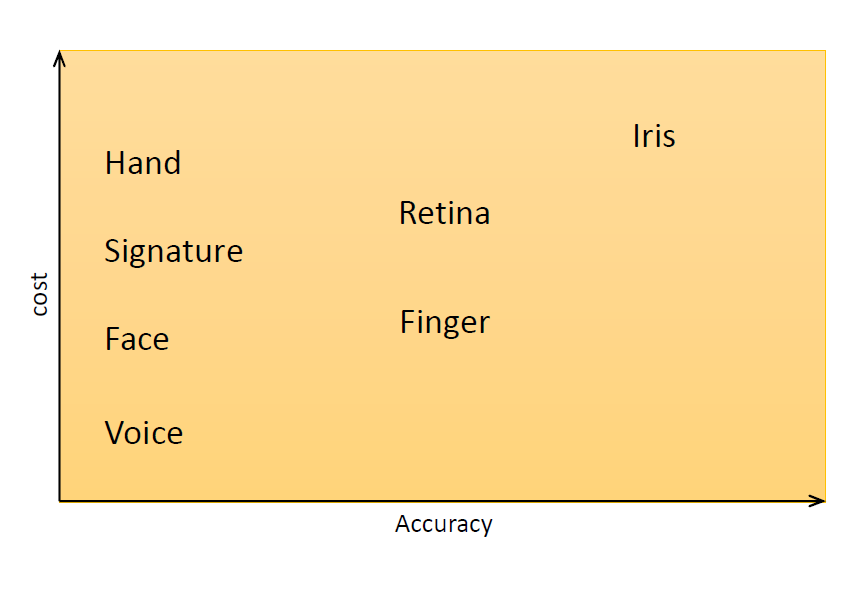
\includegraphics[scale=0.5]{../immagini/cost_accuracy.png}
                    \end{center}
                    \caption{Cost vs
                    accuracy of
                    biometric
                    characteristics
                    in user
                    authentication
                    schemes}
                \end{figure}

                 \begin{figure}[h]
                    \begin{center}
                        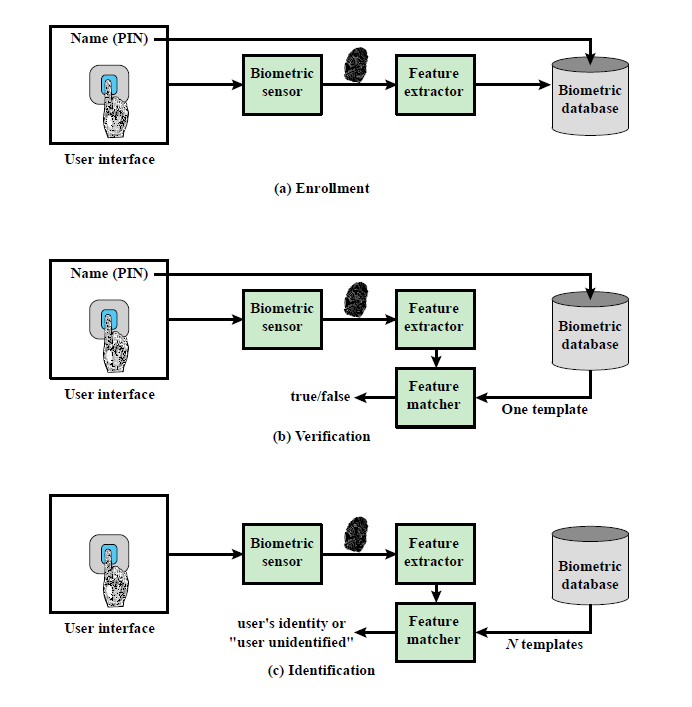
\includegraphics[scale=0.5]{../immagini/Biometric_system.png}
                    \end{center}
                    \caption{A generic
                    biometric
                    system}
                \end{figure}
                \begin{figure}[h]
                    \begin{center}
                        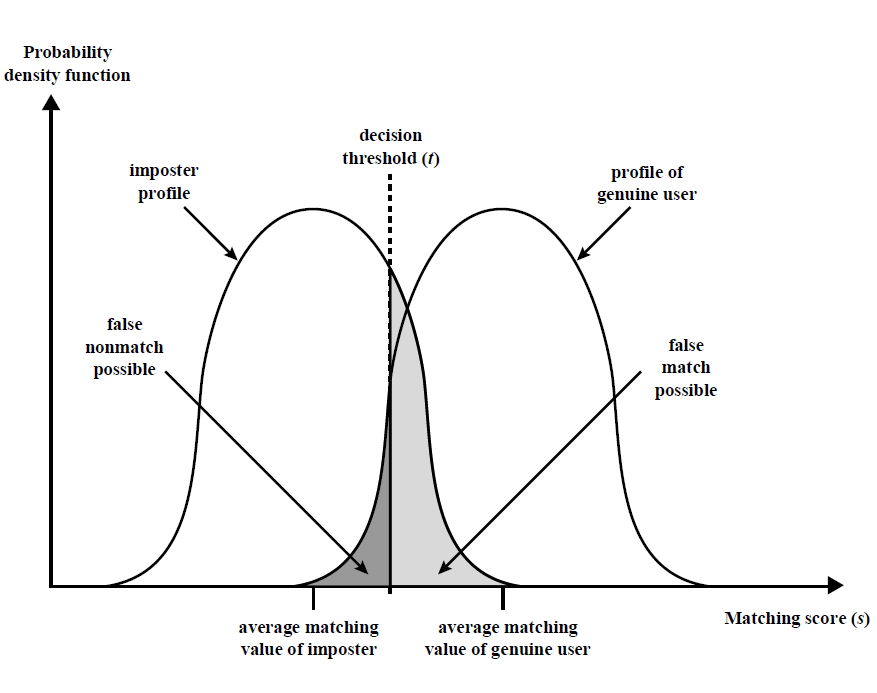
\includegraphics[scale=0.5]{../immagini/Density.png}
                    \end{center}
                    \caption{Profiles of
                    biometric
                    characteristics}
                \end{figure}
                 \begin{figure}[h]
                    \begin{center}
                        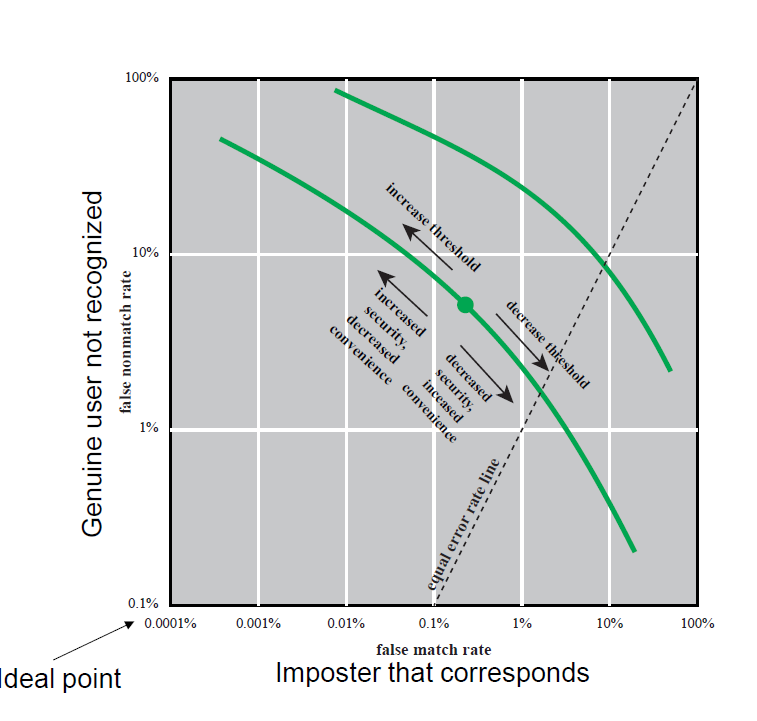
\includegraphics[scale=0.5]{../immagini/Log.png}
                    \end{center}
                    \caption{Idealized
                    biometric
                    measurement
                    operating
                    characteristic
                    curves}
                \end{figure}
                 \begin{figure}[h]
                    \begin{center}
                        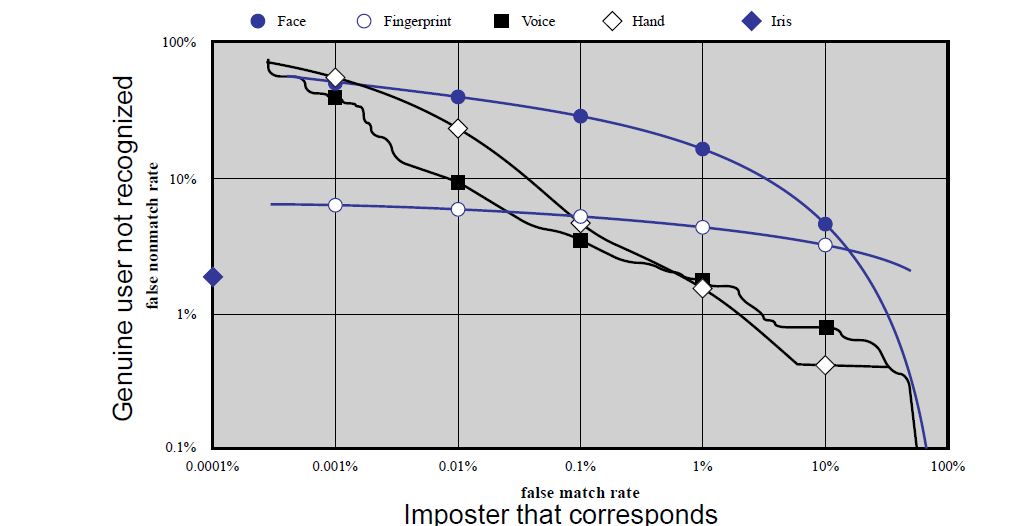
\includegraphics[scale=0.5]{../immagini/BiometriMesaurement.png}
                    \end{center}
                    \caption{Actual biometric measurement operating characteristic
                    curves (log-scale)}
                \end{figure}
                \newpage
            \subsubsection{Question \& Examples}
                \subparagraph{Question:}
                “JANE SPLIT A STONE INTO TWO PIECES, KEPT ONE FOR
                HERSELF, AND GAVE THE OTHER TO JASON. SO SHE SAID -
                WHEN YOU WILL SEND YOUR EMISSARY GIVE HIM THIS HALF
                OF THE STONE AND I WILL RECOGNIZE HIM.”
                WHAT KIND OF AUTHENTICATION IS THIS?
                \subparagraph{Answer}
                This scenario describes a form of \textbf{physical token-based authentication}. In this type of authentication, the possession of a specific physical object (in this case, the matching half of a split stone) is used to verify the identity of an individual. The stone acts as a unique token that is difficult to replicate, ensuring that only someone with the corresponding half of the stone can be authenticated as the legitimate emissary.
            \newpage
            \newpage
                \subsection{Remote User Authentication}
        Authentication over a network, the Internet, or
        a communications link is more complex because there are additional security threats such as:
        \textbf{Eavesdropping, capturing a password, replaying an
        authentication sequence that has been observed} and generally rely on some form of a challengeresponse
        protocol to counter threats. 
        \newpage
            \subsubsection{Basic challengeresponse
                protocol for
                remote user
                authentication}
                \begin{figure}[h]
                    \begin{center}
                        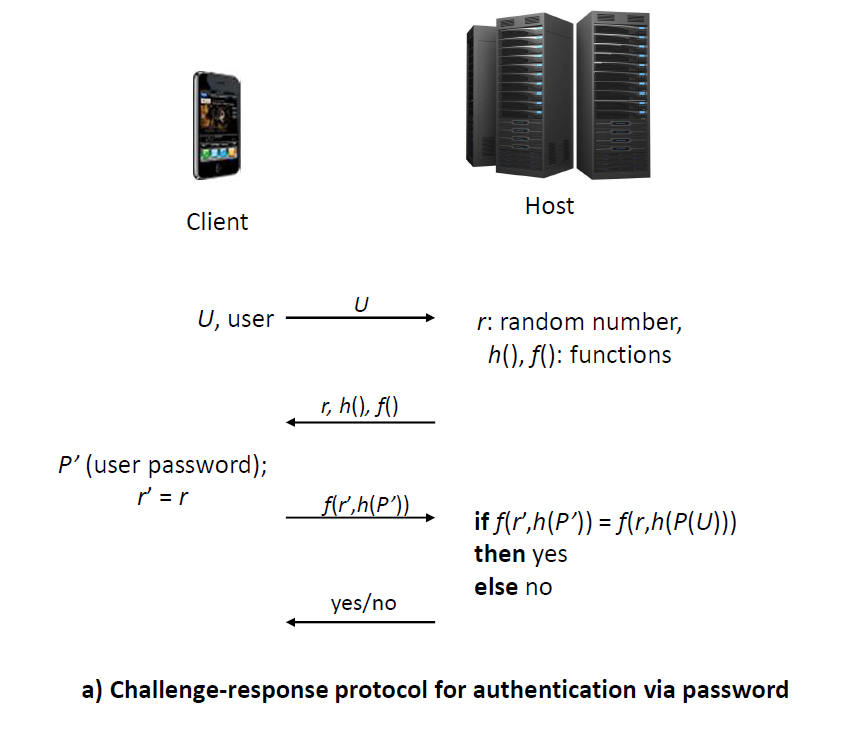
\includegraphics[scale=0.5]{../immagini/network_protocol1.png}
                    \end{center}
                \end{figure}
                \begin{figure}[h]
                    \begin{center}
                        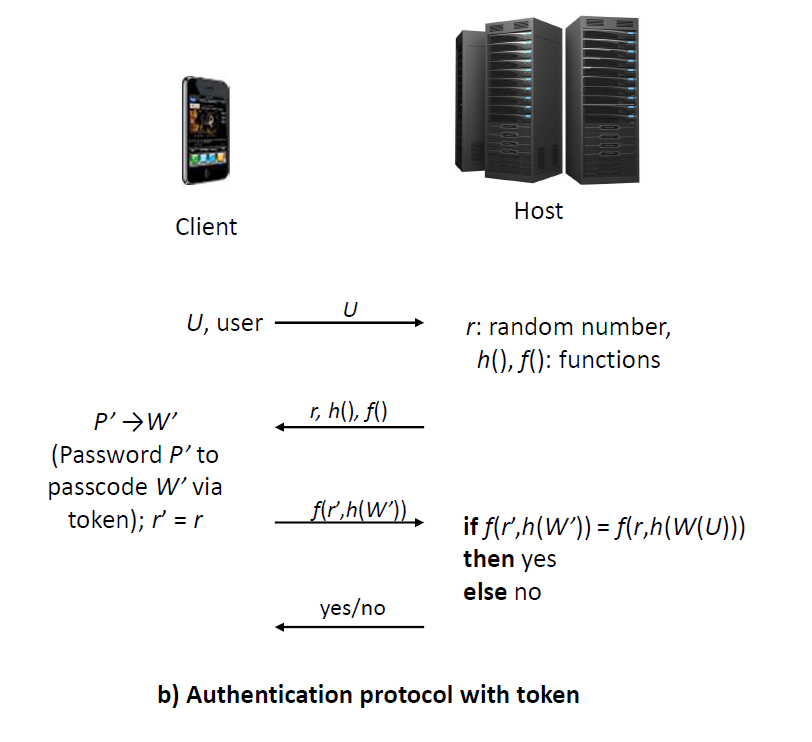
\includegraphics[scale=0.5]{../immagini/network_protocol2.png}
                    \end{center}
                \end{figure}
                \begin{figure}[h]
                    \begin{center}
                        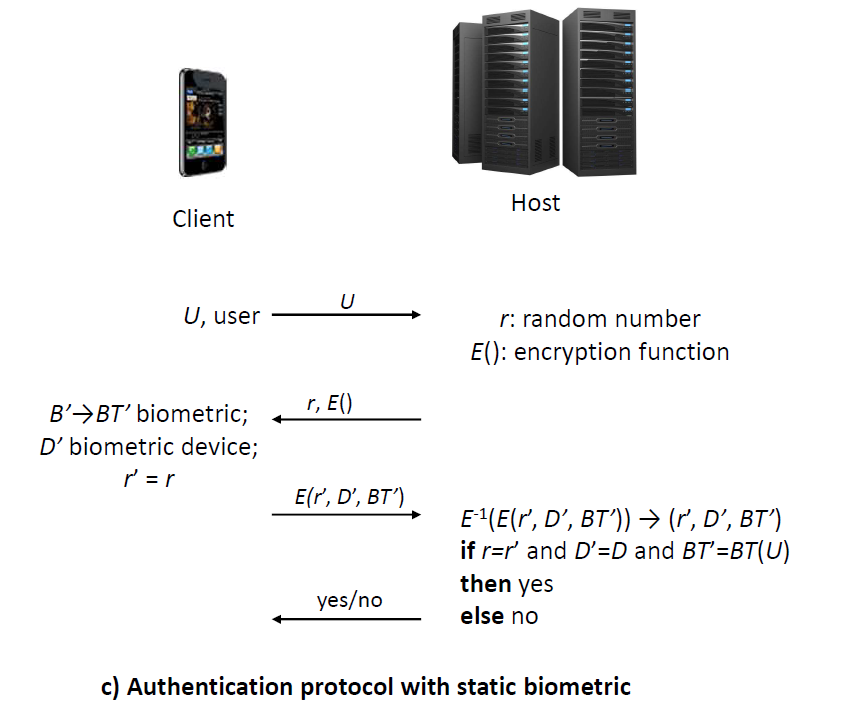
\includegraphics[scale=0.5]{../immagini/network_protocol3.png}
                    \end{center}
                \end{figure}
                \begin{figure}[h]
                    \begin{center}
                        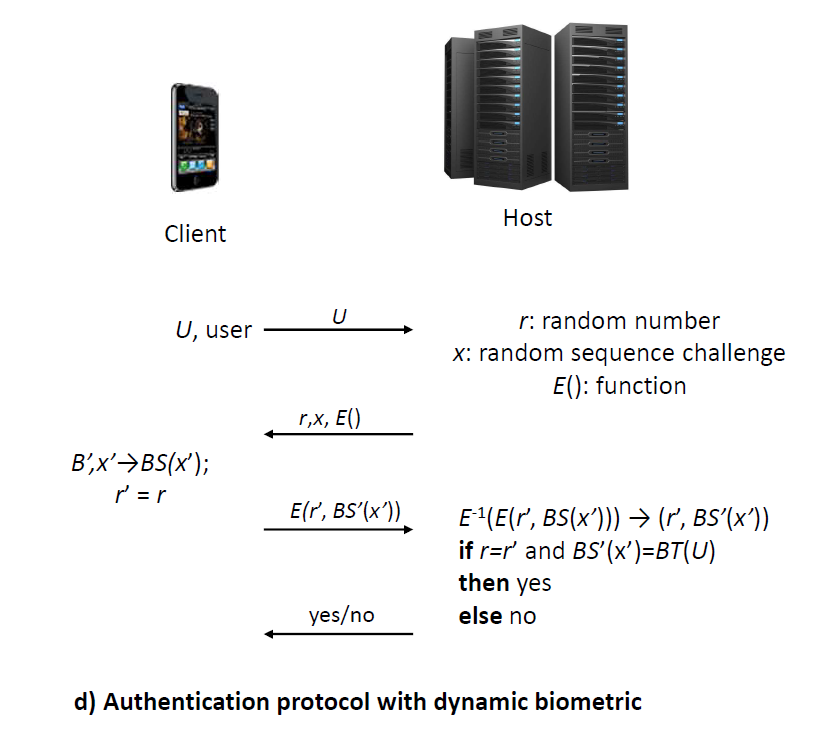
\includegraphics[scale=0.5]{../immagini/network_protocol4.png}
                    \end{center}
                \end{figure}
        \newpage
        \subsubsection{Authentication security issues}
        \begin{description}
            \item[Eavesdropping] 
            Adversary attempts to learn the password by some sort of attack that involves the physical proximity of user and adversary.
        
            \item[Host Attacks] 
            Directed at the user file at the host where passwords, token passcodes, or biometric templates are stored.
        
            \item[Replay] 
            Adversary repeats a previously captured user response.
        
            \item[Client Attacks] 
            Adversary attempts to achieve user authentication without access to the remote host or the intervening communications path.
        
            \item[Trojan Horse] 
            An application or physical device masquerades as an authentic application or device for the purpose of capturing a user password, passcode, or biometric.
        
            \item[Denial-of-Service] 
            Attempts to disable a user authentication service by flooding the service with numerous authentication attempts.
        \end{description}
        

     %   \begin{table}[ht]
     %       \begin{center}
     %           \begin{tabular}{|m{3.5cm}|m{4cm}|m{4cm}|m{4cm}|}
     %               \hline
     %               \textbf{Attacks} & \textbf{Authenticators} & \textbf{Examples} & \textbf{Typical Defenses} \\ \hline
     %               Client attack & Password & Guessing, exhaustive search & Large entropy; limited attempts \\ \hline
     %                & Token & Exhaustive search & Large entropy; limited attempts; theft of object requires presence \\ \hline
     %                & Biometric & False match & Large entropy; limited attempts \\ \hline
     %               Host attack & Password & Plaintext theft, dictionary/exhaustive search & Hashing; large entropy; protection of password database \\ \hline
     %                & Token & Passcode theft & Same as password; 1-time passcode \\ \hline
     %                & Biometric & Template theft & Capture device authentication; challenge response \\ \hline
     %               Eavesdropping, theft, and copying & Password & “Shoulder surfing” & User diligence to keep secret; administrator diligence to quickly revoke compromised passwords; multifactor authentication \\ \hline
     %                & Token & Theft, counterfeiting hardware & Multifactor authentication; tamper resistant/evident token \\ \hline
     %                & Biometric & Copying (spoofing) biometric & Copy detection at capture device and capture device authentication \\ \hline
     %               Replay & Password & Replay stolen password response & Challenge-response protocol \\ \hline
     %                & Token & Replay stolen passcode response & Challenge-response protocol; 1-time passcode \\ \hline
     %                & Biometric & Replay stolen biometric template response & Copy detection at capture device and capture device authentication via challenge-response protocol \\ \hline
     %               Trojan horse & Password, token, biometric & Installation of rogue client or capture device & Authentication of client or capture device within trusted security perimeter \\ \hline
     %               Denial of service & Password, token, biometric & Lockout by multiple failed authentications & Multifactor with token \\ \hline
     %           \end{tabular}
     %           \caption{Some potential
     %           attacks,
     %           susceptible
     %           authenticators
     %           and typical
     %           defenses}
     %       \end{center}
     %   \end{table}

     \begin{longtable}{|m{3.5cm}|m{4cm}|m{4cm}|m{4cm}|}
        \caption{Some potential attacks, susceptible authenticators, and typical defenses} \\
        \hline
        \textbf{Attacks} & \textbf{Authenticators} & \textbf{Examples} & \textbf{Typical Defenses} \\ 
        \hline
        \endfirsthead
    
        \hline
        \textbf{Attacks} & \textbf{Authenticators} & \textbf{Examples} & \textbf{Typical Defenses} \\ 
        \hline
        \endhead
    
        \hline
        \endfoot
    
        \hline
        \endlastfoot
    
        Client attack & Password & Guessing, exhaustive search & Large entropy; limited attempts \\ \hline
         & Token & Exhaustive search & Large entropy; limited attempts; theft of object requires presence \\ \hline
         & Biometric & False match & Large entropy; limited attempts \\ \hline
        Host attack & Password & Plaintext theft, dictionary/exhaustive search & Hashing; large entropy; protection of password database \\ \hline
         & Token & Passcode theft & Same as password; 1-time passcode \\ \hline
         & Biometric & Template theft & Capture device authentication; challenge response \\ \hline
        Eavesdropping, theft, and copying & Password & “Shoulder surfing” & User diligence to keep secret; administrator diligence to quickly revoke compromised passwords; multifactor authentication \\ \hline
         & Token & Theft, counterfeiting hardware & Multifactor authentication; tamper resistant/evident token \\ \hline
         & Biometric & Copying (spoofing) biometric & Copy detection at capture device and capture device authentication \\ \hline
        Replay & Password & Replay stolen password response & Challenge-response protocol \\ \hline
         & Token & Replay stolen passcode response & Challenge-response protocol; 1-time passcode \\ \hline
         & Biometric & Replay stolen biometric template response & Copy detection at capture device and capture device authentication via challenge-response protocol \\ \hline
        Trojan horse & Password, token, biometric & Installation of rogue client or capture device & Authentication of client or capture device within trusted security perimeter \\ \hline
        Denial of service & Password, token, biometric & Lockout by multiple failed authentications & Multifactor with token \\ \hline
    \end{longtable}
    


        \begin{figure}[h]
            \begin{center}
                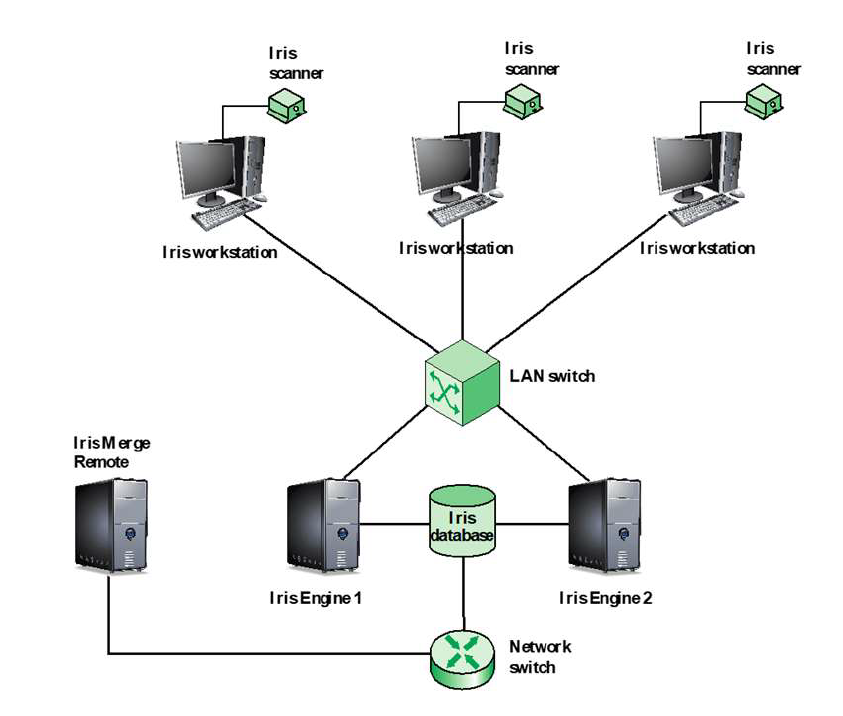
\includegraphics[scale=0.5]{../immagini/general.png}
            \end{center}
            \caption{General iris
            scan site
            architecture for
            UAE system}
        \end{figure}
        \newpage
    \subsection{Exercises}
        \subsubsection{Exercise 1}
            \subparagraph{Question: }A system requests the users to choose passwords at least 8 and at most 10 characters long and that are
            chosen within an alphabet of 40 symbols. The system combines the passwords with a 10 bits salt to
            produce a hash code for each password that is stores, along with the salt, in the password file. The hash
            is 128 bits long.
            Assume also that testing a password takes 0.1 milliseconds.
            \begin{enumerate}
                \item  An adversary that got access to the password file performs a brute force attack to crack the
                password of a specific user. How long it will take in the worst case and on average?
                \item  Assume the system has 10,000 users, and the adversary is interested in breaking the password of
                one arbitrary user (any user would be OK to get in). How long it will take on average?
                How long it would take if no salt was used?
            \end{enumerate}

            \subparagraph{Answer: }

            \begin{enumerate}
                \item Response: \[S= \text{Number of Symbols} = 40, N= \text{lengths of password} = {8,9,10}, P= \text{Number of Permutation}, C=\text{Permutation with salt}, CS=\text{Permutation of Salt} \]
                \begin{itemize}
                    \item The number of different passwords are: To calculate this number we will use Permutation with Repetition \[P=40^8+40^9+40^{10}=1.075*10^{16}\]
                    \item Each password is combined with a salt randomly chosen in  combinations: \[CS = 1024\]
                    \item Thus the number of combinations to be generated is:\[C= P*CS=1,10*10^{19}\]
                    \item In the worst case it will take: To taka worst case we consider all combination, so first we transfororm milliseconds in seconds  \[SEC = 0.1/1000 = 10^{-4}\] then we calculate number of second necessarily  \[N_{SEC} = C*SEC\] and finally transform its in year \[N_Y = N_{SEC}/SEC_Y = 3.492.794,2 years\]
                    \item On average it will take: you just need to divide by two -> \[NA_{SEC} = N_{SEC}/2\] and after \[N_Y = NA_{SEC}/SEC_y\]   
                \end{itemize}
                \item Response: 
                \begin{itemize}
                    \item The number of different passwords are: \(1.101.511.929.856.000.000\) \[C = \text{like first question}\]
                    \item Each password is combined with a salt randomly chosen in \(1024\) combinations.
                    \item On average: To calculate it,you have to multiply \[C*10.000,\text{Then to make same calculations made for first Question} and result is 17.466.263\] years to crack the password of one arbitrary user in a system with \(10.000\) users.
                    \item Thus it will take on average: \(17.466.263\) years
                    \item If no salt was used it will take on average: \(17.048\) years because we have only  permutation \[P\] as number of passwords.
                \end{itemize}
                
        \subparagraph{Question: }     
                    A system requests the users to choose passwords at least 8 and at most 10 characters long and that are
                    chosen within an alphabet of 40 symbols. The system combines the passwords with a 10 bits salt to
                    produce a hash code for each password that is stores, along with the salt, in the password file. The hash
                    is 32 bits long.
                    Assume also that testing a password takes 0.1 milliseconds.
                    An adversary that got access to the password file performs a brute force attack to crack the password of
                    a specific user. How long it will take in the worst case and on average?
        \subparagraph{Answer: }
                
                    \begin{itemize}
                        \item The number of different passwords are: Same value of previous exercise \[P\]
                        \item Each password is combined with a salt randomly chosen in \(1024\) combinations because is composed by 10 bits
                        \item The number of different hashes in which the password is encoded is: \(4.294.967.296\)
                        \item On average, the number of combinations to be generated is:
                        \item On average it will take: 
                    \end{itemize}
                
                
            \end{enumerate}

\section{Access Control}
            \subsection{Introduction}
                  \paragraph{Definition}
                    \begin{description}
                        \item[NISTIR 7298:] 
                        \begin{quote}
                            “the process of granting or denying
                            specific requests to:
                            \begin{enumerate}[label=(\arabic*)]
                                \item obtain and use information and related information processing services; and
                                \item enter specific physical facilities”
                            \end{enumerate}
                        \end{quote}
                        
                        \item[RFC 4949:] 
                        \begin{quote}
                            “a process by which use of system
                            resources is regulated according to a security
                            policy and is permitted only by authorized
                            entities (users, programs, processes, or
                            other systems) according to that policy”
                        \end{quote}
                    \end{description}
                 \paragraph{Security Requirements}
                    
                 \begin{enumerate}
                    \item Limit information system access to authorized users, processes acting on
                    behalf of authorized users, or devices (including other information systems).
                    \item Limit information system access to the types of transactions and functions
                    that authorized users are permitted to execute.
                    \item Control the flow of CUI \footnote{CUI : controlled
                    unclassified
                    information} (controlled unclassified information) in accordance
                    with approved authorizations.
                    \item Separate the duties of individuals to reduce the risk of malevolent activity
                    without collusion.
                    \item Employ the principle of least privilege, including for specific security functions
                    and privileged accounts.
                    \item Use non-privileged accounts or roles when accessing non-security functions.
                    \item Prevent non-privileged users from executing privileged functions and audit
                    the execution of such functions.
                    \item Limit unsuccessful logon attempts.
                    \item Provide privacy and security notices consistent with applicable CUI rules.
                    \item Use session lock with pattern-hiding displays to prevent access and viewing of
                    data after period of inactivity.
                    \item Terminate (automatically) a user session after a defined condition.
                    \item Monitor and control remote access sessions.
                    \item Employ cryptographic mechanisms to protect the confidentiality of remote
                    access sessions.
                    \item Route remote access via managed access control points.
                    \item Authorize remote execution of privileged commands and remote access to
                    security-relevant information.
                    \item Authorize wireless access prior to allowing such connections.
                    \item Protect wireless access using authentication and encryption.
                    \item Control connection of mobile devices.
                    \item Encrypt CUI on mobile devices.
                    \item Verify and control/limit connections to and use of external information
                    systems.
                    \item Limit use of organizational portable storage devices on external information
                    systems.
                    \item Control CUI posted or processed on publicly accessible information systems.
                \end{enumerate}
                
                \paragraph{Principles} In a broad sense, all of computer security is
                concerned with access control RFC 4949 defines computer security as:
                        \begin{quote}
                        "measures that implement and assure
                            security services in a computer system,
                            particularly those that assure access control
                            service"
                        \end{quote}
                \paragraph{Computer Security}
                We address a specific concept of access
                control, that implements a security policy, it specifies who (or what) may have access to each
                specific system resource, and the type of access that is permitted in each
                instance

                \paragraph{Other Security Functions}In addition to access control, this context involves the
                following entities and functions: 
                \begin{description}
                    \item[Authentication:] Verification that the credentials of a user or other system entity are valid.
                    \item[Authorization:] The granting of a right or permission to a system entity to access a system resource. This function determines who is trusted for a given purpose.
                    \item[Audit:] An independent review and examination:
                    \begin{itemize}
                        \item checks the adequacy of system controls,
                        \item ensures compliance with established policy and operational procedures,
                        \item detects breaches in security,
                        \item recommends any indicated changes in control, policy and procedures.
                    \end{itemize}
                \end{description}

                    \begin{figure}[h]
                        \begin{center}
                            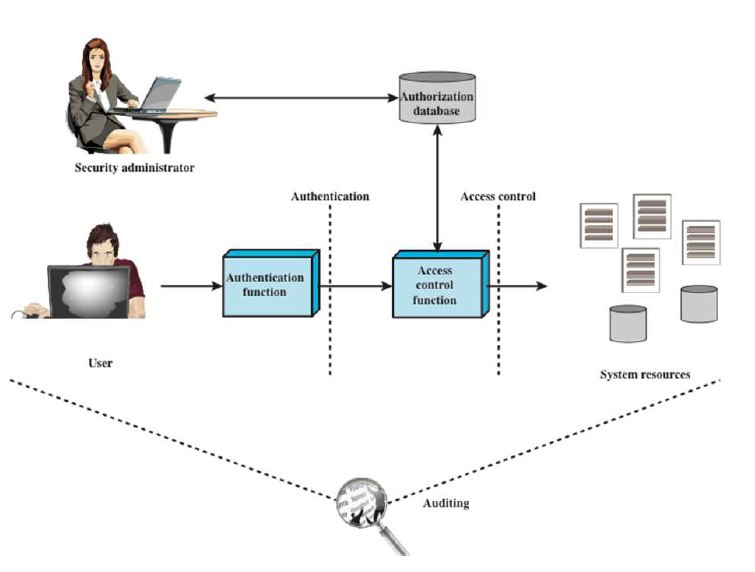
\includegraphics[scale=0.5]{../immagini/security_functions.png}
                        \end{center}
                        \caption{Security Functions}
                    \end{figure}
                
                \paragraph{Policies}
                    \begin{description}
                        \item[Discretionary access control (DAC):]
                        \begin{itemize}
                            \item Controls access based on the identity of the requestor and on access rules (authorizations) stating what requestors are (or are not) allowed to do.
                        \end{itemize}
                        \item[Mandatory access control (MAC):]
                        \begin{itemize}
                            \item Controls access based on comparing security labels with security clearances.
                        \end{itemize}
                        \item[Role-based access control (RBAC):]
                        \begin{itemize}
                            \item Controls access based on the roles that users have within the system and on rules stating what accesses are allowed to users in given roles.
                        \end{itemize}
                        \item[Attribute-based access control (ABAC):]
                        \begin{itemize}
                            \item Controls access based on attributes of the user, the resource to be accessed, and current environmental conditions.
                        \end{itemize}
                    \end{description}
                
                \paragraph{Subjects,
                objects, and
                access rights}

                \begin{description}
                    \item[Subject:] An entity
                    capable of
                    accessing
                    objects
                    \begin{itemize}
                        \item Generally, the concept of subject equates with that of process.
                        \item A user/application accesses objects by means of a process that represents it.
                        \item The process takes on the attributes of the user/application, such as access rights.
                        \item It is held accountable for its actions, an audit trail may be used to record the association of a subject with security relevant actions performed on an object by the subject.
                        \item[Three classes of subjects:]
                        \begin{description}
                            \item[Owner:] The creator of a resource (a system administrator or a project leader…).
                            \item[Group:] Membership in the group lets to exercise some access rights. A user may belong to multiple groups.
                            \item[World:] Users that are able to access the system anyway. Grants the least access rights necessary.
                        \end{description}
                    \end{itemize}
                    \item[Object:] A resource to
                    which access is
                    controlled
                    \begin{itemize}
                        \item Contains and/or receives information:
                        \begin{itemize}
                            \item records, blocks, pages, files, portions of files, directories, messages, programs etc.
                            \item may also be: bits, bytes, words, processors, ports, clocks, etc.
                        \end{itemize}
                        \item Number and types depends on:
                        \begin{itemize}
                            \item the context in which access control operates
                            \item the tradeoff between security vs complexity, processing burden, and ease of use.
                        \end{itemize}
                    \end{itemize}
                    \item[Access right:] Describes the
                    way in which a
                    subject may
                    access an object
                    \begin{itemize}
                        \item Read: view information in a system resource. Includes the ability to copy or print.
                        \item Write: add, modify, or delete data in system resource. Includes read access.
                        \item Execute: execute specified programs.
                        \item Delete: delete certain system resources, such as files or records.
                        \item Create: create new files, fields, etc.
                        \item Search: list the files in a directory or otherwise search the directory.
                    \end{itemize}
                \end{description}
            \subsection{Policies}
                \subsubsection{Discretionary access
                control (DAC)}Scheme in which an entity may be granted
                access rights that permit the entity, by its
                own volition, to enable another entity to
                access some resource. Often provided using an access matrix where One dimension consists of identified subjects
                that may attempt data access to the resources and the other dimension lists the objects that may
                be accesse, each entry in the matrix indicates the access
                rights of a particular subject for a particular
                object. 

                \begin{figure}[h]
                    \begin{center}
                        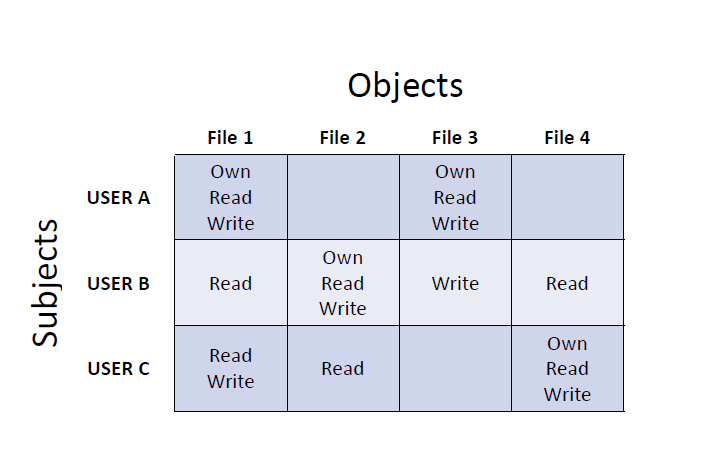
\includegraphics[scale=0.5]{../immagini/access_matrix.png}
                    \end{center}
                    \caption{Access Matrix} 
                \end{figure}

                    \paragraph{Example of access control structures}
                        \subparagraph{ACL:} Will be explanated after ...
                            \begin{figure}[h]
                                \begin{center}
                                    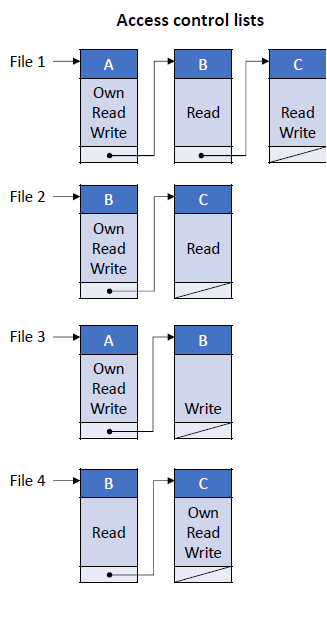
\includegraphics[scale=0.5]{../immagini/acl.png}
                                \end{center}
                                \caption{Access Control Lists}
                            \end{figure}
                            \vspace{2cm}
                        \subparagraph{Lists of capabilities (CT)}
                        Specifies authorized objects and operations for a
                        particular user. Each user has a number of tickets and may be
                        authorized to loan or give them to others. However… tickets may be dispersed around the
                        system, they present \textbf{a greater security} problem
                        than ACL.

                        \begin{itemize}
                            \item The integrity of the ticket must be protected, and guaranteed. The ticket must be unforgeable.
                            \item The OS may manage CT on behalf of users, but tickets would have to be held in a region of memory inaccessible to users.
                            \item In alternative, they may include an unforgeable token in the capability (like a cryptographic message authentication code - MAC).
                            \item The latter form of CT is appropriate in a distributed environment, when the security of its contents cannot be guaranteed.
                        \end{itemize}

                        \begin{figure}[h]
                            \begin{center}
                                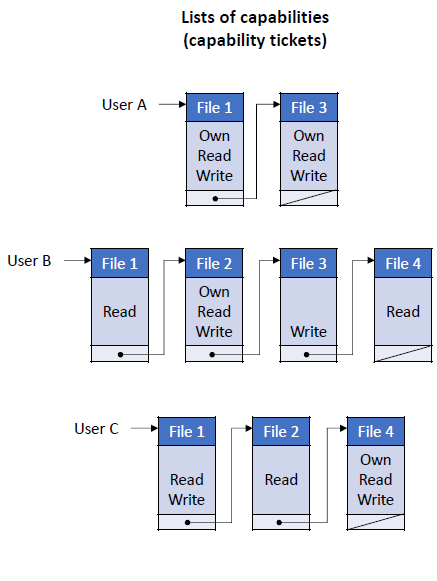
\includegraphics[scale=0.5]{../immagini/CT.png}
                            \end{center}
                            \caption{Lists of capabilities}
                        \end{figure}

                        \subparagraph{Authorization Table} Authorization table: more
                        convenient than either ACLs
                        or CT 
                        \begin{itemize}
                            \item Sorted by subject gives CT
                            \item Sorted by object gives ACL
                            \item Easy to implement in a relational database
                        \end{itemize}
                        
                        \begin{figure}[h]
                            \begin{center}
                                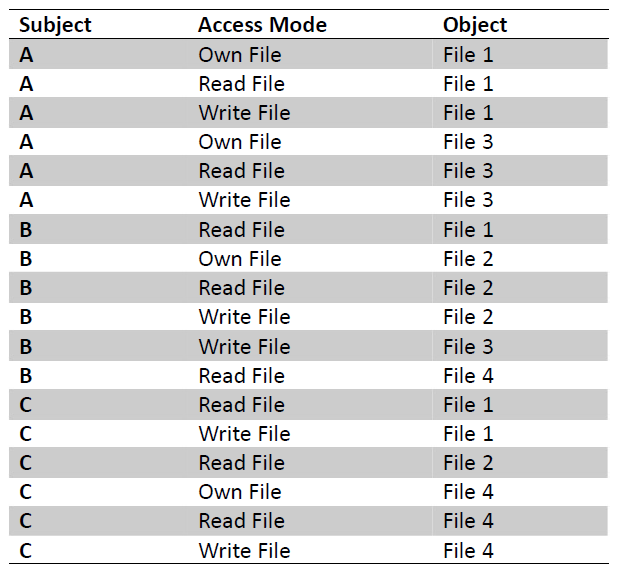
\includegraphics{../immagini/AT.png}
                            \end{center}
                            \caption{Authorization Table}
                        \end{figure}
                    \paragraph{Models} 
                            A model for DAC developed by Lampson,
                            Graham, Denning (1971/72)
                            \begin{itemize}
                                \item Protection state of a system:
                                \begin{itemize}
                                    \item the set of information, at a given time, that specifies the access rights for each subject with respect to each object
                                \end{itemize}
                                \item Requirements:
                                \begin{itemize}
                                    \item representing the protection state
                                    \item enforcing access rights
                                    \item allowing subjects to alter the protection state in certain ways
                                \end{itemize}
                            \end{itemize}

                            \subparagraph{Representing the
                            protection state}Extends the universe of objects:

                            \begin{description}
                                \item[Processes:]
                                \begin{itemize}
                                    \item Access rights include the ability to delete a process, stop (block), and wake up a process.
                                \end{itemize}
                                \item[Devices:]
                                \begin{itemize}
                                    \item Access rights include the ability to read/write the device, to control its operation (e.g., a disk seek), and to block/unblock the device for use.
                                \end{itemize}
                                \item[Memory locations or regions:]
                                \begin{itemize}
                                    \item Access rights include the ability to read/write certain regions of memory that are protected such that the default is to disallow access.
                                \end{itemize}
                                \item[Subjects:]
                                \begin{itemize}
                                    \item Access rights with respect to a subject have to do with the ability to grant or delete access rights of that subject to other objects, as explained subsequently.
                                \end{itemize}
                            \end{description}
                            
                            \begin{figure}[h]
                                \begin{center}
                                    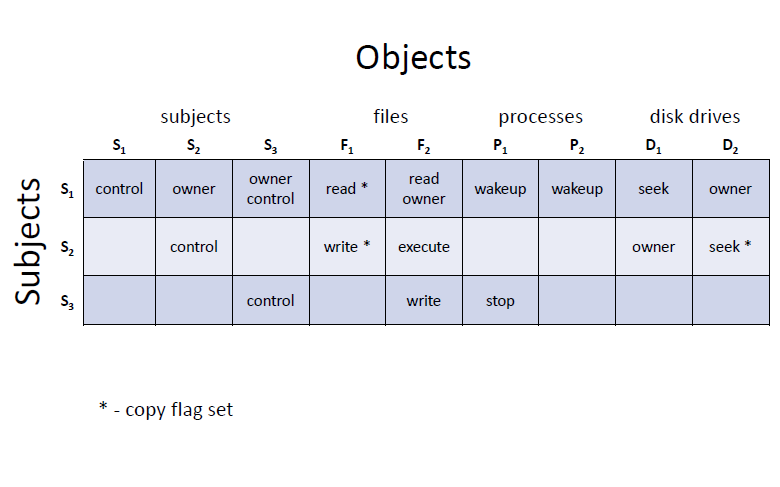
\includegraphics[scale=0.5]{../immagini/ExtendedAccessControlMatrix.png}
                                \end{center}
                                \caption{Extended Access Control Matrix}
                            \end{figure}   
                            
                            \subparagraph{Enforcing Access Rights}  This model assumes a “separate” access
                            control module for each object. An access triggers the following steps: 
                            \begin{enumerate}
                                \item A subject S0 issues a request of type $\alpha$ for object X.
                                \item The request causes the system to generate a message of the form (S0, $\alpha$, X) to the controller for X.
                                \item The controller interrogates the access matrix A to determine if $\alpha$ is in A[S0, X]:
                                \begin{itemize}
                                    \item If so, the access is allowed;
                                    \item If not, the access is denied.
                                \end{itemize}
                            \end{enumerate}
                            The model also includes rules for the
                            modification of the access matrix, need for “owner” and “control” access
                            rights to change the rights and the structure of the
                            access matrix, and  need for “copy flag” concept To give a right to another subject
                            \begin{figure}[h]
                                \begin{center}
                                    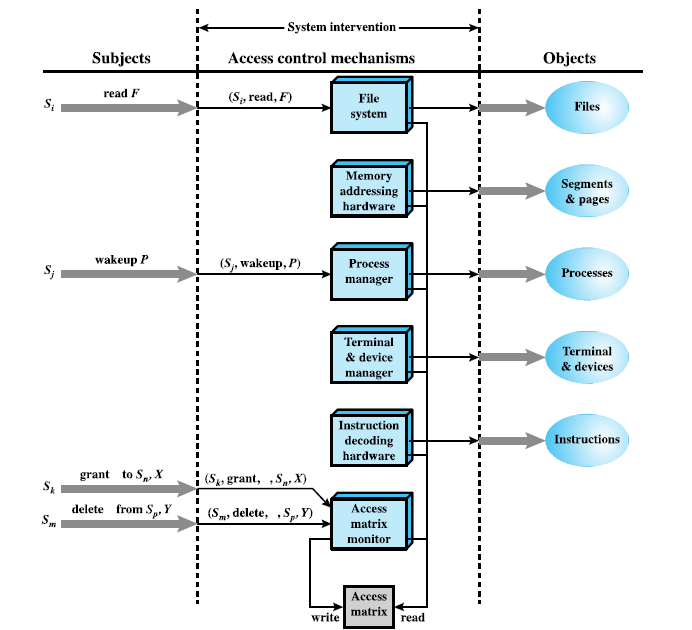
\includegraphics[scale=0.5]{../immagini/access_control_fucntion.png}
                                \end{center}
                                \caption{Organization of the access control function}
                            \end{figure}   

                            \begin{figure}[h]
                                \centering
                                \begin{subfigure}
                                    \centering
                                    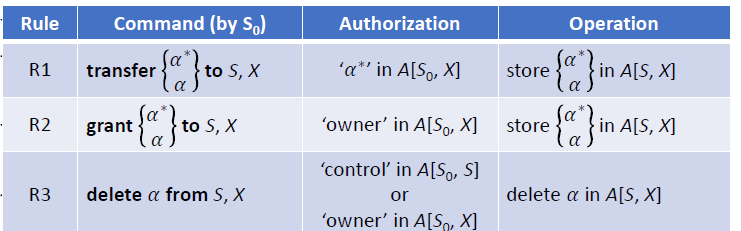
\includegraphics[scale=0.4]{../immagini/trasfering.png}
                                    \caption{Transferring, granting
                                    and deleting access
                                    rights}
                                    \label{fig:sub1}
                                \end{subfigure}
                                \hspace{1cm} % Spazio tra le due subfigures
                                \begin{subfigure}
                                    \centering
                                    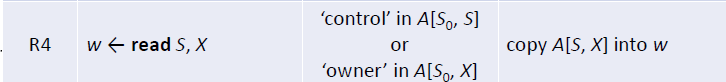
\includegraphics[scale=0.4]{../immagini/read.png}
                                    \caption{Reading the access
                                    matrix}
                                    \label{fig:sub2}
                                \end{subfigure}
                                \hspace{1cm} % Spazio tra le due subfigures
                                \begin{subfigure}
                                    \centering
                                    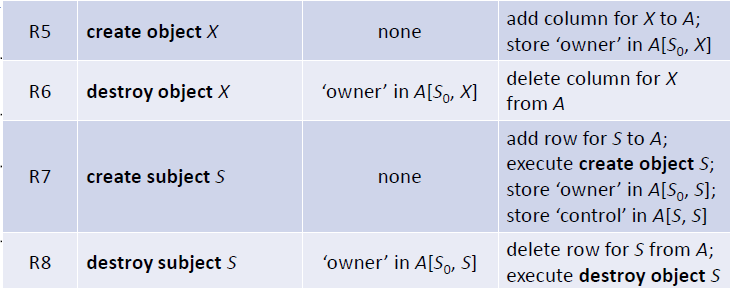
\includegraphics[scale=0.4]{../immagini/manipulating.png}
                                    \caption{Manipulating objects
                                    and subjects}
                                    \label{fig:sub3}
                                \end{subfigure}
                                \caption{Access control
                                system commands}
                                \label{fig:general}
                            \end{figure}
                        \newpage
                        \paragraph{Protection Domains} So far, a subject is a user, and a row in the access control
                        matrix represents its capabilities.It has more flexibility when associating capabilities with
                        protection domains, permit to set of objects together with access rights to those objects, in terms of the access matrix, a row defines a protection
                        domain. With flexibility a user can spawn processes with a subset of the access rights
                        of the user and association between a process and a domain can be static or
                        dynamic. In Unix, for example, in user mode certain areas of memory are protected from
                        use and certain instructions may not be executed,
                        while in kernel mode privileged instructions may be executed and
                        protected areas of memory may be accessed 
                        \newpage
                        \paragraph{Recap of  Operating Systems}
                            \begin{figure}[h]
                                \begin{center}
                                    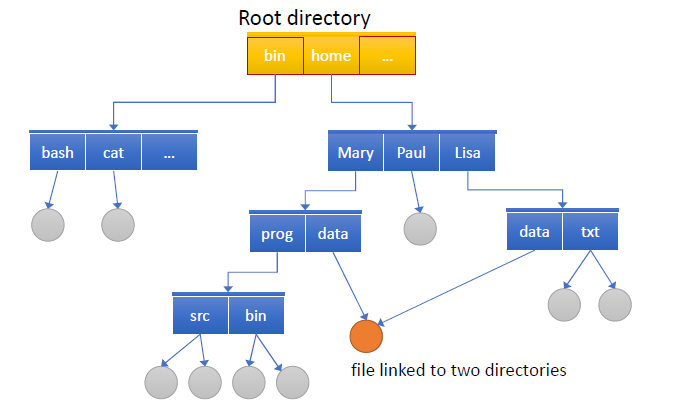
\includegraphics[scale=0.5]{../immagini/unix_file_system.png}
                                \end{center}
                                \caption{File System: tree structure}
                            \end{figure}
                            
                            \subparagraph{Directories:} In Unix each file (and directory) belongs to a
                            directory and each directory is a data structure that links
                            file names to file attributes an example of attributes are: file size, address
                            on disk, access rights, time of last
                            access, time of creation, \dots. A possible implementation is FAT file systems, where the directory is a table, it associates
                            each file name to its file descriptor. In implementation of directories in Unix the directory is a table that includes the
                            references to the file descriptors (i-nodes), which
                            are stored in a separate data structure in the disk
                            (which includes all attributes of the file)
                            \begin{description}
                                \item[/] it’s the root directory
                                \item[/bin] binary executable files. These are utilities of the system
                                \item[/boot] everything required to boot the system
                                \item[/dev] contains the device files (<<everything is a file in Unix>>\dots)
                                \begin{itemize}
                                    \item These are not regular files; accessing these files means accessing the respective system devices (drives, serial lines, etc…)
                                \end{itemize}
                                \item[/etc] contains system administration and configuration files (the file of passwords is here)
                                \item[/home] contains the users’ home directories
                                \item[/lib] contains kernel modules and the shared libraries
                                \item[/mnt] generic point under which to mount a file system or a device
                                \item[/opt] contains add-on packages not part of the default installation
                                \item[/proc] is very special in that it is also a virtual filesystem (aka process information pseudo-file system):
                                \begin{itemize}
                                    \item It doesn't contain 'real' files but runtime system information (e.g. system memory, devices mounted, hardware configuration, etc).
                                    \item It can be regarded as a control and information centre for the kernel.
                                    \item In fact, quite a lot of system utilities are simply calls to files in this directory.
                                    \item By altering files located in this directory you can even read/change kernel parameters (sysctl) while the system is running.
                                \end{itemize}
                                \item[/tmp] contains temporary files
                                \item[/usr] contains <<everything user\-related>>, for example programs for users (not system programs).
                                \begin{itemize}
                                    \item[/usr/bin] programs for the user (included games)
                                    \item[/usr/lib] libraries for user programs
                                \end{itemize}
                            \end{description}

                            \begin{figure}[h]
                                \begin{center}
                                    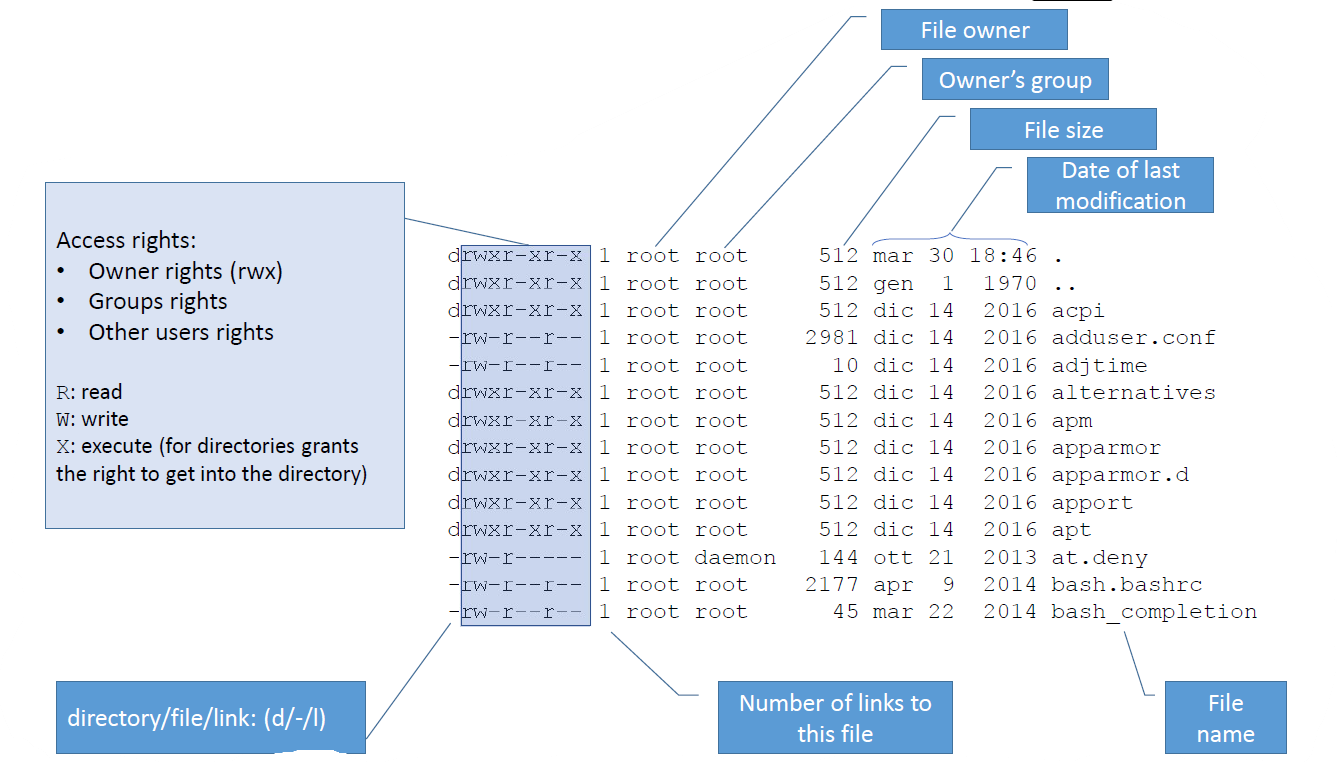
\includegraphics[scale=0.5]{../immagini/Directory_unix.png}
                                \end{center}
                                \caption{A directory in Unix}
                            \end{figure}

                            \subparagraph{Access Right}
                            Creation of users and groups (and deletion) is reserved to the root user, by means of:
                            \begin{itemize}
                                \item \texttt{useradd} / \texttt{userdel}
                                \item \texttt{groupadd} / \texttt{groupdel}
                            \end{itemize}
                            
                            \textbf{Changing Permissions to Files and Directories}\\
                            
                            To change permissions to files and directories:
                            \begin{itemize}
                                \item \texttt{chmod [a,u,g,o] [+,-] [r,w,x] file\_name} :
                                \begin{itemize}
                                    \item gives (\texttt{+}) or revokes (\texttt{-}) rights [r,w,x] to all (a), owner (u), group (g), others (o) to the file \texttt{file\_name}
                                \end{itemize}
                            \end{itemize}
                            
                            \textbf{Changing the Owner or the Group of a File}\\
                            
                            To change the owner or the group of a file:
                            \begin{itemize}
                                \item \texttt{chown new\_owner file\_name} (change owner)
                                \item \texttt{chgrp new\_group file\_name} (change group)
                            \end{itemize}

                            \subparagraph{Berkeley UNIX FFS (Fast File System)} In this kynd of file system there is a \textit{inode table} that contains all i\-nodes, that are one per file, contains metadata (like file owner, access permissions, access times \dots) and a set of pointers to data blocks.  

                            \begin{figure}
                                \begin{center}
                                    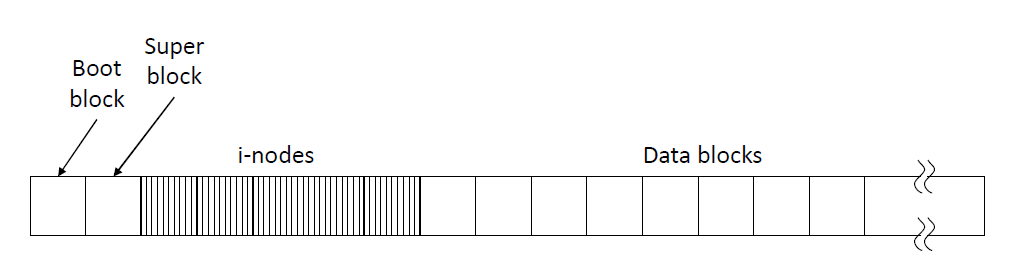
\includegraphics[scale=0.6]{../immagini/physicale_disk.png}
                                \end{center}
                                \caption{Physical disk organization in UNIX }
                            \end{figure}
                        \paragraph{Unix File access controll}

                            \subparagraph{Files}
                            UNIX files are administered using inodes (index nodes), which are control structures containing key information needed for a particular file. Several file names may be associated with a single inode. An active inode is associated with exactly one file. File attributes, permissions, and control information are stored in the inode. On the disk, there is an inode table, or inode list, that contains the inodes of all the files in the file system. When a file is opened, its inode is brought into main memory and stored in a memory resident inode table.
                            \subparagraph{Directories} 
                            May contain files and/or other directories
                            and contains file names plus pointers to associated inodes
                            
                            
                            \subparagraph{Traditional}
                            \begin{itemize}
                                \item A user:
                                \begin{itemize}
                                    \item Unique user identification number (user ID)
                                    \item Member of a primary group identified by a group ID
                                    \item May also belong to several other groups
                                \end{itemize}
                                \item A file (an object):
                                \begin{itemize}
                                    \item Has an owner
                                    \item 12 protection bits
                                    \item Specify read, write, and execute permission for the owner of the file, members of the group and all other users
                                    \item The owner ID, group ID, and protection bits are part of the file’s inode
                                \end{itemize}
                                \item A hierarchy:
                                \begin{itemize}
                                    \item owner – group – all others
                                \end{itemize}
                                \item Concerning directories:
                                \begin{itemize}
                                    \item Read grants the list capability
                                    \item Write grants the create / rename / delete files capability
                                    \item Execute grants the ability to descend into subdirectories
                                \end{itemize}
                                \item “Set user ID” (SetUID) and “Set group ID” (SetGID)
                                \begin{itemize}
                                    \item System temporarily uses rights of the file owner/group in addition to the real user’s rights when making access control decisions
                                    \item Enables privileged programs to access files/resources not generally accessible
                                \end{itemize}
                                \item Sticky bit
                                \begin{itemize}
                                    \item When applied to a directory it specifies that only the owner of any file in the directory can rename, move, or delete that file
                                \end{itemize}
                                \item Superuser
                                \begin{itemize}
                                    \item A specific User ID
                                    \item Is exempt from usual access control restrictions
                                    \item Has system-wide access
                                \end{itemize}

                            \end{itemize}
                            \begin{figure}[h]
                                \begin{center}
                                    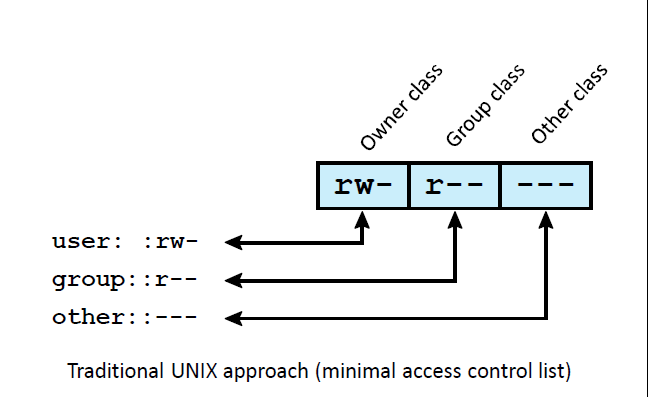
\includegraphics[scale=0.6]{../immagini/minimal_acl.png}
                                \end{center}
                                \caption{Traditiona ACL}
                            \end{figure}
                            
                            \subparagraph{Modern}
                            Many moderna Unix systems support ACLs as OpenBSD,Linux,Solaris, FreeBSD. In the last The administrator can assign a list of UNIX user IDs and groups by means of the Setfacl command. Any number of users and groups can be associated with a file, each with read, write, and execute protection bits. A file does not need to have an ACL; it includes an additional protection bit that indicates whether the file has an extended ACL.
                            
                                \textbf{Steps for process request:}\\
                                \begin{enumerate}
                                    \item Select the ACL that closely matches the requesting process
                                    \begin{itemize}
                                        \item In this order: owner, named users, groups, others
                                    \end{itemize}
                                    \item Check if the matching entry contains sufficient permissions
                                    \begin{itemize}
                                        \item A process can be in more than one group, just one is sufficient
                                    \end{itemize}
                                \end{enumerate}
                                \begin{figure}[h]
                                    \begin{center}
                                        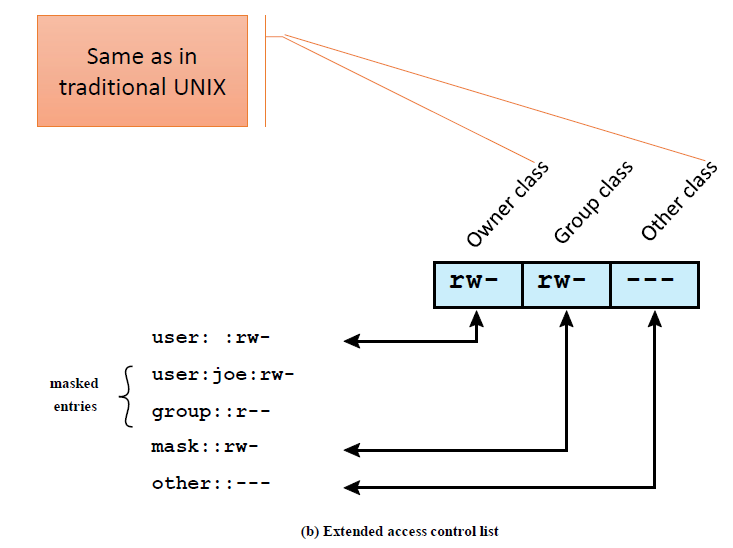
\includegraphics[scale=0.6]{../immagini/eacl.png}
                                    \end{center}
                                    \caption{Traditiona ACL}
                                \end{figure}

                        \paragraph{Exercises}
                                \begin{enumerate}
                                    \item For the DAC model, an alternative representation of the protection state is a directed graph.
                                    \item Each subject and each object in the protection state is represented by a node (a single node is used for an entity that is both subject and object).
                                    \item A directed line from a subject to an object indicates an access right, and the label on the link defines the access right.
                                \end{enumerate}
                                \subparagraph{Question}
                                Draw a directed graph that corresponds to
                                the access matrix of the figure

                                \begin{figure}[h]
                                    \begin{center}
                                        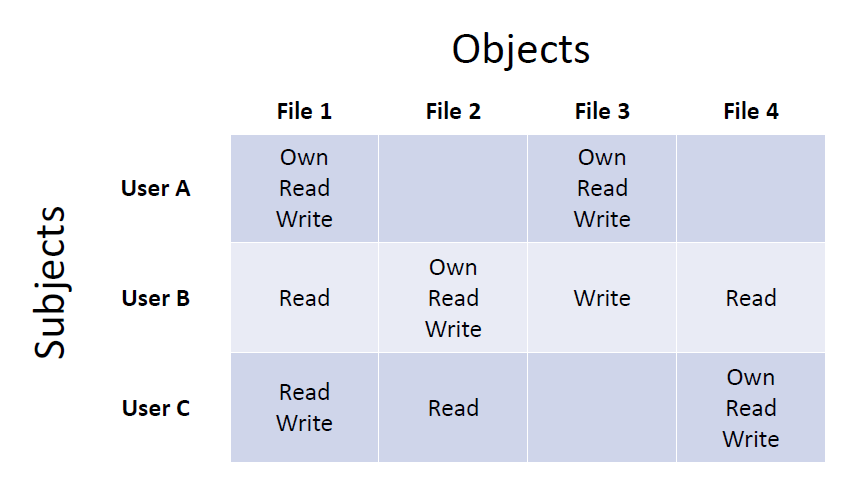
\includegraphics[scale=0.6]{../immagini/exacla.png}
                                    \end{center}
                                    
                                \end{figure}

                                \subparagraph{Answer}
                                    


                                    \tikzset{every picture/.style={line width=0.75pt}} %set default line width to 0.75pt        

                                    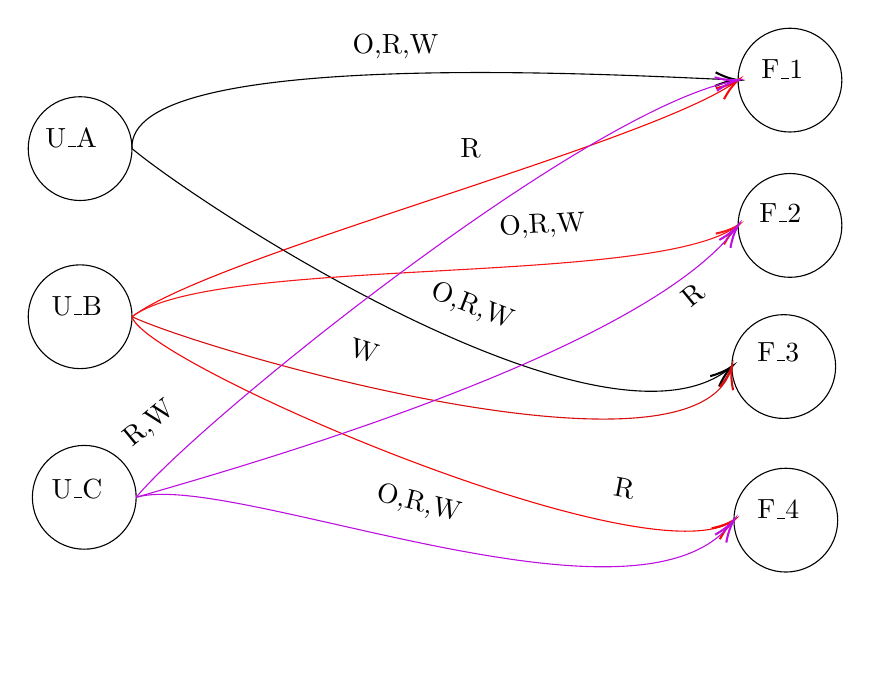
\begin{tikzpicture}[x=0.75pt,y=0.75pt,yscale=-1,xscale=1]
                                    %uncomment if require: \path (0,300); %set diagram left start at 0, and has height of 300

                                    %Shape: Circle [id:dp04479067309381324] 
                                    \draw   (126,71) .. controls (126,57.19) and (137.19,46) .. (151,46) .. controls (164.81,46) and (176,57.19) .. (176,71) .. controls (176,84.81) and (164.81,96) .. (151,96) .. controls (137.19,96) and (126,84.81) .. (126,71) -- cycle ;
                                    %Shape: Circle [id:dp6101273899231423] 
                                    \draw   (126,152) .. controls (126,138.19) and (137.19,127) .. (151,127) .. controls (164.81,127) and (176,138.19) .. (176,152) .. controls (176,165.81) and (164.81,177) .. (151,177) .. controls (137.19,177) and (126,165.81) .. (126,152) -- cycle ;
                                    %Shape: Circle [id:dp34424468948309817] 
                                    \draw   (128,239) .. controls (128,225.19) and (139.19,214) .. (153,214) .. controls (166.81,214) and (178,225.19) .. (178,239) .. controls (178,252.81) and (166.81,264) .. (153,264) .. controls (139.19,264) and (128,252.81) .. (128,239) -- cycle ;
                                    %Shape: Circle [id:dp9243554390035913] 
                                    \draw   (468,38) .. controls (468,24.19) and (479.19,13) .. (493,13) .. controls (506.81,13) and (518,24.19) .. (518,38) .. controls (518,51.81) and (506.81,63) .. (493,63) .. controls (479.19,63) and (468,51.81) .. (468,38) -- cycle ;
                                    %Shape: Circle [id:dp24525392857995354] 
                                    \draw   (468,108) .. controls (468,94.19) and (479.19,83) .. (493,83) .. controls (506.81,83) and (518,94.19) .. (518,108) .. controls (518,121.81) and (506.81,133) .. (493,133) .. controls (479.19,133) and (468,121.81) .. (468,108) -- cycle ;
                                    %Shape: Circle [id:dp0958263933335477] 
                                    \draw   (465,176) .. controls (465,162.19) and (476.19,151) .. (490,151) .. controls (503.81,151) and (515,162.19) .. (515,176) .. controls (515,189.81) and (503.81,201) .. (490,201) .. controls (476.19,201) and (465,189.81) .. (465,176) -- cycle ;
                                    %Shape: Circle [id:dp2586047953927775] 
                                    \draw   (466,250) .. controls (466,236.19) and (477.19,225) .. (491,225) .. controls (504.81,225) and (516,236.19) .. (516,250) .. controls (516,263.81) and (504.81,275) .. (491,275) .. controls (477.19,275) and (466,263.81) .. (466,250) -- cycle ;
                                    %Curve Lines [id:da12298718201049708] 
                                    \draw    (176,71) .. controls (173.03,22.09) and (407.24,35.33) .. (466.27,37.92) ;
                                    \draw [shift={(468,38)}, rotate = 182.45] [color={rgb, 255:red, 0; green, 0; blue, 0 }  ][line width=0.75]    (10.93,-3.29) .. controls (6.95,-1.4) and (3.31,-0.3) .. (0,0) .. controls (3.31,0.3) and (6.95,1.4) .. (10.93,3.29)   ;
                                    %Curve Lines [id:da16218744628671256] 
                                    \draw    (176,71) .. controls (212.82,101.45) and (404.07,225.35) .. (464.1,176.75) ;
                                    \draw [shift={(465,176)}, rotate = 139.38] [color={rgb, 255:red, 0; green, 0; blue, 0 }  ][line width=0.75]    (10.93,-3.29) .. controls (6.95,-1.4) and (3.31,-0.3) .. (0,0) .. controls (3.31,0.3) and (6.95,1.4) .. (10.93,3.29)   ;
                                    %Curve Lines [id:da7408260147522898] 
                                    \draw [color={rgb, 255:red, 244; green, 7; blue, 7 }  ,draw opacity=1 ]   (176,152) .. controls (215.6,122.3) and (423.78,69.08) .. (466.75,38.91) ;
                                    \draw [shift={(468,38)}, rotate = 143.13] [color={rgb, 255:red, 244; green, 7; blue, 7 }  ,draw opacity=1 ][line width=0.75]    (10.93,-3.29) .. controls (6.95,-1.4) and (3.31,-0.3) .. (0,0) .. controls (3.31,0.3) and (6.95,1.4) .. (10.93,3.29)   ;
                                    %Curve Lines [id:da08990746443878006] 
                                    \draw [color={rgb, 255:red, 246; green, 25; blue, 25 }  ,draw opacity=1 ]   (176,152) .. controls (215.6,122.3) and (423.78,137.68) .. (466.75,108.89) ;
                                    \draw [shift={(468,108)}, rotate = 143.13] [color={rgb, 255:red, 246; green, 25; blue, 25 }  ,draw opacity=1 ][line width=0.75]    (10.93,-3.29) .. controls (6.95,-1.4) and (3.31,-0.3) .. (0,0) .. controls (3.31,0.3) and (6.95,1.4) .. (10.93,3.29)   ;
                                    %Curve Lines [id:da8941043263144446] 
                                    \draw [color={rgb, 255:red, 215; green, 15; blue, 15 }  ,draw opacity=1 ]   (176,152) .. controls (213.62,169.42) and (445.3,236.25) .. (464.48,177.81) ;
                                    \draw [shift={(465,176)}, rotate = 103.69] [color={rgb, 255:red, 215; green, 15; blue, 15 }  ,draw opacity=1 ][line width=0.75]    (10.93,-3.29) .. controls (6.95,-1.4) and (3.31,-0.3) .. (0,0) .. controls (3.31,0.3) and (6.95,1.4) .. (10.93,3.29)   ;
                                    %Curve Lines [id:da578818340480149] 
                                    \draw [color={rgb, 255:red, 244; green, 7; blue, 7 }  ,draw opacity=1 ]   (176,152) .. controls (181.94,174.37) and (421.14,277.9) .. (464.74,250.86) ;
                                    \draw [shift={(466,250)}, rotate = 143.13] [color={rgb, 255:red, 244; green, 7; blue, 7 }  ,draw opacity=1 ][line width=0.75]    (10.93,-3.29) .. controls (6.95,-1.4) and (3.31,-0.3) .. (0,0) .. controls (3.31,0.3) and (6.95,1.4) .. (10.93,3.29)   ;
                                    %Curve Lines [id:da5363560468296524] 
                                    \draw [color={rgb, 255:red, 189; green, 16; blue, 224 }  ,draw opacity=1 ]   (178,239) .. controls (208.85,201.79) and (394.13,52.11) .. (466.91,38.2) ;
                                    \draw [shift={(468,38)}, rotate = 170.07] [color={rgb, 255:red, 189; green, 16; blue, 224 }  ,draw opacity=1 ][line width=0.75]    (10.93,-3.29) .. controls (6.95,-1.4) and (3.31,-0.3) .. (0,0) .. controls (3.31,0.3) and (6.95,1.4) .. (10.93,3.29)   ;
                                    %Curve Lines [id:da9611203442875336] 
                                    \draw [color={rgb, 255:red, 189; green, 16; blue, 224 }  ,draw opacity=1 ]   (178,239) .. controls (223.77,225.67) and (422,170.16) .. (467.33,108.92) ;
                                    \draw [shift={(468,108)}, rotate = 125.54] [color={rgb, 255:red, 189; green, 16; blue, 224 }  ,draw opacity=1 ][line width=0.75]    (10.93,-3.29) .. controls (6.95,-1.4) and (3.31,-0.3) .. (0,0) .. controls (3.31,0.3) and (6.95,1.4) .. (10.93,3.29)   ;
                                    %Curve Lines [id:da0743125835155738] 
                                    \draw [color={rgb, 255:red, 189; green, 16; blue, 224 }  ,draw opacity=1 ]   (178,239) .. controls (223.77,225.67) and (420.02,310.74) .. (465.33,250.91) ;
                                    \draw [shift={(466,250)}, rotate = 125.54] [color={rgb, 255:red, 189; green, 16; blue, 224 }  ,draw opacity=1 ][line width=0.75]    (10.93,-3.29) .. controls (6.95,-1.4) and (3.31,-0.3) .. (0,0) .. controls (3.31,0.3) and (6.95,1.4) .. (10.93,3.29)   ;

                                    % Text Node
                                    \draw (133,60) node [anchor=north west][inner sep=0.75pt]   [align=left] {U\_A};
                                    % Text Node
                                    \draw (136,141) node [anchor=north west][inner sep=0.75pt]   [align=left] {U\_B};
                                    % Text Node
                                    \draw (136,229) node [anchor=north west][inner sep=0.75pt]   [align=left] {U\_C};
                                    % Text Node
                                    \draw (478,27) node [anchor=north west][inner sep=0.75pt]   [align=left] {F\_1};
                                    % Text Node
                                    \draw (477,96) node [anchor=north west][inner sep=0.75pt]   [align=left] {F\_2};
                                    % Text Node
                                    \draw (476,163) node [anchor=north west][inner sep=0.75pt]   [align=left] {F\_3};
                                    % Text Node
                                    \draw (476,239) node [anchor=north west][inner sep=0.75pt]   [align=left] {F\_4};
                                    % Text Node
                                    \draw (281,15) node [anchor=north west][inner sep=0.75pt]   [align=left] {O,R,W};
                                    % Text Node
                                    \draw (333,65) node [anchor=north west][inner sep=0.75pt]   [align=left] {R};
                                    % Text Node
                                    \draw (321.82,132.62) node [anchor=north west][inner sep=0.75pt]  [rotate=-21.02] [align=left] {O,R,W};
                                    % Text Node
                                    \draw (351.41,102.4) node [anchor=north west][inner sep=0.75pt]  [rotate=-356.89] [align=left] {O,R,W};
                                    % Text Node
                                    \draw (281.75,160.6) node [anchor=north west][inner sep=0.75pt]  [rotate=-16.78] [align=left] {W};
                                    % Text Node
                                    \draw (408.34,227.68) node [anchor=north west][inner sep=0.75pt]  [rotate=-11] [align=left] {R};
                                    % Text Node
                                    \draw (168.5,207.82) node [anchor=north west][inner sep=0.75pt]  [rotate=-320.56] [align=left] {R,W};
                                    % Text Node
                                    \draw (437.52,140.69) node [anchor=north west][inner sep=0.75pt]  [rotate=-320.62] [align=left] {R};
                                    % Text Node
                                    \draw (294.39,230.36) node [anchor=north west][inner sep=0.75pt]  [rotate=-13.5] [align=left] {O,R,W};
                                    \end{tikzpicture}

                        \subparagraph{Question}
                        Draw a directed graph that corresponds to
                        the access matrix of the table:
                        \begin{figure}[h]
                            \begin{center}
                                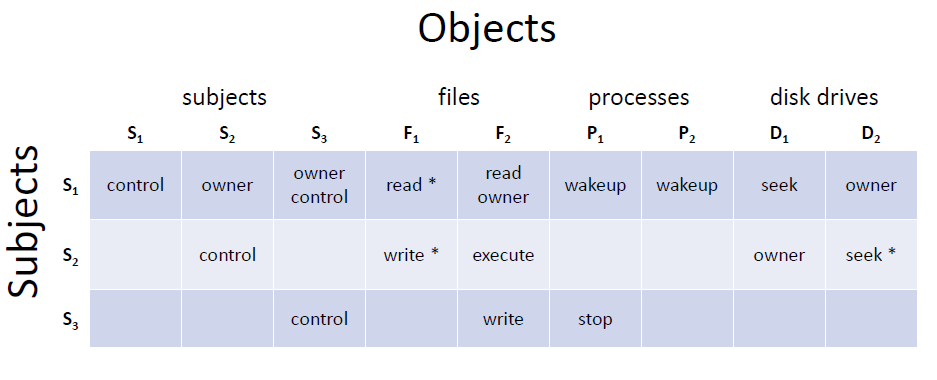
\includegraphics[scale=0.6]{../immagini/exaclb.png}
                            \end{center}
                            
                        \end{figure}
                        \subparagraph{Answer}
                            


                                            \tikzset{every picture/.style={line width=0.75pt}} %set default line width to 0.75pt        

                                            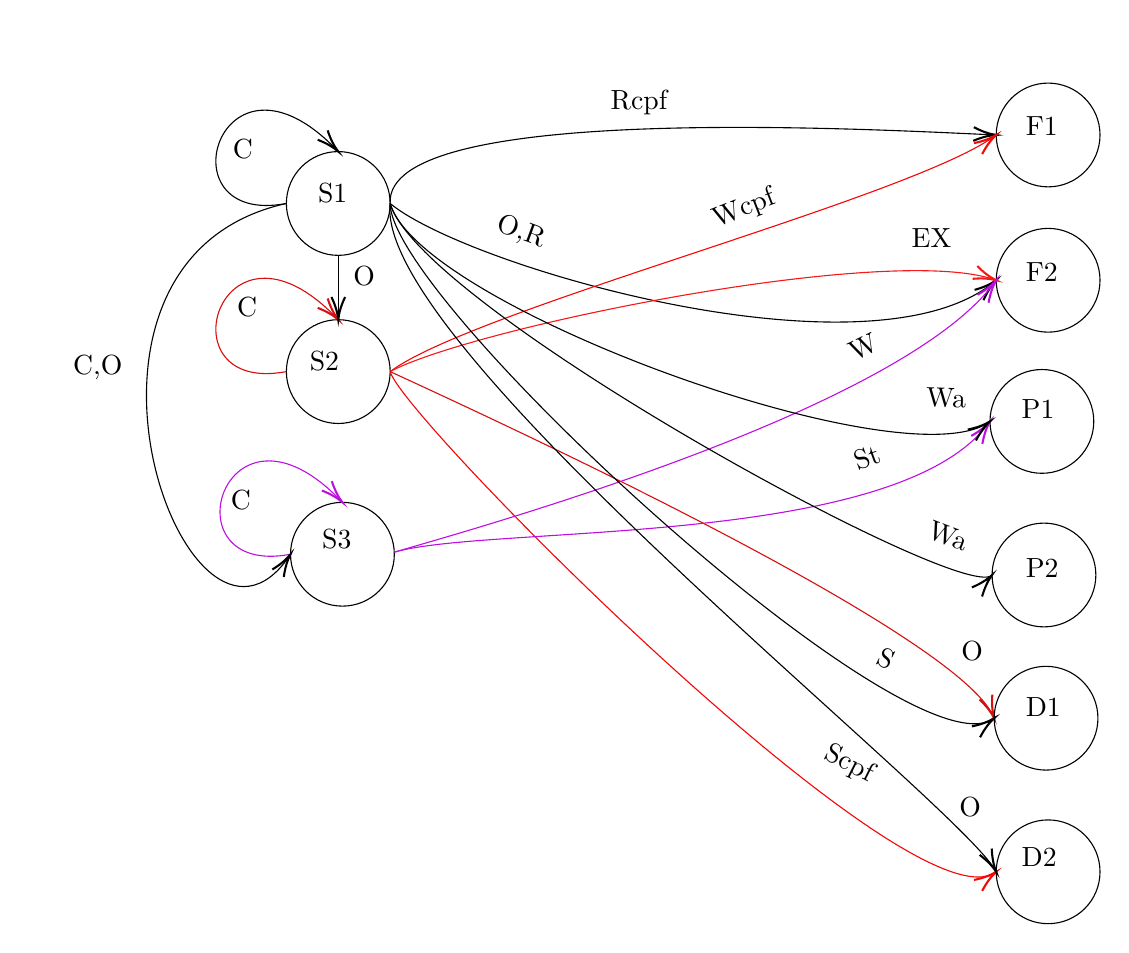
\begin{tikzpicture}[x=0.75pt,y=0.75pt,yscale=-1,xscale=1]
                                            %uncomment if require: \path (0,454); %set diagram left start at 0, and has height of 454

                                            %Shape: Circle [id:dp04479067309381324] 
                                            \draw   (126,71) .. controls (126,57.19) and (137.19,46) .. (151,46) .. controls (164.81,46) and (176,57.19) .. (176,71) .. controls (176,84.81) and (164.81,96) .. (151,96) .. controls (137.19,96) and (126,84.81) .. (126,71) -- cycle ;
                                            %Shape: Circle [id:dp6101273899231423] 
                                            \draw   (126,152) .. controls (126,138.19) and (137.19,127) .. (151,127) .. controls (164.81,127) and (176,138.19) .. (176,152) .. controls (176,165.81) and (164.81,177) .. (151,177) .. controls (137.19,177) and (126,165.81) .. (126,152) -- cycle ;
                                            %Shape: Circle [id:dp34424468948309817] 
                                            \draw   (128,240) .. controls (128,226.19) and (139.19,215) .. (153,215) .. controls (166.81,215) and (178,226.19) .. (178,240) .. controls (178,253.81) and (166.81,265) .. (153,265) .. controls (139.19,265) and (128,253.81) .. (128,240) -- cycle ;
                                            %Shape: Circle [id:dp9243554390035913] 
                                            \draw   (468,38) .. controls (468,24.19) and (479.19,13) .. (493,13) .. controls (506.81,13) and (518,24.19) .. (518,38) .. controls (518,51.81) and (506.81,63) .. (493,63) .. controls (479.19,63) and (468,51.81) .. (468,38) -- cycle ;
                                            %Shape: Circle [id:dp24525392857995354] 
                                            \draw   (468,108) .. controls (468,94.19) and (479.19,83) .. (493,83) .. controls (506.81,83) and (518,94.19) .. (518,108) .. controls (518,121.81) and (506.81,133) .. (493,133) .. controls (479.19,133) and (468,121.81) .. (468,108) -- cycle ;
                                            %Shape: Circle [id:dp0958263933335477] 
                                            \draw   (465,176) .. controls (465,162.19) and (476.19,151) .. (490,151) .. controls (503.81,151) and (515,162.19) .. (515,176) .. controls (515,189.81) and (503.81,201) .. (490,201) .. controls (476.19,201) and (465,189.81) .. (465,176) -- cycle ;
                                            %Shape: Circle [id:dp2586047953927775] 
                                            \draw   (466,250) .. controls (466,236.19) and (477.19,225) .. (491,225) .. controls (504.81,225) and (516,236.19) .. (516,250) .. controls (516,263.81) and (504.81,275) .. (491,275) .. controls (477.19,275) and (466,263.81) .. (466,250) -- cycle ;
                                            %Curve Lines [id:da12298718201049708] 
                                            \draw    (176,71) .. controls (173.03,22.09) and (407.24,35.33) .. (466.27,37.92) ;
                                            \draw [shift={(468,38)}, rotate = 182.45] [color={rgb, 255:red, 0; green, 0; blue, 0 }  ][line width=0.75]    (10.93,-3.29) .. controls (6.95,-1.4) and (3.31,-0.3) .. (0,0) .. controls (3.31,0.3) and (6.95,1.4) .. (10.93,3.29)   ;
                                            %Curve Lines [id:da16218744628671256] 
                                            \draw    (176,71) .. controls (212.82,101.45) and (407.04,158.03) .. (467.1,108.75) ;
                                            \draw [shift={(468,108)}, rotate = 139.38] [color={rgb, 255:red, 0; green, 0; blue, 0 }  ][line width=0.75]    (10.93,-3.29) .. controls (6.95,-1.4) and (3.31,-0.3) .. (0,0) .. controls (3.31,0.3) and (6.95,1.4) .. (10.93,3.29)   ;
                                            %Curve Lines [id:da7408260147522898] 
                                            \draw [color={rgb, 255:red, 244; green, 7; blue, 7 }  ,draw opacity=1 ]   (176,152) .. controls (215.6,122.3) and (423.78,69.08) .. (466.75,38.91) ;
                                            \draw [shift={(468,38)}, rotate = 143.13] [color={rgb, 255:red, 244; green, 7; blue, 7 }  ,draw opacity=1 ][line width=0.75]    (10.93,-3.29) .. controls (6.95,-1.4) and (3.31,-0.3) .. (0,0) .. controls (3.31,0.3) and (6.95,1.4) .. (10.93,3.29)   ;
                                            %Curve Lines [id:da08990746443878006] 
                                            \draw [color={rgb, 255:red, 246; green, 25; blue, 25 }  ,draw opacity=1 ]   (176,152) .. controls (204.69,136.65) and (316.75,111.21) .. (396.26,104.85) .. controls (426.34,102.44) and (451.76,102.77) .. (466.25,107.4) ;
                                            \draw [shift={(468,108)}, rotate = 200.2] [color={rgb, 255:red, 246; green, 25; blue, 25 }  ,draw opacity=1 ][line width=0.75]    (10.93,-3.29) .. controls (6.95,-1.4) and (3.31,-0.3) .. (0,0) .. controls (3.31,0.3) and (6.95,1.4) .. (10.93,3.29)   ;
                                            %Curve Lines [id:da8941043263144446] 
                                            \draw [color={rgb, 255:red, 215; green, 15; blue, 15 }  ,draw opacity=1 ]   (176,152) .. controls (213.62,169.42) and (446.28,275.45) .. (466.45,317.74) ;
                                            \draw [shift={(467,319)}, rotate = 248.87] [color={rgb, 255:red, 215; green, 15; blue, 15 }  ,draw opacity=1 ][line width=0.75]    (10.93,-3.29) .. controls (6.95,-1.4) and (3.31,-0.3) .. (0,0) .. controls (3.31,0.3) and (6.95,1.4) .. (10.93,3.29)   ;
                                            %Curve Lines [id:da578818340480149] 
                                            \draw [color={rgb, 255:red, 244; green, 7; blue, 7 }  ,draw opacity=1 ]   (176,152) .. controls (181.94,174.37) and (423.1,418.05) .. (466.74,393.82) ;
                                            \draw [shift={(468,393)}, rotate = 143.13] [color={rgb, 255:red, 244; green, 7; blue, 7 }  ,draw opacity=1 ][line width=0.75]    (10.93,-3.29) .. controls (6.95,-1.4) and (3.31,-0.3) .. (0,0) .. controls (3.31,0.3) and (6.95,1.4) .. (10.93,3.29)   ;
                                            %Curve Lines [id:da9611203442875336] 
                                            \draw [color={rgb, 255:red, 189; green, 16; blue, 224 }  ,draw opacity=1 ]   (178,239) .. controls (223.77,225.67) and (422,170.16) .. (467.33,108.92) ;
                                            \draw [shift={(468,108)}, rotate = 125.54] [color={rgb, 255:red, 189; green, 16; blue, 224 }  ,draw opacity=1 ][line width=0.75]    (10.93,-3.29) .. controls (6.95,-1.4) and (3.31,-0.3) .. (0,0) .. controls (3.31,0.3) and (6.95,1.4) .. (10.93,3.29)   ;
                                            %Curve Lines [id:da0743125835155738] 
                                            \draw [color={rgb, 255:red, 189; green, 16; blue, 224 }  ,draw opacity=1 ]   (178,239) .. controls (223.77,225.67) and (419.03,237.48) .. (464.33,176.92) ;
                                            \draw [shift={(465,176)}, rotate = 125.54] [color={rgb, 255:red, 189; green, 16; blue, 224 }  ,draw opacity=1 ][line width=0.75]    (10.93,-3.29) .. controls (6.95,-1.4) and (3.31,-0.3) .. (0,0) .. controls (3.31,0.3) and (6.95,1.4) .. (10.93,3.29)   ;
                                            %Shape: Circle [id:dp32805782322149213] 
                                            \draw   (467,319) .. controls (467,305.19) and (478.19,294) .. (492,294) .. controls (505.81,294) and (517,305.19) .. (517,319) .. controls (517,332.81) and (505.81,344) .. (492,344) .. controls (478.19,344) and (467,332.81) .. (467,319) -- cycle ;
                                            %Shape: Circle [id:dp4521304677570057] 
                                            \draw   (468,393) .. controls (468,379.19) and (479.19,368) .. (493,368) .. controls (506.81,368) and (518,379.19) .. (518,393) .. controls (518,406.81) and (506.81,418) .. (493,418) .. controls (479.19,418) and (468,406.81) .. (468,393) -- cycle ;
                                            %Curve Lines [id:da1654541029491967] 
                                            \draw    (126,71) .. controls (65.3,82.54) and (93.71,-13.43) .. (150.15,45.11) ;
                                            \draw [shift={(151,46)}, rotate = 226.66] [color={rgb, 255:red, 0; green, 0; blue, 0 }  ][line width=0.75]    (10.93,-3.29) .. controls (6.95,-1.4) and (3.31,-0.3) .. (0,0) .. controls (3.31,0.3) and (6.95,1.4) .. (10.93,3.29)   ;
                                            %Curve Lines [id:da19446495687177934] 
                                            \draw [color={rgb, 255:red, 215; green, 15; blue, 15 }  ,draw opacity=1 ]   (126,152) .. controls (65.3,163.54) and (93.71,67.57) .. (150.15,126.11) ;
                                            \draw [shift={(151,127)}, rotate = 226.66] [color={rgb, 255:red, 215; green, 15; blue, 15 }  ,draw opacity=1 ][line width=0.75]    (10.93,-3.29) .. controls (6.95,-1.4) and (3.31,-0.3) .. (0,0) .. controls (3.31,0.3) and (6.95,1.4) .. (10.93,3.29)   ;
                                            %Curve Lines [id:da616097024929599] 
                                            \draw [color={rgb, 255:red, 189; green, 16; blue, 224 }  ,draw opacity=1 ]   (128,240) .. controls (67.3,251.54) and (95.71,155.57) .. (152.15,214.11) ;
                                            \draw [shift={(153,215)}, rotate = 226.66] [color={rgb, 255:red, 189; green, 16; blue, 224 }  ,draw opacity=1 ][line width=0.75]    (10.93,-3.29) .. controls (6.95,-1.4) and (3.31,-0.3) .. (0,0) .. controls (3.31,0.3) and (6.95,1.4) .. (10.93,3.29)   ;
                                            %Straight Lines [id:da8939300728664765] 
                                            \draw    (151,96) -- (151,125) ;
                                            \draw [shift={(151,127)}, rotate = 270] [color={rgb, 255:red, 0; green, 0; blue, 0 }  ][line width=0.75]    (10.93,-3.29) .. controls (6.95,-1.4) and (3.31,-0.3) .. (0,0) .. controls (3.31,0.3) and (6.95,1.4) .. (10.93,3.29)   ;
                                            %Curve Lines [id:da06285582164839654] 
                                            \draw    (126,71) .. controls (1.62,98.46) and (78.23,312.44) .. (127.26,241.1) ;
                                            \draw [shift={(128,240)}, rotate = 123.3] [color={rgb, 255:red, 0; green, 0; blue, 0 }  ][line width=0.75]    (10.93,-3.29) .. controls (6.95,-1.4) and (3.31,-0.3) .. (0,0) .. controls (3.31,0.3) and (6.95,1.4) .. (10.93,3.29)   ;
                                            %Curve Lines [id:da3350118800335362] 
                                            \draw    (176,71) .. controls (189.86,120.1) and (420.32,204.3) .. (463.74,176.87) ;
                                            \draw [shift={(465,176)}, rotate = 143.13] [color={rgb, 255:red, 0; green, 0; blue, 0 }  ][line width=0.75]    (10.93,-3.29) .. controls (6.95,-1.4) and (3.31,-0.3) .. (0,0) .. controls (3.31,0.3) and (6.95,1.4) .. (10.93,3.29)   ;
                                            %Curve Lines [id:da30582359908076584] 
                                            \draw    (176,71) .. controls (189.65,119.36) and (440.01,257.46) .. (464.56,250.8) ;
                                            \draw [shift={(466,250)}, rotate = 131.68] [color={rgb, 255:red, 0; green, 0; blue, 0 }  ][line width=0.75]    (10.93,-3.29) .. controls (6.95,-1.4) and (3.31,-0.3) .. (0,0) .. controls (3.31,0.3) and (6.95,1.4) .. (10.93,3.29)   ;
                                            %Curve Lines [id:da874215087152979] 
                                            \draw    (176,71) .. controls (176,117.13) and (422.01,344.39) .. (465.74,319.82) ;
                                            \draw [shift={(467,319)}, rotate = 143.13] [color={rgb, 255:red, 0; green, 0; blue, 0 }  ][line width=0.75]    (10.93,-3.29) .. controls (6.95,-1.4) and (3.31,-0.3) .. (0,0) .. controls (3.31,0.3) and (6.95,1.4) .. (10.93,3.29)   ;
                                            %Curve Lines [id:da017874621786993394] 
                                            \draw    (176,71) .. controls (168.12,138.57) and (442.58,354) .. (467.06,391.42) ;
                                            \draw [shift={(468,393)}, rotate = 242.31] [color={rgb, 255:red, 0; green, 0; blue, 0 }  ][line width=0.75]    (10.93,-3.29) .. controls (6.95,-1.4) and (3.31,-0.3) .. (0,0) .. controls (3.31,0.3) and (6.95,1.4) .. (10.93,3.29)   ;

                                            % Text Node
                                            \draw (140,60) node [anchor=north west][inner sep=0.75pt]   [align=left] {S1};
                                            % Text Node
                                            \draw (136,141) node [anchor=north west][inner sep=0.75pt]   [align=left] {S2};
                                            % Text Node
                                            \draw (142,227) node [anchor=north west][inner sep=0.75pt]   [align=left] {S3};
                                            % Text Node
                                            \draw (281,15) node [anchor=north west][inner sep=0.75pt]   [align=left] {Rcpf};
                                            % Text Node
                                            \draw (328.19,73.03) node [anchor=north west][inner sep=0.75pt]  [rotate=-338.74] [align=left] {Wcpf};
                                            % Text Node
                                            \draw (433.13,158.44) node [anchor=north west][inner sep=0.75pt]  [rotate=-1.8] [align=left] {Wa};
                                            % Text Node
                                            \draw (228.96,73.7) node [anchor=north west][inner sep=0.75pt]  [rotate=-20.18] [align=left] {O,R};
                                            % Text Node
                                            \draw (101,115) node [anchor=north west][inner sep=0.75pt]   [align=left] {C};
                                            % Text Node
                                            \draw (99,39) node [anchor=north west][inner sep=0.75pt]   [align=left] {C};
                                            % Text Node
                                            \draw (98,208) node [anchor=north west][inner sep=0.75pt]   [align=left] {C};
                                            % Text Node
                                            \draw (157,100) node [anchor=north west][inner sep=0.75pt]   [align=left] {O};
                                            % Text Node
                                            \draw (22,143) node [anchor=north west][inner sep=0.75pt]   [align=left] {C,O};
                                            % Text Node
                                            \draw (481,28) node [anchor=north west][inner sep=0.75pt]   [align=left] {F1};
                                            % Text Node
                                            \draw (481,98) node [anchor=north west][inner sep=0.75pt]   [align=left] {F2};
                                            % Text Node
                                            \draw (479,164) node [anchor=north west][inner sep=0.75pt]   [align=left] {P1};
                                            % Text Node
                                            \draw (481,241) node [anchor=north west][inner sep=0.75pt]   [align=left] {P2};
                                            % Text Node
                                            \draw (481,308) node [anchor=north west][inner sep=0.75pt]   [align=left] {D1};
                                            % Text Node
                                            \draw (479,380) node [anchor=north west][inner sep=0.75pt]   [align=left] {D2};
                                            % Text Node
                                            \draw (436.82,221.62) node [anchor=north west][inner sep=0.75pt]  [rotate=-21.02] [align=left] {Wa};
                                            % Text Node
                                            \draw (413.04,282.63) node [anchor=north west][inner sep=0.75pt]  [rotate=-26.77] [align=left] {S};
                                            % Text Node
                                            \draw (449,356) node [anchor=north west][inner sep=0.75pt]   [align=left] {O};
                                            % Text Node
                                            \draw (426,82) node [anchor=north west][inner sep=0.75pt]   [align=left] {EX};
                                            % Text Node
                                            \draw (450,281) node [anchor=north west][inner sep=0.75pt]   [align=left] {O};
                                            % Text Node
                                            \draw (388.04,328.63) node [anchor=north west][inner sep=0.75pt]  [rotate=-26.77] [align=left] {Scpf};
                                            % Text Node
                                            \draw (393.97,138.56) node [anchor=north west][inner sep=0.75pt]  [rotate=-333.96] [align=left] {W};
                                            % Text Node
                                            \draw (396.56,190.42) node [anchor=north west][inner sep=0.75pt]  [rotate=-340.07] [align=left] {St};


                                            \end{tikzpicture}
                            \subparagraph{Question}
                                                        Is there a one-to-one correspondence between
                            the directed graph representation and the
                            access matrix representation? Explain.
                            \subparagraph{Answer}

                            There is indeed a one-to-one correspondence between the directed graph representation and the access matrix representation of access control models. Here is how they correspond:

                \begin{enumerate}
                    \item \textbf{Access Matrix Representation:}
                    \begin{itemize}
                        \item The access matrix is a two-dimensional matrix where rows represent subjects (users or processes), and columns represent objects (files or resources).
                        \item Each entry in the matrix specifies the access rights that a particular subject has on a particular object. The rights can include permissions such as read, write, and execute.
                    \end{itemize}
                    
                    \item \textbf{Directed Graph Representation:}
                    \begin{itemize}
                        \item In the directed graph representation, each subject and object is represented as nodes in the graph.
                        \item Directed edges (or arcs) from a subject node to an object node represent access rights. Each edge is labeled with the specific access right (e.g., read, write) granted from the subject to the object.
                    \end{itemize}
                    
                    \item \textbf{Correspondence:}
                    \begin{itemize}
                        \item Each entry in the access matrix corresponds to a directed edge in the graph. Specifically, if a subject $S_i$ has access right $R$ to an object $O_j$ in the access matrix, then there is a directed edge from the node representing $S_i$ to the node representing $O_j$ in the graph, labeled with the right $R$.
                        \item Conversely, each directed edge in the graph corresponds to an entry in the access matrix. If there is an edge from node $S_i$ to node $O_j$ labeled with right $R$, the entry in the access matrix at row $i$ and column $j$ will indicate that subject $S_i$ has access right $R$ on object $O_j$.
                    \end{itemize}
                \end{enumerate}

                Thus, the directed graph and the access matrix representations are two different ways of expressing the same information about access rights in a system, and there is a one-to-one correspondence between them.
    \subsubsection{Role Based Access Control}
                
        The transition from users' identities to roles involves defining job functions within an organization. Rights are assigned to these roles, allowing users to change roles and thereby alter their rights. This approach has seen widespread commercial use and was formalized as a NIST standard in 2009.

        \begin{figure}[h]
            \begin{center}
                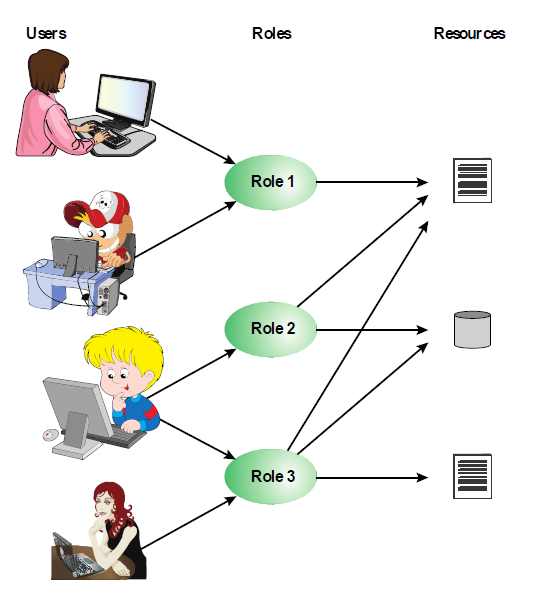
\includegraphics[scale=0.6]{../immagini/urr.png}
            \end{center}
            
        \end{figure}


        \begin{figure}[h]
            \begin{center}
                \includegraphics[scale=0.6]{../immagini/access_control_matrix.png}
            \end{center}
            \caption{Access control
            matrix
            representation of
            RBAC}
            
        \end{figure}
        \paragraph{A family of rolebased
        access
        control models}
        \begin{figure}[h]
            \begin{center}
                \includegraphics[scale=0.6]{../immagini/table.png}
            \end{center}
           
            
        \end{figure}

            \subparagraph{RBAC0}
                    \begin{figure}[h]
                        \begin{center}
                            \includegraphics[scale=0.6]{../immagini/RBAC0.png}
                        \end{center}
                    \end{figure}

                    \begin{itemize}
                        \item RBAC0 does not have role hierarchy and constraints
                        \item It contains the four types of entities:
                        \begin{itemize}
                            \item \textbf{User}: An individual (with user ID) that has access to this computer system.
                            \item \textbf{Role}: A named job function within the organization that controls this computer system (includes a description of the authority and responsibility conferred on this role).
                            \item \textbf{Permission}: An approval of a particular mode of access to one or more objects (i.e., access right, privilege, and authorization).
                            \item \textbf{Session}: A mapping between a user and an activated subset of the set of roles to which the user is assigned.
                        \end{itemize}
                    \end{itemize}
                
            \subparagraph{RBAC1}
            \begin{itemize}
                \item Role hierarchies provide a means of reflecting the hierarchical structure of roles in an organization
                \begin{itemize}
                    \item Greater responsibility implies greater authority to access resources
                    \item Inheritance of access rights from the bottom to the top
                \end{itemize}
            \end{itemize}

            \begin{figure}[h]
                \begin{center}
                    \includegraphics[scale=0.6]{../immagini/RBAC1.png}
                \end{center}
                \caption{Example of ROI
                hierarchy}
            \end{figure}

        \subparagraph{RBAC2}
        Provide a means of adapting RBAC to the specifics of
        administrative and security policies of an organization a constraint is a relationship among roles or a condition
        related to roles.

        \textbf{Types of constraints:}\\
        \begin{itemize}
            \item Mutually exclusive roles
            \begin{itemize}
                \item A user can only be assigned to one role in the set (either during a session or statically)
                \item Any permission (access right) can be granted to only one role in the set
            \end{itemize}
            \item Cardinality
            \begin{itemize}
                \item Setting a maximum number of users in a role
                \item May also limit the number of roles per user, or the number of roles a user can have per session
            \end{itemize}
            \item Prerequisite roles
            \begin{itemize}
                \item Dictates that a user can only be assigned to a particular role if it is already assigned to some other specified role
            \end{itemize}
        \end{itemize}
    
        \subsubsection{Attribute-Based Access Control}
        The authorization model can define authorizations that express conditions on properties of both the resource and the subject. The strength of this model lies in its flexibility and expressive power. However, the main obstacle to its adoption in real systems has been the concern about the performance impact of evaluating predicates on both resource and user properties for each access. 

Web services have been pioneering technologies through the introduction of the eXtensible Access Control Markup Language (XACML). There is considerable interest in applying this model to cloud services.

ABAC is distinguishable because it controls access to objects by evaluating rules against the attributes of entities, operations, and the environment relevant to a request. It relies on the evaluation of attributes of the subject, attributes of the object, and a formal relationship or access control rule defining the allowable operations for subject-object attribute combinations in a given environment. ABAC systems are capable of enforcing DAC, RBAC, and MAC concepts. Additionally, ABAC allows an unlimited number of attributes to be combined to satisfy any access control rule.
Three key elements of an ABAC system:
\begin{itemize}
    \item \textbf{Attributes} – defined for entities in a configuration;
    \item \textbf{Policy Model} – defines the ABAC policies;
    \item \textbf{Architecture Model} – applies to policies that enforce access control.
\end{itemize}
            \paragraph{Attribute}
                \subparagraph{Subject Attributes}
                A subject is an active
                entity that causes
                information to flow
                among objects or
                changes the system
                state
                and attributes define the
                identity and
                characteristics of the
                subject (id, name, job
                title, etc.)
                \subparagraph{Object attributes}
                An object (or
                resource) is a passive
                information systemrelated
                entity
                containing or
                receiving information, it have
                attributes that can be
                leverages to make
                access control
                decisions, and its attribute depend on
                the object… (owner,
                author, date, QoS,…)
                \subparagraph{environment attributes}
                The operational, technical, and situational environment or context in which information access occurs is described through contextual attributes. These attributes have largely been ignored in most access control policies. Examples of such attributes include current time, virus/hacker activity, and network security level.


                \begin{figure}[h]
                    \begin{center}
                        \includegraphics[scale=0.6]{../immagini/ABACscenario.png}
                    \end{center}
                    \caption{ABAC Scenario}
                \end{figure}
    
                \begin{figure}[h]
                    \centering
                    \begin{subfigure}
                        \centering
                        \includegraphics[scale=0.8]{../immagini/ACLRelation.png}
                    \end{subfigure}
                    \vspace{1cm}
                    \begin{subfigure}
                        \centering
                        \includegraphics[scale=0.8]{../immagini/ABACRelation.png}
                    \end{subfigure}
                    \caption{ACL and ABAC
                    relationships}
                \end{figure}

            \paragraph{Policies}

            A policy is a set of rules and relationships that govern allowable behavior within an organization, based on the privileges of subjects and how resources or objects are to be protected under specific environmental conditions. Policies are typically written from the perspective of the object that needs protection and the privileges available to subjects. Privileges represent the authorized behavior of a subject, are defined by an authority, and embodied in a policy. Other terms commonly used instead of privileges are rights, authorizations, and entitlements.

            \subparagraph{Notations}

            \begin{enumerate}
                \item S, O, and E are subjects, objects, and environments, respectively;
                \item SA\textsubscript{k} (1 $\leq$ k $\leq$ K): predefined attributes for subjects; \\
                      OA\textsubscript{m} (1 $\leq$ m $\leq$ M): predefined attributes for objects; \\
                      EA\textsubscript{n} (1 $\leq$ n $\leq$ N): predefined attributes for environments;
                \item ATTR(s), ATTR(o), and ATTR(e) are attribute assignment relations for subject s, object o, and environment e, respectively:
                    \begin{itemize}
                        \item ATTR(s) $\subseteq$ SA\textsubscript{1} $\times$ SA\textsubscript{2} $\times$ ... $\times$ SA\textsubscript{K}
                        \item ATTR(o) $\subseteq$ OA\textsubscript{1} $\times$ OA\textsubscript{2} $\times$ ... $\times$ OA\textsubscript{M}
                        \item ATTR(e) $\subseteq$ EA\textsubscript{1} $\times$ EA\textsubscript{2} $\times$ ... $\times$ EA\textsubscript{N}
                    \end{itemize}
                    Examples of attributes:
                    \begin{itemize}
                        \item Role(s) = “Service Consumer”
                        \item ServiceOwner(o) = “XYZ, Inc.”
                        \item CurrentDate(e) = “01-23-2005”
                    \end{itemize}
                \item A Policy Rule:
                    \begin{itemize}
                        \item Decides on whether a subject s can access an object o in a particular environment e;
                        \item It is a Boolean function of the attributes of s, o, and e:
                        \item Rule: can\_access(s, o, e) $\leftarrow$ f(ATTR(s), ATTR(o), ATTR(e))
                    \end{itemize}
                \item A Policy Rule Base (or policy store):
                    \begin{itemize}
                        \item May consist of a number of policy rules;
                        \item Each rule covers many subjects and objects within a security domain;
                        \item The access control decision process in essence amounts to the evaluation of applicable policy rules in the policy store.
                    \end{itemize}
            \end{enumerate}
        
        \paragraph{RBAC vs ABAC}

            
        Assume in RBAC, if there are K subject attributes and M
object attributes:

            \begin{itemize}
                \item the number of required roles are: $\prod_{k=1}^{K} range(SA_k)$
                \item the number of required permission are : $\prod_{m=1}^{M} range(SA_m)$
            \end{itemize}

            where range($\cdot$) denotes the number of possible
            values of each attribute
            In contrast ABAC is more efficient, it is just sufficient to
            add an attribute.
            \newpage
            \paragraph{Exercises}
                \subparagraph{Question} 
                Now consider the example of an online
                entertainment store that streams movies to
                users for a flat monthly fee.
                The store must enforce the following access
                control policy based on the user's age and the
                movie's content rating:

                \begin{table}[h]
                    \centering
                    \begin{tabular}{|>{\centering\arraybackslash}m{1.5cm}|>{\centering\arraybackslash}m{4cm}|>{\centering\arraybackslash}m{5cm}|}
                    \hline
                    \textbf{Movie} & \textbf{Rating} & \textbf{Users Allowed Access} \\ \hline
                    R & Age 17 and older & \\ \hline
                    PG-13 & Age 13 and older & \\ \hline
                    G & Everyone & \\ \hline
                    \end{tabular}
                    \caption{Movie Ratings and Allowed Access}
                \end{table}
                
                    \textbf{Model the access control po
                    licies
                    with RBAC and with ABAC}
                \begin{itemize}
              
                    \item RBAC To do:
                    \begin{enumerate}
                        \item Define the roles (?)
                        \item Define the permissions (?)
                        \item Define which permissions are given to each role (?)
                    \end{enumerate}

                    \item ABAC To do:
                    \begin{enumerate}
                        \item Define the roles (?)
                        \item Define attributes (?)
                        \item Define policy rules (?)
                    \end{enumerate}

                        \end{itemize}

                \subparagraph{Answer}
                        \textbf{RBAC:}

                          We can define 3 roles (R): 
                            \begin{description}
                                \item [R1]: Adult $\geq 17$ 
                                \item [R2]: Young people $\geq 13 \land < 17$
                                \item [R3]: Child $ <13$
                            \end{description}
                          And then we can define 3 permissions (P) based on rate: 
                           \begin{description}
                            \item [P1]: Can view R movie
                            \item [P2]: Can view PG-13 movie
                            \item [P3]: Can view G movie
                           \end{description}

                           \begin{table}[h]
                            \centering
                           
                            \begin{tabular}{llll}
                             & P1 & P2 & P3 \\ \cline{2-4} 
                            R1 & X & X& X\\ \cline{2-4} 
                            R2 &  & X& X\\ \cline{2-4} 
                            R3 &  &  & X\\ \cline{2-4} 
                            \end{tabular}%
                        
                            \end{table}

                        \textbf{ABAC}
                            We can define a user \textit{u} that can access of view a movie \textit{m} (the security environment \textit{e} is ignored here). We can resolve with this policy rule: \\
                            \[R1:{Can\_Access( u,m,e) \leftarrow (Age( u) \geq 17 \land Rating(m)\in \{R,PG-13,G\})} \]   
                            \[ {\lor ( Age(u) \geq 13\ \land Age(u) < 17 \land Rating( m)\in \{PG-13,G\}) \lor (Age(u) < 13 \land Rating( m)\in \{G\})}\]

                \subparagraph{Question}

                Assume now that:
                \begin{itemize}
                    \item  movies can also be classified as “New
                    Release” or “Old Release”
                    \item Users are also classified as “Premium user” or
                    “ Regular User”
                \end{itemize}

                Model RBAC and ABAC so that only Premium Users can see the New Releases.
                
                \subparagraph{Answer}

                    \textbf{RBAC:}
                        if we add two new categories, the number of rule become double, because 3 categories on the age and 2 on type of user, we have 3*2 role 
                       
                 \textbf{ABAC}
                           We can add 2 policies for resolve this:  \\
                            \[R2:{Can\_Access( u,m,e) \leftarrow (MemberType(u) = Regular \lor MemberType(u) = Premium \land MovieRelease(m) = Old )} \]
                            \[ {\lor ( MemberType(u) = Premium \land MovieRelease(m) = Old)}\]
                            \[R3: {Can\_Access( u,m,e) \leftarrow(R1 \land R2)}\]


        \subsection{Identity, credential, and access
        management (ICAM)
        and trust frameworks}

        ICAM is a comprehensive approach to managing and implementing digital identities, credentials, and access control. It was developed by the U.S. government and is designed to:
                                    \begin{itemize}
                                        \item Create trusted digital identity representations of individuals and nonperson entities (NPEs).
                                        \item Bind those identities to credentials that may serve as a proxy for the individual or NPE in access transactions.
                                        \item Use the credentials to provide authorized access to an agency’s resources.
                                    \end{itemize}

                                    A credential is an object or data structure that authoritatively binds an identity to a token possessed and controlled by a subscriber.

                                    \subsubsection {Identity Management}
                                    Identity management involves assigning attributes to a digital identity and linking it to an individual or nonperson entity (NPE), with the goal of establishing a trustworthy digital identity that is application- and context-independent. The common approach to access control is to create a digital identity for specific applications or programs, but maintaining and protecting the identity itself is often secondary to the application's mission. Unlike accounts, digital identity is not tied to job titles, duties, locations, or other attributes; these are merely attributes connected to the identity. Access control is thus based on the context and relevant user attributes rather than solely on their identity. This allows individuals to have a single digital representation that can be leveraged across departments and agencies for various purposes, including access control.

                                    \begin{figure}[h]
                                        \centering
                                        \includegraphics[scale=0.5]{../immagini/keyfunction.png}
                                        \caption{Key functions in
                                        identity
                                        management}
                                    \end{figure}

                                    The final element is lifecycle management, which includes:

                                    \begin{itemize}
                                        \item Mechanisms, policies, and procedures for protecting personal identity information.
                                        \item Controlling access to identity data.
                                        \item Techniques for sharing authoritative identity data with applications that need it.
                                        \item Revocation of an enterprise identity.
                                    \end{itemize}

                                    \subsubsection{Credential Management}
                                    A credential is an object or data structure that
                                    authoritatively binds an identity to a token possessed and
                                    controlled by a subscriber. Examples of credentials are smart cards, private/public
                                    cryptographic keys, and digital certificates. The management of the life cycle of the credential
                                    encompasses five logical components:

                                    \begin{enumerate}
                                        \item An authorized individual sponsors an individual or entity for a credential to establish the need for the credential.
                                        \item The sponsored individual enrolls for the credential.
                                        \begin{itemize}
                                            \item Process typically consists of identity proofing and the capture of biographic and biometric data.
                                            \item This step may also involve incorporating authoritative attribute data, maintained by the identity management component.
                                        \end{itemize}
                                        \item A credential is produced.
                                        \begin{itemize}
                                            \item Depending on the credential type, production may involve encryption, the use of a digital signature, the production of a smart card, or other functions.
                                        \end{itemize}
                                        \item The credential is issued to the individual or NPE.
                                        \item A credential must be maintained over its life cycle.
                                        \begin{itemize}
                                            \item Might include revocation, reissuance/replacement, reenrollment, expiration, personal identification number (PIN) reset, suspension, or reinstatement.
                                        \end{itemize}
                                    \end{enumerate}

                                    \subsubsection{Access Management}
                                    Access management and control deals with the ways entities are granted access to resources, covering both logical and physical access. This can be internal to a system or involve external elements. The purpose is to ensure proper identity verification when an individual attempts to access a security-sensitive building, computer systems, or data.

                                    \paragraph{Three support
                                    elements are
                                    needed for an
                                    enterprise-wide
                                    access control
                                    facility:}

                                    \subparagraph{Resource management}
                                    Access control is concerned with defining rules for resources that require controlled access. These rules specify credential requirements and outline the necessary user attributes, resource attributes, and environmental conditions needed to access a given resource for a particular function.

                                    \subparagraph{Privilege management}
                                    Entitlement and privilege management is concerned with establishing and maintaining the attributes that comprise an individual's access profile. These attributes represent features of an individual used to determine access decisions to both physical and logical resources. Privileges are considered attributes that can be linked to a digital identity.



                                    \subparagraph{Policy management}
                                    Governs what is allowable and unallowable in an access transaction
                            \subsubsection{Identity
                            federation} Term used to describe the technology, standards,
                            policies, and processes that allow an organization
                            to trust digital identities, identity attributes, and
                            credentials created and issued by another
                            organization. \\
                            Addresses two questions:
                                    \paragraph{Trust}   
                                    How do you trust identities of individuals from external
                                    organizations who need access to your systems?
                                    \\
                                    Trust, identity, and attributes have become primary concerns in internet business, network service providers, and similar fields. Consider the case of e-commerce: the attributes you need to know about someone to deal with them depend on the specific situation. These attributes might include professional registration or license number, organization and department, staff ID, security clearance, customer reference number, credit card number, unique health identifier, allergies, blood type, Social Security number, address, citizenship status, social networking handle, pseudonym, and more. The attributes that must be known and verified to permit a transaction are context-dependent. This issue extends beyond just e-commerce.

                                    \paragraph{Identity Information exchange approaches} How do you vouch for identities of individuals in your
                                    organization when they need to collaborate with external
                                    organizations? \\ 
                                        \begin{figure}[h]
                                            \centering
                                            \includegraphics[scale=0.5]{../immagini/identity_information_exchange.png}
                                           
                                        \end{figure}
    
                                    
                                    \begin{description}
                                        \item[Relying party:] 
                                        \begin{itemize}
                                            \item requires that the user has been authenticated to some degree of assurance,
                                            \item attributes provided by the identity service provider are accurate,
                                            \item identity service provider is authoritative for those attributes.
                                        \end{itemize}
                                        
                                        \item[Identity service provider:] 
                                        \begin{itemize}
                                            \item requires assurance of accurate user information,
                                            \item if sharing information, the relying party will use it according to contractual terms and the law.
                                        \end{itemize}
                                        
                                        \item[User:] 
                                        \begin{itemize}
                                            \item requires assurance that the identity service provider and relying party can be trusted with sensitive information,
                                            \item that they will respect user preferences and privacy.
                                        \end{itemize}
                                        
                                        \item[All parties:] 
                                        \begin{itemize}
                                            \item want to ensure that the practices described by other parties are actually implemented and reliable.
                                        \end{itemize}
                                    \end{description}

                                    \subparagraph{Open Identity Trust framework}
                                    A trust framework functions as a certification program, enabling a party who accepts a digital identity credential (the relying party) to trust the identity, security, and privacy policies of the party who issues the credential (the identity service provider) and vice versa. Developed by a community with similar goals and perspectives, a trust framework defines the rights and responsibilities of the community's participants, specifies policies and standards, and outlines the processes and procedures that provide assurance. Different trust frameworks can exist, allowing participants to tailor them to meet their specific needs.

                                    \begin{description}
                                        \item[OpenID:] 
                                        An open standard that allows users to be authenticated by certain cooperating sites using a third party service.
                                        
                                        \item[OIDF:] 
                                        OpenID Foundation is an international nonprofit organization of individuals and companies committed to enabling, promoting, and protecting OpenID technologies.
                                        
                                        \item[ICF:] 
                                        Information Card Foundation is a nonprofit community of companies and individuals working together to evolve the Information Card ecosystem.
                                        
                                        \item[OITF:] 
                                        Open Identity Trust Framework is a standardized, open specification of a trust framework for identity and attribute exchange, developed jointly by OIDF and ICF.
                                        
                                        \item[OIX:] 
                                        Open Identity Exchange Corporation is an independent, neutral, international provider of certification trust frameworks conforming to the OITF model.
                                        
                                        \item[AXN:] 
                                        Attribute Exchange Network is an online Internet-scale gateway for identity service providers and relying parties to efficiently access user asserted, permissioned, and verified online identity attributes in high volumes at affordable costs.
                                    \end{description}
                                    

                                    \begin{figure}[h]
                                        \centering
                                        \includegraphics[scale=0.5]{../immagini/identity_information_exchange2.png}
                                       
                                    \end{figure}
                                    \newpage
\section{Database and
Data Center Security
Computer}
                Reasons database
                security has not
                kept pace with the
                increased reliance
                on databases are:   \\                 
                \begin{itemize}
                    \item There is a dramatic imbalance between the complexity of modern database management systems (DBMS) and the security techniques used to protect them.
                    \item Databases have sophisticated interactions. The Structured Query Language (SQL) protocol is complex.
                    \item There is an increasing reliance on cloud technology to host part or all of the corporate database.
                    \item Effective database security requires a strategy based on a full understanding of the security vulnerabilities of SQL.
                    \item The typical organization lacks full-time database security personnel.
                    \item Most enterprise environments consist of a heterogeneous mixture of database platforms, enterprise platforms, and OS platforms, creating an additional complexity hurdle for security personnel.
                \end{itemize}
            
            \subsection{DBMS}
                	\paragraph{Databases}
                    A database is a structured collection of data stored for use by one or more applications. It contains the relationships between data items and groups of data items, and it can sometimes include sensitive data that requires security measures. A query language provides a uniform interface to the database for both users and applications.
                    
                    \paragraph{DMBS}
                        A database management system (DBMS) is a suite of programs designed for constructing and maintaining databases. It offers ad hoc query facilities to multiple users and applications, allowing flexible and efficient access to the stored data.
                    
                        
                        \begin{figure}[h]
                            \centering
                            \includegraphics[scale=0.5]{../immagini/Dbmsarchiteture.png}
                            \caption{DBMS architecture}
                        \end{figure}

                        \subparagraph{Security Requirements}
                        Database systems generate security requirements that exceed the capabilities of typical OS-based security mechanisms or stand-alone security packages. While operating system security mechanisms generally control read and write access to entire files, they are inadequate for limiting access to specific records or fields within those files. DBMSs, however, require such detailed (granular) access control and typically enable access controls over a broader range of commands, such as selecting, inserting, updating, or deleting specified items in the database. This necessitates specifically designed security services and mechanisms integrated with the DBMS.

                    \paragraph{Relational Database}
                    A table in a database consists of rows and columns, where each column holds a particular type of data and each row contains specific values for each column. Ideally, one column contains unique values, serving as an identifier or key for that row. This structure allows for the creation of multiple tables linked by a unique identifier present in all tables. A relational query language is used to access the database, enabling users to request data that meet specific criteria. This query language is declarative, meaning it specifies what data to retrieve rather than how to retrieve it.
                        \subparagraph{Elements:}
                        \begin{itemize}
                            \item \textbf{Relation}: A flat table in a file.
                            \item \textbf{Tuple}: Rows (records) of the table.
                            \item \textbf{Attribute}: Columns (fields) of the table.
                            \item \textbf{Primary key}: Uniquely identifies a row; consists of one or more column names.
                            \item \textbf{Foreign key}: Links one table to attributes in another; it’s a primary key in another table.
                            \item \textbf{View/virtual table}: The result of a query that returns selected rows and columns from one or more tables. Views are often used for security purposes to provide restricted access to certain rows or columns.
                        \end{itemize}

                        \begin{figure}[h]
                            \centering
                            \includegraphics[scale=0.5]{../immagini/basic_terminology.png}
                            \caption{Basic Terminolgy}
                        \end{figure}
                    
                    \paragraph{SQL}
                    SQL is a standardized language used to define schemas, manipulate data, and query information in a relational database. While there are several similar versions of the ANSI/ISO standard, all adhere to the same basic syntax and semantics. SQL statements can be employed to create tables, insert and delete data within those tables, create views, and retrieve data through query statements.
            
                    \paragraph{Question \& Examples}
                        \subparagraph{Question}
                        \begin{figure}[h]
                            \centering
                            \includegraphics[scale=0.5]{../immagini/question.png}
                            
                        \end{figure}    

                        \subparagraph{Answer}
                            Only rows with Member-ID equals to 91, 36 can be added to the table
            \subsection{SQL injection attacks}
            SQL injection is one of the most prevalent and dangerous network-based security threats, where malicious SQL commands are sent to a database server. The most common goal of such attacks is the bulk extraction of data. However, depending on the environment, SQL injection can also be exploited to modify or delete data, execute arbitrary operating system commands, and launch denial-of-service (DoS) attacks.

                    \subsubsection{SQL Injection Attacks}
                    An SQL injection (SQLi) attack is designed to exploit the dynamic nature of modern web application pages, which are no longer static and often query databases on servers to access sensitive data. By sending malicious SQL commands to the database server, an SQLi attack can extract large amounts of data, modify or delete data, execute arbitrary operating system commands, and even launch denial-of-service (DoS) attacks.

                    \begin{figure}[h]
                        \centering
                        \includegraphics[scale=0.5]{../immagini/Injection_attack.png}
                        \caption{A typical SQL
                        injection
                        attack}
                    \end{figure}    

                    \paragraph{Injection Technique}
                    The SQLi attack typically works by prematurely terminating a text string and appending a new command, because the inserted command may have additional strings
                    appended to it before it is executed the attacker terminates the injected string with a comment mark "- -", subsequent text is ignored at execution time

                    \paragraph{Example of SQLi}
                    As a simple example, consider a script that builds an SQL query
                    by combining predefined strings with text entered by a user:
                    \begin{lstlisting}[language=SQL]
                        var ShipCity;
                        ShipCity = Request.form ("ShipCity");
                        var sql ="SELECT * FROM OrdersTable WHERE ShipCity = '" + ShipCity +" ' ";
                    \end{lstlisting}
                    The intention of the script's designer is that a user will enter the
                    name of a city. For example, if the user enters Pisa, then the
                    following SQL query is generated:

                    \begin{lstlisting}[language=SQL]
                        SELECT * FROM OrdersTable WHERE ShipCity = 'Pi  sa';
                    \end{lstlisting}
                
                
                



















































                \end{document}

    